\documentclass[10pt,reqno, usenames]{article}
\usepackage[a4paper, hmargin={2.8cm, 2.8cm}, vmargin={2.5cm, 2.5cm}]{geometry}

% Language setting
% Replace `english' with e.g. `spanish' to change the document language
\usepackage[danish]{babel}
\usepackage{hyperref}
\usepackage[utf8]{inputenc}
\usepackage{array}
\usepackage{xcolor}
\usepackage{amsmath}
\usepackage{amssymb}
\usepackage{pgfplots}
\interfootnotelinepenalty=10000
\usepackage{tikz}
\usepackage{booktabs}
\usepackage{amsmath}
\usepackage{fancyhdr,setspace} 
\usepackage[breakable]{tcolorbox}
\pagestyle{fancy}
\lhead{Noter til Erhvervsøkonomi, Levi van Boekel}
\rhead{2. semester, Økonomi}
\onehalfspacing


% Useful packages
\usepackage{amsmath}
\usepackage{graphicx}
\setlength{\parindent}{0pt}
\usepackage[colorlinks=true, allcolors=blue]{hyperref}
\title{Noter til Erhvervsøkonomi}
\author{Levi van Boekel}

\begin{document}
\maketitle


\tableofcontents

\newpage
\vspace*{\fill}
\begin{center}
    \textbf{Denne side er med vilje efterladt uden indhold.}
\end{center}
\vspace*{\fill}

\newpage
\section{Regnskab}

\subsection{Principper og antagelser}
\subsubsection{Regnskabets 4 grundlæggende antagelser}
Der ligger 4 overordnede antagelser til grund for årsregnskabets og dets komponenter. Disse er givet ved: 

\begin{enumerate}
    \item \textbf{Økonomisk enhed ('economic entitiy')}
    \item \textbf{Regnskabsperiode}
    \item \textbf{Going concern}
    \item \textbf{Ingen inflation ('stable dollar')}
\end{enumerate}

Den første antagelse (1) beskriver, at der altid skal være en klar afgrænsning af den økonomiske enhed, der aflægger regnskab (f.eks. et enkelt selskab). Det er her vigtigt at skelne mellem et konsolideret regnskab, der dækker hele koncernen, dvs. moderselskabet ('parent') og alle dens direkte og indirekte ejede datterselskabet ('subsidaries'), og et ikke konsolideret regnskab, der kun omfatter et enkelt selskab. 

\hspace{10 pt}

Den anden antagelse (2) beskriver, at perioden for hvilken der aflægges regnskab skal være klart afgrænset (f.eks. kalenderåret eller andre et-årige konstellationer). 

\hspace{10 pt}

Den tredje antagelse (3) er et udtryk for, at virksomheden fortsat vil være aktiv i tiden efter regnskabsperioden. Derfor vil værdierne af aktiverne vurderes ud fra den forudsætning, at de fortsat skal anvendes i virksomheden og ikke, hvad de kan indbringe ved øjeblikkeligt salg. I tilfælde af, at en virksomhed er truet af konkurs, vil antagelsen være misvisende. 

\hspace{10 pt}

Den fjerde antagelse (4) beskriver, at regnskabets elementer måles i årets løbende valuta og der således ikke tages højde for inflation. I perioder med høj inflation kan antagelsen være misvisende og føre til, at værdien af aktiverne (og dermed egenkapitalen) undervurderes. 

\subsubsection{Grundlag for værdiansættelse}
Der er 4 måder at værdiansætte på, disse er: 

\begin{enumerate}
    \item \textbf{Markedsværdi} ('fair market value'), der beskriver, hvad aktivet kunne sælges for på markedet
    \item \textbf{Genanskaffelsesomkostningen} ('replacement cost'), der beskriver, hvad det ville koste at købe et tilsvarende aktiv på markedet i dag
    \item \textbf{Indkøbspris} ('original cost'), der beskriver, hvad aktivet kostede den gang det blev anskaffet
    \item \textbf{Nutidsværdi} ('present value'), der beskriver den tilbagediskonteret værdi af fremtidig cashflow generet af aktivet (mere om nutidsværdi i investeringsafsnittet)
\end{enumerate}

Det gælder, at: 


\begin{itemize}
    \item Kontanter, kortfristet gæld, kundetilgodehavender og værdipapirer opgøres oftest i markedsværdi. 
    \item Lagervarer opgøres til anskaffelsesprisen eller genanskaffelsesprisen, hvis den er lavere. 
    \item Jord, bygninger, maskiner og langsigtede aktieinvesteringer opgøres til anskaffelsesprisen, dog fratrukket afskrivningerne.
    \item Langfristet gæld og langfristede tilgodehavender opgøres ved nutidsværdien. 
\end{itemize}

\subsubsection{Regnskabets 4 grundlæggende principper}
De fire grundlæggende principper i årsregnskabet er: 

\begin{enumerate}
    \item \textbf{Objektivitet}
    \item \textbf{Matching}
    \item \textbf{Indregning af indkomst}
    \item \textbf{Konsistens}
\end{enumerate}

Det første princip (1) beskriver, at den information, der ligger til grund for regnskabet skal være dokumenterbar og pålidelig. 

\hspace{10 pt}

Det andet princip (2) er et udtryk for, at omkostninger skal bogføres i samme regnskabsperiode som de indtægter, der følger af disse omkostninger. I praksis implementeres matching principper ved, at (1) udgifterne til en investering bogføres som et aktiv, når de afholdes og (2) aktivet afskrives over den periode, hvor indtægterne realiseres. Altså: matchingprincippet bidrager til, at regnskabet giver et retvisende billede af virksomhedens finansielle situation i en given periode. 

\hspace{10 pt}

Det tredje princip (3) besvarer spørgsmålet om, hvornår en indkomst må bogføres i regnskabet. Her gælder det grundlæggende, at følgende kriterer skal være opfyldt: (1) størstedelen af produktions- og salgsarbejde er færdiggjort, (2) indkomstens størrelse er kendt, (3) størstedelen af omkostningerne er afholdt og resten kendes og (4) betaling er sikret med stor sandsynlighed. I praksis fortolkes det sådan, at virksomheder må bogføre indkomsten, når en vare er leveret. 

\hspace{10 pt}

Det fjerde princip beskriver, at virksomheder, som udgangspunkt, skal benytte samme grundlag i hver regnskabsperiode. Hermed sikres det, at regnskaberne bliver sammenlignelige over tid. Der kan således kun i særlige tilfælde ske skift i regnskabspraksis (og i givet fald skal det fremgå klart). 

\subsection{Bogholderi og t-konti}
Det dobbelte bogholderi er grundlæggende centreret omkring regnskabsligning, der tilsiger, at: 

\begin{equation}
     \text {Aktiver} = \text {Passiver} + \text {Egenkapital} 
\end{equation}

Heraf følger, at balancen altid skal balancere. Derfor er bogholderiet bygger op omkring en kredit- og en debitkonto, der sikrer, at en transaktion på kreditkontoen modsvares af en tilsvarende modtransaktion på debitkontoen. I praksis gælder det da, at \textbf{aktivkontoen har en debetsaldo}, hvor det gælder, at:
\begin{itemize}
    \item Saldoen øges ved at debitere kontoen 
    \item Saldoen mindskes ved at kreditere kontoen
\end{itemize}
Det modsatte gælder ved en \textbf{passivkonto, der har en kreditsaldo}. Her gælder, at:  
\begin{itemize}
    \item Saldoen øges ved at kreditere kontoen 
    \item Saldoen mindskes ved at debitere kontoen
\end{itemize}
Intuitionen bag ovenstående er, at en stigning i aktiverne øger virksomhedens værdier og dermed debiteres, mens en stigning i passiverne øger kravene mod virksomhedens aktiver fra f.eks. långivere eller ejere, og dermed krediteres. \textbf{På en t-konto vil debit altid være på venstre side, mens kredit vil være på højre side}. Et eksempel på bogføringen af en given transaktion er givet ved nedenstående, hvor en virksomhed har solgt varer for 5000 kr. på kredit. 

\begin{figure}[h]
     \centering
     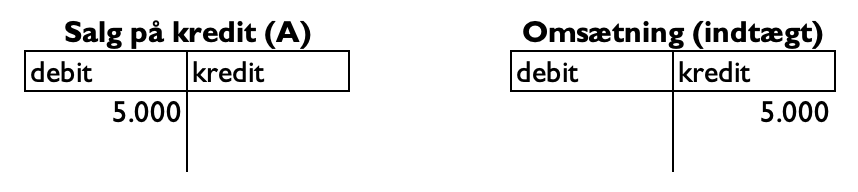
\includegraphics[scale=0.75]{t-konti 1.png}
     \caption{Bogføring af salg på kredit}
     \label{Figur 1}
\end{figure} 

Her er intuitionen netop, at salget på kredit øger virksomhedens aktiver (debit på aktiv-siden), men samtidig også øger kreditorernes forpligtelser overfor virksomheden, hvorfor omsætningen krediteres. 

\begin{tcolorbox}[colback=red!5!white, colframe=red!50!black, title=Eksempel på bogføring af en række transaktioner]
Antag at virksomheden 'Viking Væv \& Design' har følgende transaktioner i løbet af året (2014): 

\begin{enumerate}
   \item Indbetaler 492.000 kr. i egenkapital
\item Låner 500.000 kr. i banken til en årlig rente på 10 pct.
\item Køber produktionsanlæg for i alt 400.000 kr. (kontant)
\item Køber diverse råvarer og hjælpematerialer til i alt 300.000 kr. (kontant)
\item  Producerer efter bestilling 28 møbler til en samlet omsætning på 1.400.000 kr.
\item Betaler diverse udgifter og honorar for 2014, 70.000 kr.
\item Modtager delvis betaling for leverede møbler, 600.000 kr.
\item Betaler husleje for hele 2014 samt for 1. kvartal 2015, 325.000 kr.
\item Opgør råvarelageret ultimo 2014 til en samlet værdi af 100.000 kr.
\item Betaler renter og afdrag på banklånet, 120.000 kr.
\item Afskriver 25pct. af den bogførte værdi på produktionsanlægget
\end{enumerate}

Posteringerne er enkeltvis bogført i vedlagte appendix, se \ref{Figur 2}. De aggregerede konti er anført nedenfor: 

\centering  
\vspace{10pt}
    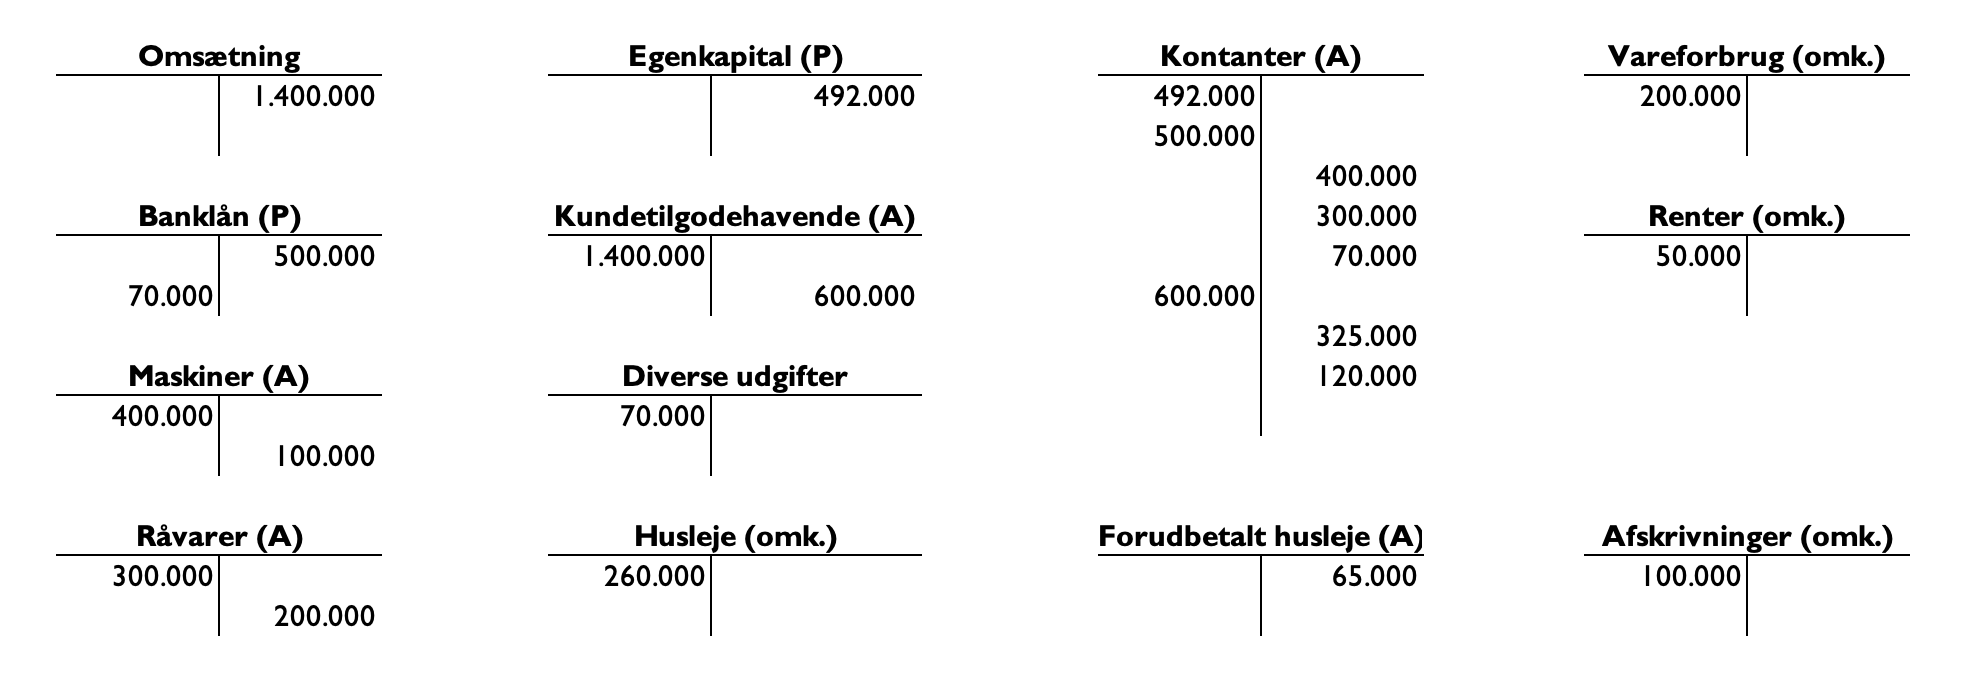
\includegraphics[width=0.75\linewidth]{aggregerede konti.png}
\vspace{10pt}

På baggrund af de aggregerede t-konti er nedenstående balance- og resultatopgørelse konstrueret: 

\centering  
\vspace{10pt}
    \includegraphics[width=0.75\linewidth]{resultatopgørelse og balance.png}
\vspace{10pt}

\end{tcolorbox}

\subsubsection{Note om momsafstemning}
Generelt gælder det, at \textbf{salgsmoms krediteres}, fordi der her er tale om moms som virksomheden har opkrævet fra kunderne og skal betale til skattemyndighederne. Omvendt, \textbf{debiteres købsmoms}, da virksomheden kan kræve denne moms tilbage fra skattemyndighederne og det dermed udgør et aktiv for virksomheden. Efter et regnskabsår vil kontiene da være givet ved nedenstående, hvor værdierne i hhv. købs- og salgsmoms er arbitrære. \\
\begin{figure}[t]
     \centering
     \includegraphics[scale=0.3]{Moms, før afstemning.png}
     \caption{Momskonti før afstemning}
     \label{Figur 1}
\end{figure} 
Når selve afstemningen finder sted bliver kontoerne for købs- og salgsmoms nulstillet ved at kreditere købsmomskontoen og debitere salgsmomskontoen med deres indestående. Samtidig oprettes en ny konto ved navn momsafregning, hvor købsmomsen krediteres og salgsmomsen debiteres. Dette er gjort nedenfor: 

\begin{figure}[h]
     \centering
     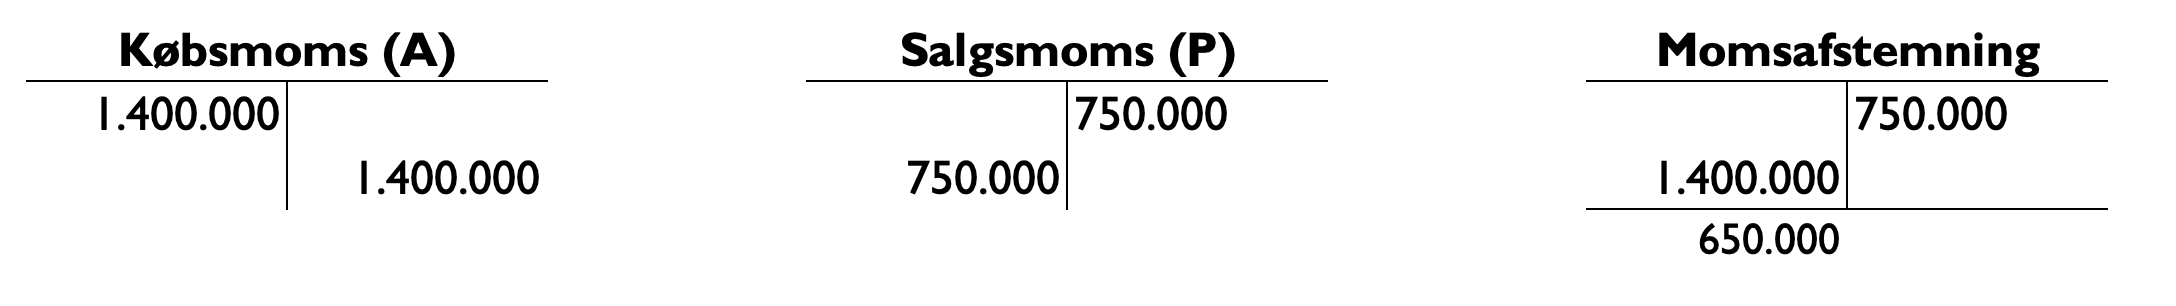
\includegraphics[scale=0.3]{Momsafstemning.png}
     \caption{Momskonti efter afstemning}
     \label{Figur 1}
\end{figure} 

Det er her værd at bemærke, at det endelige beløb ($650.000$) indgår i balancen som \textbf{aktiv og dermed skal debiteres, hvis købsmoms $>$ salgsmoms}, mens det indgår som \textbf{passiv og dermed skal krediteres, hvis købsmoms $<$ salgsmoms}. Det gælder, da virksomheden i det første tilfælde vil have penge til gode hos skattemyndighederne, hvorfor aktiverne stiger som følge af afstemningen, mens virksomheden i det andet tilfælde vil skylde penge til myndighederne, hvorfor selskabets forpligtelser stiger og beløbet dermed skal krediteres. 

\subsubsection{Bogføring af komplekse transaktioner}
Der vil sommetider opstå transaktioner, der kræver en vis grad af kreativitet af bogføre korrekt. I afsnittet gennemgås bogføringen af flg. posteringer, der ikke falder indenfor nogle skabeloner: 
\begin{enumerate}
    \item Kursgevinst/tab (kontanter)
    \item Efterposteringer i fald af, at private omkostninger er bogført som virksomhedsudgifter
    \item Opkøb af anden virksomhed
    \item Fund af varer, der er blevet afskrevet i en tidligere periode
    \item Kursgevinst/tab (værdipapirer)
\end{enumerate}

Ved \textbf{kursgevinst/tab (1)} påvirkes omsætningen (ved gevinst) og omkostninger (ved tab), samt kontantkontoen. Antag, at en virksomhed har opnået en kursgevinst/tab på 20.000 kinesiske Yuan. Her vil kontiene se således ud, hvor de øverste konto er de berørte konti ved et kurstab og de nederste er de berørte konti ved kursgevinst. 

\begin{figure}[h]
     \centering
     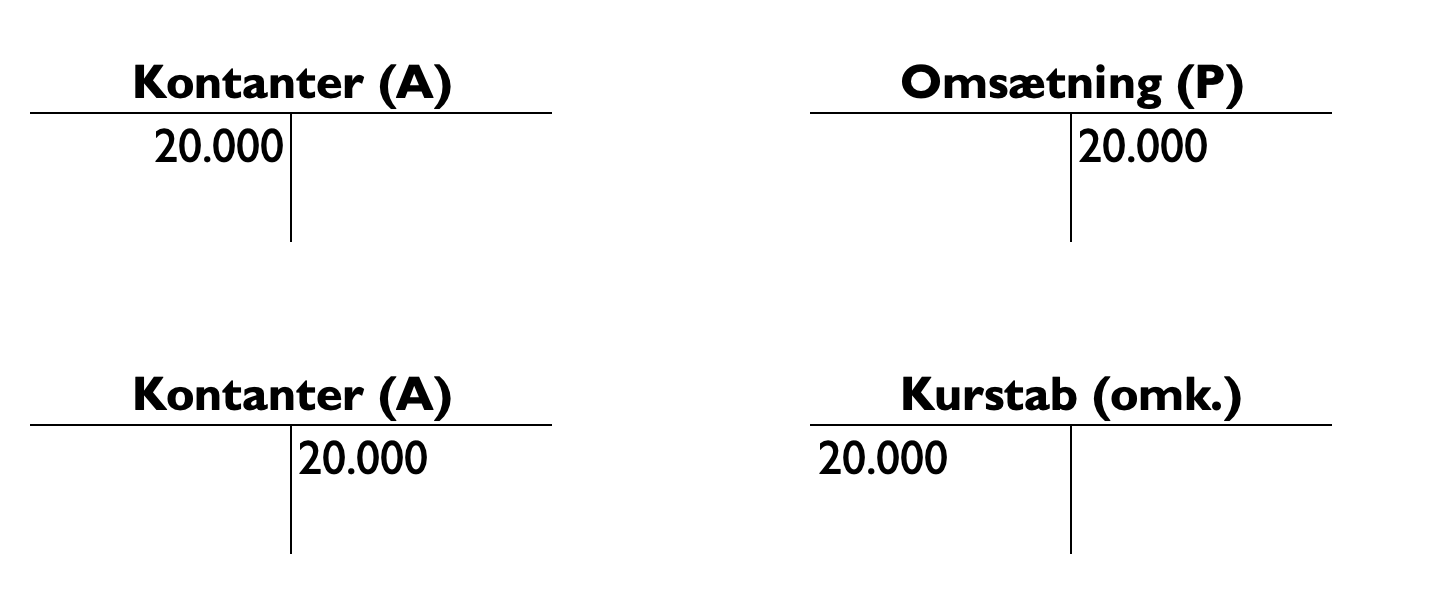
\includegraphics[scale=0.25]{kurs.png}
     \caption{Bogføring af kursgevinst/tab}
     \label{Figur 1}
\end{figure} 

I fald af en efterpostering, der skal tage højde for, at \textbf{private omkostninger er bogført som virksomhedsudgifter}, vil flere konti berøres og det vil i mange tilfælde afhænge af, hvilke omkostninger, der er tale om. Uanset tilfælde, vil det nedenstående flow dog gælde. Her er det antaget, at virksomheden - uretmæssigt - har bogført et klubbesøg på 4000 kr. som udgift og beløbet i stedet skal betales som et ekstraordinært udbytte til ejeren. 

\begin{figure}[h]
     \centering
     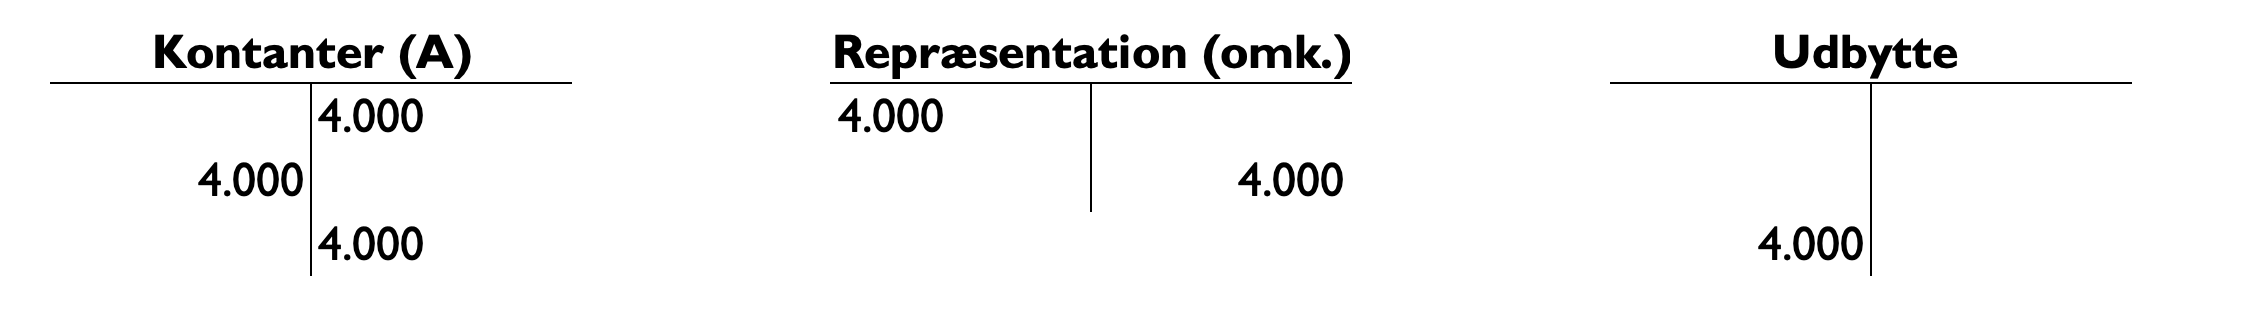
\includegraphics[scale=0.3]{private udgifter.png}
     \caption{Efterpostering ved privat udgifter afholdt af virksomheden (som udbytte)}
     \label{Figur 1}
\end{figure} 

I første række krediteres kontantbeholdningen med 4000, samtidig med, at repræsentation debiteres med samme beløb, idet virksomheden har afholdt udgiften. Herefter nulstilles kontiene ved at debitere kontantbeholdningen og kreditere repræsentationskontien. Afsluttende krediteres kontantkontoen med 4000 (for at vise, at det ekstraordinære udbytte er betalt), mens udbyttekontoen debiteres med samme beløb. Hvis ejeren ikke modtager et ekstraordinært udbytte, men i stedet skal betale pengene tilbage til virksomheden. Vil det se således ud: 

\begin{figure}[h]
     \centering
     \includegraphics[scale=0.3]{udlæg til ejer.png}
     \caption{Efterpostering ved privat udgifter afholdt af virksomheden (som udlæg)}
     \label{Figur 1}
\end{figure} 

Forskellen er her, at debiteringen af kontanterne modsvares af en debiteringen af kontoen 'udlæg til ejer', der krediteres, når ejer indbetaler midlerne. Ved indbetalingen vil kontantbeholdningen debiteres. 

\vspace{10 pt}

\textbf{Bogføring af opkøb af en virksomhed (3)} er forskellig alt afhængigt af, hvor stor virksomhedens aktiver og passiver er, men grundlæggende kan alle køb bogføres efter nedenstående logik. Antag, at den Randers baserede virksomhed 'Nordic Vape' opkøbes af amerikanske 'Juul' for 550.000 kr., idet Juul vil gøre deres indtog på det danske marked. 'Nordic Vape' har på tidspunktet af salget følgende aktiver og passiver: færdigvarer (1.000.000 kr.), råvarer (520.000 kr.), langfristet gæld (1.350.000 kr.) og egenkapital (170.000 kr.). Den grundlæggende erkendelse er her, at Nordic Vapes egenkaptial \textbf{ikke} indgår i Juuls' balance. Deres t-konti vil da påvirkes således: 

\begin{figure}[h]
     \centering
     \includegraphics[scale=0.3]{opkøb.png}
     \caption{Bogføring af opkøb}
     \label{Figur 1}
\end{figure} 

Altså: kontantkontoen krediteres med 550.000, mens råvarer og færdigvare kontoen debiteres med hhv. 520.000 og 1.000.000. Samtidig krediteres langfristet gæld med 1.350.000. Afsluttende debiteres goodwill kontoen med 380.000, der netop er forskellen mellem egenkapitalen i Nordic Vape og salgsprisen. Intuitionen bag, at egenkapitalen ikke indgår er, at en køberen erhverver virksomhedens nettoaktiver og ikke egenkapitalen. Man kan dermed tale om, at egenkapitalen i den erhvervede virksomhed 'opløses' og det, der faktisk erhverves, dermed er aktiverne og forpligtelserne. Egenkapitalen fra den erhvervede virksomhed bliver ikke konsolideret, da det ville indebære en dobbelttælling af værdi – egenkapitalen repræsenterer jo allerede værdien af de aktiver minus forpligtelser, som nu er købers.


\vspace{10 pt}

\textbf{I tilfælde af, at der findes værdier, der er blevet afskrevet i en tidligere periode (4)}, er den regnskabsmæssige konsekvens forholdsvis simpel og illustreret nedenfor, hvor der findes råvarer for 5000 kr. 

\begin{figure}[h]
     \centering
     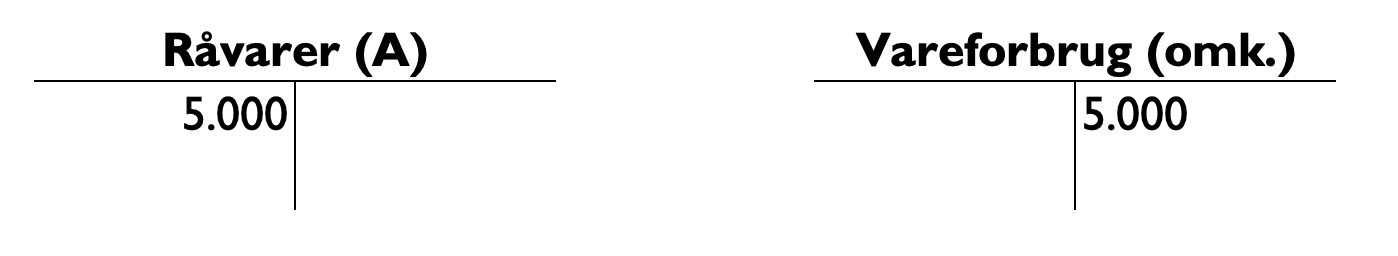
\includegraphics[scale=0.3]{afskrivning.png}
     \caption{Bogføring af fund af råvarer}
     \label{Figur 1}
\end{figure} 

\vspace{10 pt}

\textbf{Ved kursgevinst/tab på aktier (5)} minder bogføringen i høj grad om den, der er beskrevet under punktet for kursgevinst/tab ved valuta. Antag f.eks. at en virksomhed i primo 2022 købte Novo aktier for 510.000 kr. og disse i slut 2022 havde en værdi på 650.000. Kursgevinst ville da fremgår som følger: 

\begin{figure}[h]
     \centering
     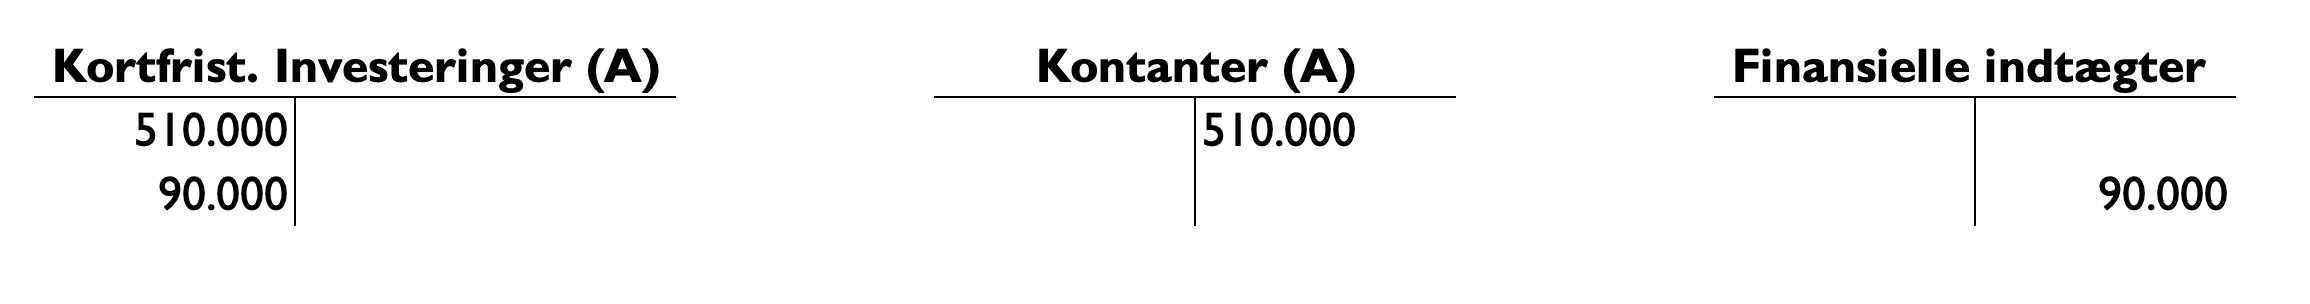
\includegraphics[scale=0.3]{kursgevinst, aktier.png}
     \caption{Bogføring af kursgevinst på aktier}
     \label{Figur 1}
\end{figure} 

Ved et tilsvarende tab, ville de kortfristede investeringer skulle krediteres, mens finansielle udgifter ville skulle debiteres. 

\subsection{Direkte og indirekte pengestrømsopgørelse}
Når pengestrømmen opgøres \textbf{direkte}, vil man regnskabsmæssigt skulle holde styr på samtlige bruttobevægelser i løbet af et givent år. Det kunne se ud som nedenfor: 

\begin{figure}[h]
     \centering
     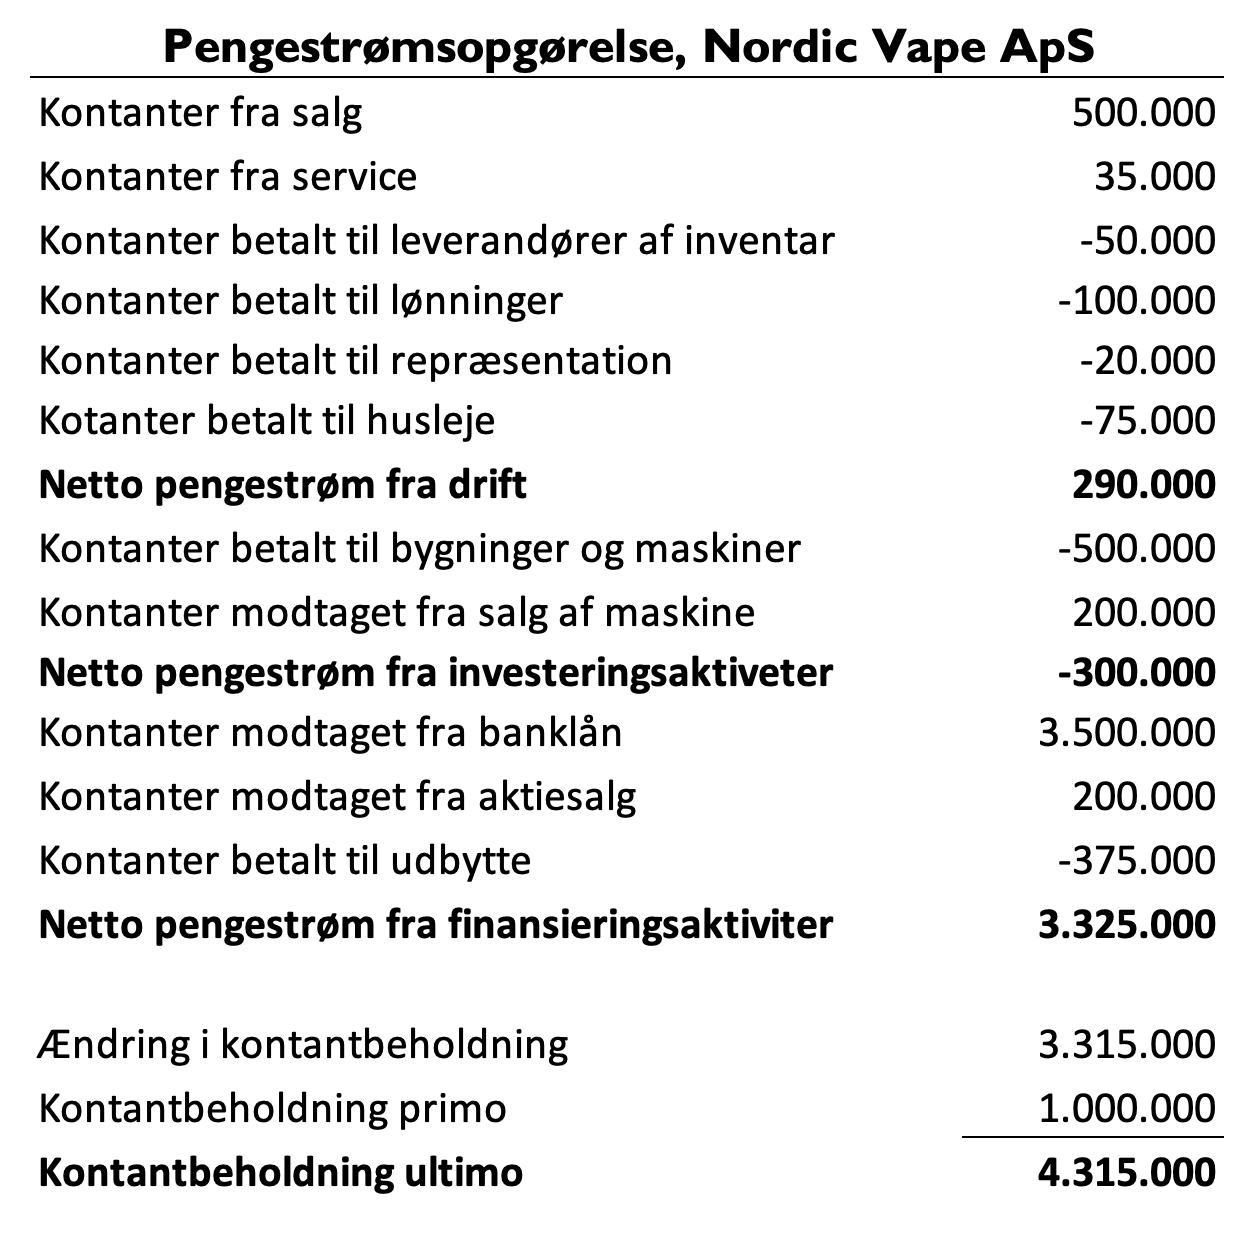
\includegraphics[scale=0.3]{Pengestrømsopgørelse, direkte.png}
     \caption{Pengestrømsopgørelse, direkte}
     \label{Figur 1}
\end{figure}

Bemærk, at hver komponent i opgørelsen er summen af de aggregerede transaktioner indenfor de respektive områder. En ung startup vil typisk have et stort positivt cashflow fra finansieringsaktiviteter (optager gæld, sælger aktier, m.m.) og et lille (måske endda negativt) cash flow fra driften. Omvendt vil det være for mere veletablerede virksomheder, der i højere grad har et positivt cash flow fra driften og ofte negativ pengestrøm fra finanseringsaktiviteter (betaler udbytte, lån tilbage m.m.). I praksis (og særligt for store virksomheder), er det et stort arbejde forbundet med at udarbejde den direkte pengestrømsopgørelse, hvorfor der i de fleste virksomheder udarbejdes en indirekte pengestrømsopgørelse. 

\vspace{10 pt}

\textbf{Den indirekte pengestrømsopgørelse} tager udgangspunkt i balancen og resultatopgørelsen og prøver på baggrund af de foreliggende tal at estimere pengestrømmen i perioden. Den grundlæggende tanke er her, at ændringer på balancen sammenlagt med information fra balancen nødvendigvis må være et udtryk for pengestrømmenene. Betragt f.eks. nedenstående balance for virksomheden 'M-karrusel':

\begin{figure}[h]
     \centering
     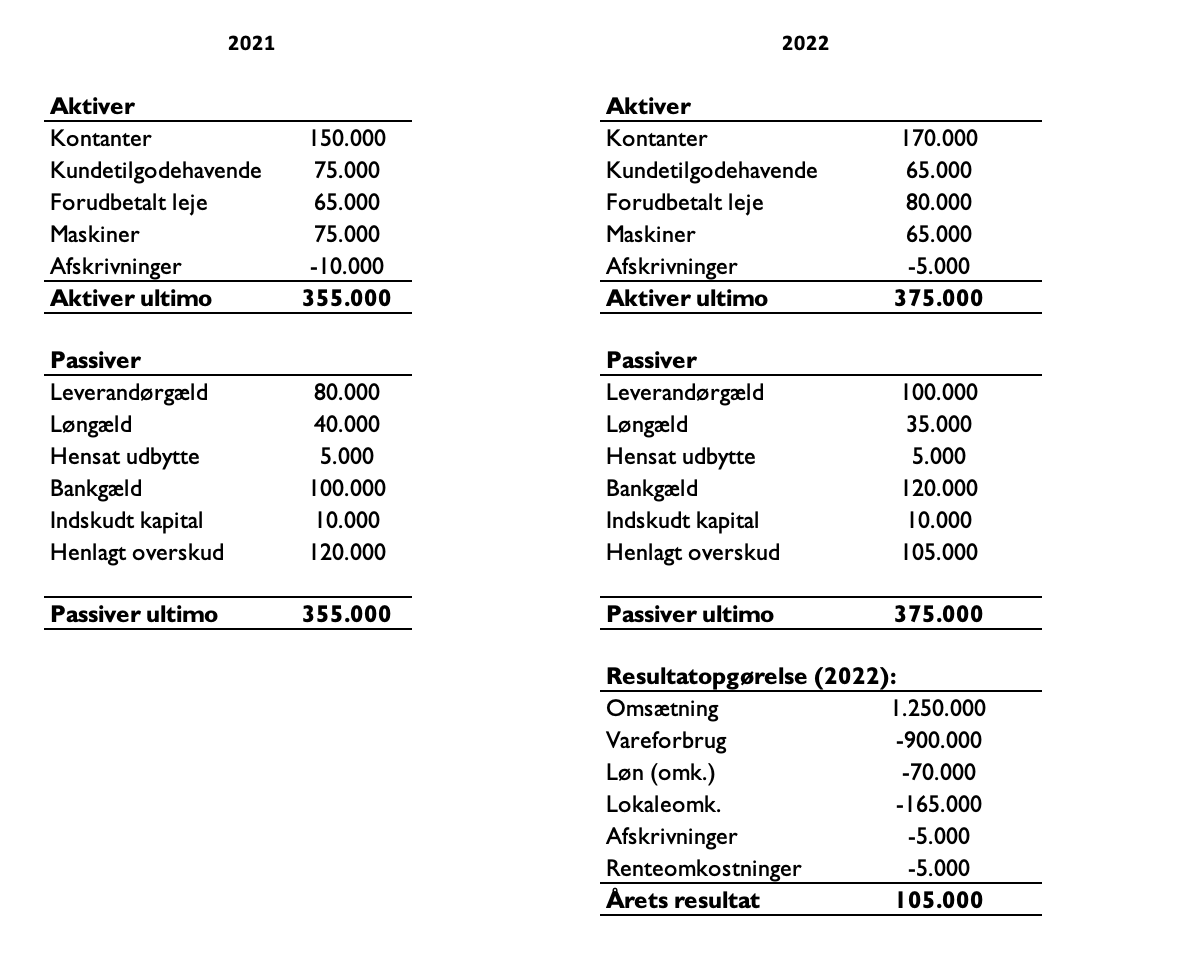
\includegraphics[scale=0.5]{Balance, M karusel.png}
     \caption{Balance, M-karrusel}
     \label{Figur 1}
\end{figure}

Af resultatopgørelsen fremgår det, at virksomheden havde en omsætning på 1.250.000 kr., samtidig med, at kundetilgodehavende faldt fra 75.000 til 60.000. Heraf må det nødvendigvis følge, at pengestrømmen fra salg er 1.260.000 kr. ($1.250.000 - (65.000 - 75.000)$. På tilsvarende vis kan pengestrømmen til leverandører (dvs. hvor mange penge, der blev betalt til leverandører), ved først at betragte vareforbruget, og herefter leverandørgælden. Dette gælder, da vareforbruget fortæller, at der blev videresolgt varer til en given pris, og leverandørgælden viser hvor mange af de midler der blev betalt kontant eller på kredit. I ovenstående tilfælde er pengestrømmen til leverandører givet ved 880.000 kr. ($900.000 - (100.000 - 80.000)$). Den samlede pengestrøm til lønninger i det givne regnskabsår kan ligeledes aflæses, idet resultatopgørelsen fortæller, at de samlede lønomkostninger i perioden var 70.000 samtidig med, at løngælden faldt fra 40.000 til 35.000, altså er pengestrømmen til lønninger givet ved 75.000 kr. ($70.000 - (35.000 - 40.000)$). Pengestrømmen fra driften som helhed kan opgøres ved hjælp af nedenstående metode, der starter med at betragte årets resultat, hertil justerer for ikke kontante poster og afslutningsvis tager højde for ændringer i arbejdskapital \footnote{Arbejdskapitalen består af aktiver, der omsættes til kontanter inden for et regnskabsår (f.eks. kundetilgodehavender, varelager) og kortfristede forpligtelser, der skal betales inden for samme periode (f.eks. leverandørgæld, kortfristet gæld). Kontanter indgår ikke, da de allerede er en likvid form for aktiv.)}

\begin{figure}[h]
     \centering
     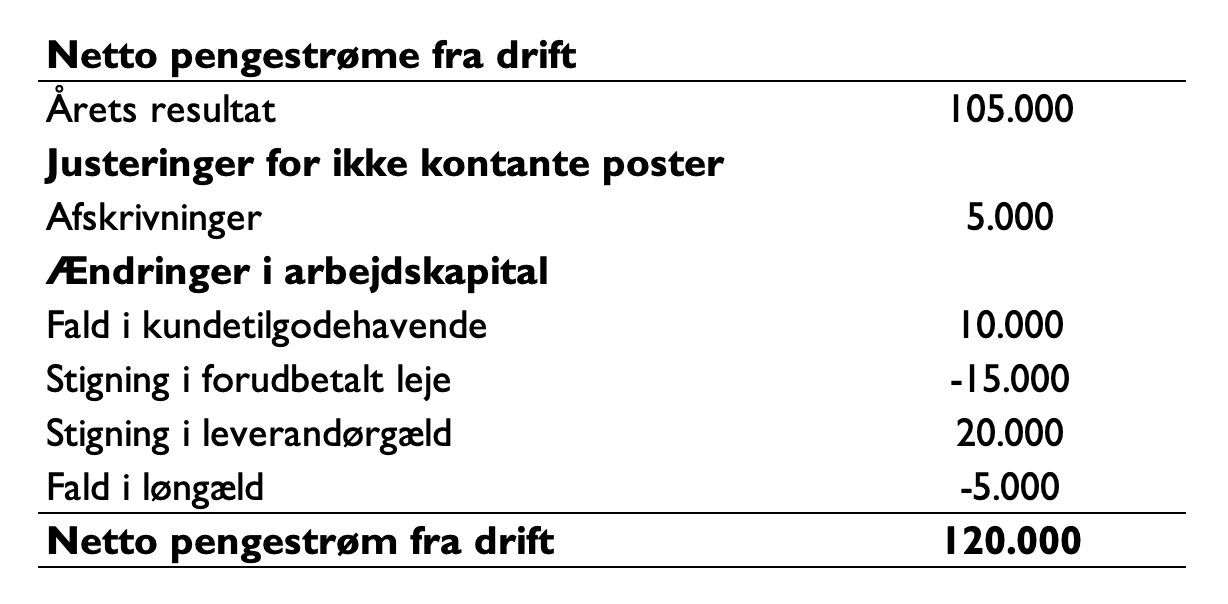
\includegraphics[scale=0.5]{pengestrømsopgørelse, indirekte.png}
     \caption{Indirekte pengestrømsopgørelse, M-karrusel}
     \label{Figur 1}
\end{figure}
Ændringerne i arbejdskapitalen skyldes da, at (1) kundetilgodehavender er faldet fra 75.000 kr. til 65.000 kr., hvilket er en indtægt på 10.000 kr, (2) forudbetalt leje er steget fra 65.000 kr. til 80.000 kr., hvilket er en udgift på 15.000 kr, (3) leverandørgæld er steget fra 80.000 kr. til 100.000 kr., hvilket er en indtægt på 20.000 kr. og (4) løngæld er faldet fra 40.000 kr. til 35.000 kr., hvilket er en udgift på 5.000 kr. Fortolkningen er i den forbindelse, at M-karrusel har et positivt cash flow på 120.000 fra deres driftsaktiviteter i 2022. Det betyder, at virksomhedens daglige driftsaktiviteter har genereret netto likvider på 120.000 kr. i løbet af året. Et positivt cash flow fra driften indikerer således, at M-karrusel er i stand til at genere tilstrækkelige kontante midler til at opretholde (og muligvis udvide) sin drift, betale sine regninger, samt afdrage evt. gæld og udbetale evt. udbytte.

\subsection{Regnskabsanalyse}
Indenfor regnskabsanalyse skelner man traditionelt set mellem nøgletal der belyser (1) virksomhedens profitabilitet, (2) virksomhedens finansielle gearing, (3) virksomhedens solvens/likviditet og (4) aktivernes omsætningshastighed i virksomheden. Beregningen af disse nøgletal tager udgangspunkt i selskabets egne regnskabsdata og er da oftest tilbageskuende (medmindre solvensgraden, m.m.). Der findes desuden en række andre nøgletal, der tager udgangspunkt i aktiemarkedet og kombinerer dette med virksomhedens interne regnskabsdata (f.eks. 'earnings per share' og 'P/E ratio'). I det følgende gennemgås alle nøgletal, samtidig med, at intuitionen bag og eksempler gennemgås. 

\subsubsection{Nøgletal for profitabilitet}
Det første, og mest intuitive nøgletal for profitabilitet er \textbf{egenkapitalens forretning} (kort EKF), der på engelsk benævnes 'return on equtiy (ROE)'. EKF defineres som: 

\begin{equation}
    \text{EKF} = \frac{\text{resultat før skat}}{\text{gns. egenkapital}}
\end{equation}

Og måler grundlæggende ejernes afkast af deres investering i virksomheden. Det bemærkes desuden, at der i brøkens nævner står gns. egenkapital, der bestemmes på baggrund af primo- og ultimoniveauer. Den gennemsnitlige egenkapital er oftest et mere retvisende tal end blot at betragte ultimoværdien, idet det er usandsynligt, at egenkapitalen har været på 'ultimo-niveau' i løbet af hele regnskabsåret. EKF bestemmes nedenfor for et selskab, der før sket havde et resultat på 10 mio., samt en primo egenkapital på 195 mio. og en ultimo egenkapital på 230 mio. Da er EKF: 

\begin{equation}
    \text{EKF} = \frac{10}{\frac{195+230}{2}} \approx 4.7 \% \nonumber
\end{equation}

En fortolkning heraf er, at for hver 100 kr. i egenkapital som ejerne investerer, vil de modtage et afkast (i form af profit før skat) på 4.7 kr. Udfordringen ved EKF som et mål for profitabilitet er dog, at det ikke tager højde for gældsfinansiering. En virksomhed med lav egenkapital (og høj gæld), vil da kunne have en langt større EKF end en tilsvarende virksomhed med det samlede antal totale passiver/aktiver, men blot en lavere gældsfinansiering (da gns. egenkapital her vil være større). 

\vspace{10 pt}

For at tage højde for gældsfinansiering benyttes \textbf{afkastningsgraden} (kort AG), der på engelsk refereres til som 'return on assets (ROA)'. AG er defineret som: 

\begin{equation}
    \text{AG}_{\text{før skat}} = \frac{\text{resultat før skat + renteudgifter}}{\text{gns. samlede aktiver}}
\end{equation}

Årsagen til, at der i tælleren står summen af resultat før skat og renteudgifter er, at denne sum netop indeholder det samlede afkast til virksomhedens investorer (resultat til ejerne, renteudgifter til virksomhedens kreditorer). Brøkens nævner udtrykker den totale kapital investeret i virksomheden og kan erstattes af passiver, hvis man ønsker det. Afkastningsgraden udtrykker således forrentningen af virksomhedens samlede investerede kapital. Bemærk, at hvis der er tale om 'efter-skat' beregninger, bliver formlen: 

\begin{equation}
    \text{AG}_{\text{efter skat}} = \frac{\text{resultat efter skat + renteudgifter} \cdot (1 - \text{skatterate})}{\text{gns. samlede aktiver}}
\end{equation}

Hvis virksomheden fra eksemplet ovenfor har en gns. gæld på 750 mio, vil AG da være: 

\begin{equation}
    \text{AG} = \frac{10}{212.5 + 750} \approx 1.04 \% \nonumber
\end{equation}

Som er et langt mindre tilfredsstillende resultat end ovenstående. Et intuitivt eksempel, der viser vigtigheden af følsomheden af EKF overfor gældsfinansiering i særligt investeringsprojekter er givet nedenfor: 


\begin{tcolorbox}[colback=red!5!white, colframe=red!50!black, title=Gældsfinansiering og EKF/AG, breakable]
Betragt følgende investeringsprojekt: 

\begin{itemize}
    \item Krævet kapital: 1.800 mio.
    \item Afkast med 80 \% sandsynlighed: 300 mio. 
    \item Afkast med 20 \% sandsynlighed: -300 mio. 
\end{itemize}

Hvis virksomheden finansierer projektet med 100 pct. egenkapital, vil ROE med 80 pct. sandsynlighed være: 
 \begin{equation}
     \text{EKF}_\text{80 pct.} = \frac{300}{1.800} \approx 16.6 \% \nonumber
 \end{equation}

Og tilsvarende med 20 pct.: 

 \begin{equation}
     \text{EKF}_\text{20 pct.} = -\frac{300}{1.800} \approx -16.6 \% \nonumber
 \end{equation}

Hvis selskabet i stedet vælger at finansiere projektet med halv gældsfinansiering og optager et lån på 900.000 med 5 pct. rente bliver EKF med 80 pct. sandsynlighed: 

 \begin{equation}
     \text{EKF}_\text{80 pct., gældsfinansiering 50 pct.} = -\frac{300-900\cdot0.05}{900} \approx 28.3 \% \nonumber
 \end{equation}

Og tilsvarende med 20 pct. sandsynlighed: 

 \begin{equation}
     \text{EKF}_\text{20 pct., gældsfinansiering 50 pct.} = -\frac{-300-900\cdot0.05}{900} \approx -38.3 \% \nonumber
 \end{equation}

 Med 80 pct. gældsfinansiering bliver EKF yderligere påvirket. Med 80 pct. sandsynligheden er EKF  da: 

\begin{equation}
     \text{EKF}_\text{80 pct., gældsfinansiering 80 pct.} = -\frac{300-1440\cdot0.05}{360} \approx 63.3 \% \nonumber
 \end{equation}

 Og tilsvarende med 20 pct. sandsynlighed: 

 \begin{equation}
     \text{EKF}_\text{20 pct., gældsfinansiering 80 pct.} = -\frac{-300-1440\cdot0.05}{360} \approx -103 \% \nonumber
 \end{equation}

\tikz[baseline=(X.base)] 
\node [draw=red, thick, rectangle, text width=.99\linewidth] (X) {$\implies$ EKF er sensitivt overfor ændringer i gældsfinansiering, hvilket er en begrænsning af målet.};

\vspace{10 pt}

Ved brug af AG kan selv samme investeringsprojekt analyseres, hvor ændringer i gældsfinansiering ikke spiller nogen rolle. Da: 
\begin{align}
    \text{AG}_\text{80 pct., gældsfinansiering 0 pct.} & = \frac{300}{1800} \approx 16.6 \nonumber \\
    \text{AG}_\text{20 pct., gældsfinansiering 0 pct.} & = \frac{-300}{1800} \approx -16.6 \nonumber \\
    \text{AG}_\text{80 pct., gældsfinansiering 50 pct.} & = \frac{300-900\cdot0.5 + 900\cdot0.5 }{1800} \approx 16.6 \nonumber \\
    \text{AG}_\text{80 pct., gældsfinansiering 50 pct.} & = \frac{-300-900\cdot0.5 + 900\cdot0.5 }{1800} \approx -16.6 \nonumber \\
    \text{AG}_\text{80 pct., gældsfinansiering 80 pct.} & = \frac{300-1440\cdot0.5 + 1440\cdot0.5 }{1800} \approx 16.6 \nonumber \\
    \text{AG}_\text{20 pct., gældsfinansiering 80 pct.} & = \frac{-300-900\cdot0.5 + 900\cdot0.5 }{1800} \approx -16.6 \nonumber
\end{align}

\tikz[baseline=(X.base)] 
\node [draw=red, thick, rectangle, text width=.99\linewidth] (X) {$\implies$ Ved at betragte AG i stedet for EKF kan man sikre sin analyse overfor ændringer i gældsfinansiering.};

\end{tcolorbox}

Et sidste mål for profitabiliteten er \textbf{overskudgraden} (OG), der på engelsk benævnes 'return on sales (ROS)'. Målet er et udtryk for, hvor effektivt en virksomhed konverterer omsætning til profit. Det er dog værd at understrege, at sammenligninger med overskudgrad kun er hensigtsmæssige, hvis der er tale om virksomheder indenfor lignende brancher og disse er af lignende størrelse. OG er defineret som: 

\begin{equation}
    \text{Overskudsgrad} = \frac{\text{resultat + renteudgifter}}{\text{omsætning}}
\end{equation}

Overskudsgraden angiver da, hvor stor en andel af en krones salg, der i \textit{gennemsnit} tilfalder virksomhedens investorer, her defineret som ejere og kreditorer. Betragt f.eks. en virksomhed med 210 mio. i resultat, 30 mio. i renteudgifter og 1200 mio. i omsætning. Da gælder: 

\begin{equation}
    \text{Overskudsgrad} = \frac{210+30}{1200} = 20 \% \nonumber
\end{equation}

Altså vil en krones salg i virksomheden i gennemsnit tilfalde virksomhedens investorer med 20 øre. 

\vspace{1.5 pt}

\hspace{5 pt} Det gælder generelt, at en virksomhed godt kan have en høj overskudsgrad, samtidig med, at forretningen af egenkapitalen er lav, hvis virksomheden sælger få, men dyre enheder (som de tjener meget på). Samtidig kan en virksomheden også have en lav overskudsgrad, men en høj forretning af egenkapitalen, hvis virksomheden sælger mange billige enheder, som virksomheden per styk ikke tjener synderlig meget på (svarende til høj omsætningshastighed). 

\vspace{10 pt}

Desuden vil en negativ overskudsgrad ikke nødvendigvis medføre, at virksomhedens ejere vil være bedre stillet ved at stoppe salget. Det skyldes, at der kan være store, faste, etableringsomkostninger (sunk cost), der medfører, at selskabet mindsker deres tab ved fortsat at sælge enheder. Det gælder generelt, at en virksomhed skal blive ved med at sælge enheder, så længe den har et strengt positivt dækningsbidrag, dvs. $C = P - V > 0$, hvor $C$ betegner dækningsbidraget, $P$ er et udtryk for omsætningen og $V$ betegner de variable omkostninger ved produktionen af godet. 

\subsubsection{Nøgletal for finansiel gearing}
Nøgletallene for finansiel gearing beskriver i hvor høj grad virksomheder benytter ekstern finansiering til driften. Det første mål beskriver således gældens andel af den samlede kapital og benævnes \textbf{gearing i kapitalstrukturen} (GIK), eller engelsk: 'capital structure leverage' og er defineret som: 

\begin{equation}
    \text{Gearing i kapitalstrukturen} = \frac{\text{gns. samlede aktiver}}{\text{gns. egenkapital}}
\end{equation}

hvor $\text{samlede aktiver} = \text{egenkapital} + \text{gæld}$. Nøgletallet beskriver således, hvor stor en del af de samlede aktiver, der ejes af virksomhedens ejere (gennem egenkapital) og hvor stor en del, der er finansieret gennem fremmedkapital. En højere værdi af GIK er da et udtryk for mere gældsfinansiering og det gælder generelt, at $\text{GIK} \ge 1$, idet de samlede aktiver ellers skulle være mindre end egenkapitalen. For en virksomhed med samlede aktiver på 500 mio. og egenkapital på 100 mio, vil GIK være: 

\begin{equation}
    \text{Gearing i kapitalstrukturen} = \frac{500}{100} = 5 \nonumber
\end{equation}

Fortolkningen heraf er, at for hver enhed af egenkapital finansierer virksomheden 5 enheder af aktiver, svarende til en høj gældsfinansiering ift. egenkapitalsfinansiering. 

\vspace{10 pt}

En anden måde at beskrive GIK på er gennem \textbf{gæld-egenkapital forholdet}, der er defineret som: 

\begin{equation}
    \text{gæld-egenkapital forholdet} = \frac{\text{gns. gæld}}{\text{gns. egenkapital}}
\end{equation}

Hvis f.eks. GIK er lig 10, må gæld-egenkapital forholdet være lig: 
\begin{align}
\centering
     10 & = \frac{\text{egenkapital}}{\text{egenkapital}} + \frac{\text{gæld}}{\text{egenkapital}} \nonumber \\
     10 & = 1 + \frac{\text{gæld}}{\text{egenkapital}} \nonumber \\
     9 & = \frac{\text{gæld}}{\text{egenkapital}} \nonumber
\end{align}

Et andet nøgletal for en virksomheds finansielle gearing, er \textbf{gearing i indkomststrukturen} (GIS), der på engelsk benævnes 'common equity leverage' og beskriver renteudgifternes andel af indtjeningen. GIS er da lig: 

\begin{equation}
        \text{Gearing i indkomststruktur} = \frac{\text{resultat}}{\text{resultat + renteudgifter}}
\end{equation}

Og beskriver, hvor stor en andel af det samlede overskud, der tilfalder virksomhedens ejere (i modsætning til kreditorerne). Et høj værdi af nøgletallet indikerer her en lav gearing (svarende til, at en stor del overskuddet tilfalder ejerne). Målet er følsomt overfor virksomhedens profitabilitet. Betragt f.eks. en virksomhed med et resultat på 10 mio. og renteudgifter for 2 mio., her vil GIS være lig: 

\begin{equation}
        \text{Gearing i indkomststruktur} = \frac{10}{10+2} \approx 83.3 \% \nonumber 
\end{equation}

Svarende til, at 83.3 pct. af overskuddet går til ejerne, mens $1-0.833$ går til aflønning af kapital (til kreditorerne). Målet kan desuden omskrives til: 

\begin{equation}
        \frac{1}{\text{Gearing i indkomststruktur}} = 1 + \frac{\text{renteudgifter}}{\text{resultat}}
\end{equation}

Dvs. 

\begin{equation}
        \frac{1}{\text{Gearing i indkomststruktur}} = 1 + \frac{2}{10} = 1.2 \nonumber
\end{equation}

\subsubsection{Nøgletal for solvens og likviditet}
Nøgletal for solvens beskriver, hvor store værdier virksomheden har på \textit{kistebunden}, og er dermed afgørende for potentielle kreditorer, der skal afgøre, hvorvidt de vil låne virksomheden penge/levere varer på kredit. Likviditet refererer derimod til virksomhedens evne til at opfylde sine kortsigtede økonomiske forpligtelser, dvs. dens evne til hurtigt at omdanne aktiver til kontanter uden et betydeligt tab af værdi. Solvens/likvditetsmål hidrører enten (1) aktiver, der kan realiseres ift. gæld, der forfalder og er da baseret på balancen eller (2) indkomst i forhold til udgifter (baseret på resultatopgørelsen).  

\vspace{10 pt}

\textbf{Likvididetsgrad A}, på engelsk benævnt 'current ratio', udtrykker da hvor mange aktiver, der kan omsættes indenfor et år i forhold til den mængde gæld, der forfalder indenfor samme år. Altså:

\begin{equation}
    \text{Likviditetsgrad A} =  \frac{\text{omsætningsaktiver}}{\text{kortfristet gæld}}
\end{equation}

En virksomhed med omsætningsaktiver for 5 mio. og kortfristet gæld på 1 mio., vil da have en likviditetsgrad på 5, svarende til, at omsætningsaktiverne kan betale værdien af den kortfristede gæld 5 gange. Selv hvis nøgletallet er mindre end 1 betyder det dog ikke, at virksomheden vil gå konkurs. Det vil blot kræve en omlægning af finansiering, samt/eller mere kontant salg. 

\vspace{10 pt}

\textbf{Likvididetsgrad B}, på engelsk benævnt 'quick ratio', er nært beslægtet, men mere snævert og beskriver da, hvor mange aktiver, der kan realiseres til kontanter i forhold til gæld, der forfalder indenfor et år. Da: 

\begin{equation}
    \text{Likviditetsgrad B} =  \frac{\text{kontanter + værdipapirer + tilgodehavender}}{\text{kortfristet gæld}}
\end{equation}

En virksomhed med kontanter til 1 mio., værdipapirer til 3 mio. og tilgodehavender til 5 mio., samt kortfristet gæld til 10 mio. vil da have en quick ratio på: 0.9, svarende til, at salget af disse tre aktiver alene ikke vil kunne dække virksomhedens kortfristede gældsforpligtelser. 

\vspace{10 pt}

\textbf{Rentedækningsratioen}, på engelsk 'interest coverage' (IC),  udtrykker overskuddet, der kan bruges til rentebetalinger i forhold til de faktiske rentebetalinger. Altså: 

\begin{equation}
    \text{Rentedækningsratio} =  \frac{\text{resultat + renteomkostninger + skat}}{\text{renteomkostninger }}
\end{equation}

Årsagen til, at skat indgår i tælleren er, at rentebetalinger er fradragsberettiget og rentebetalingerne da afholdes før der betales skat. IC bør være noget større end 1, dvs. der bør generes et tilstrækkeligt overskud til at dække løbende renteomkostninger. Selv hvis IC er langt større end 1, kan der dog opstå likviditetsproblemer, hvis f.eks. en langsigtet gældspost forfalder. Samtidig vil en IC på under 1 ikke nødvendigvis være et likviditetsproblem, idet renteomkostningerne kan betales via en kontantbeholdning. En virksomhed med et resultat på 5 mio., renteomkostnigner for 1 mio. og skat for 1 mio. vil da have en IC på 7, svarende til, at virksomheden vil kunne betale renteomkostningerne 7 gange med det tilgængelige overskud. 

\vspace{10 pt}

Generelt kan man sige, at de to likviditetsmål er fremadskudende, mens IC er tilbageskuende. En langsigtet gældspost, der forfalder i den kommende periode vil således kun påvirke likvidietsgrad A og B, under antagelse af, at renteomkostningerne ikke ændrer sig.  

\subsubsection{Nøgletal for aktivernes omsætningshastighed}
\textbf{Aktivernes omsætningshastighed}, på engelsk 'total asset turnover', udtrykker hvor hurtigt virksomhedens aktiver i gennemsnit bliver omsat til salg. Dvs: 

\begin{equation}
    \text{Aktivernes omsætningshastighed} =  \frac{\text{omsætning}}{\text{gns. samlede aktiver}}
\end{equation}

Hermed beskriver nøgletallet, hvor meget salg der generes per krone kapital investeret i virksomheden. Betragt f.eks. en virksomhed med aktiver på 12.000 og en omsætning på 100.000. Heraf kan det sluttes, at aktiverne i gennemsnit omsættes 8.3 gange om året, svarende til ca. en gang hver 44 dag ($\frac{365}{8.3}$). Det er således muligt at kombinere en lav overskudsgrad med en høj forrentning af egenkapitalen, hvis der f.eks. er en høj omsætningshastighed. 

\vspace{10 pt}
\textbf{Tilgodehavenders omsætningshatighed}, på engelsk 'receivables turnover', beskriver, hvor effektiv virksomheden er til at realisere kundetilgodehavender og bestemmes som: 

\begin{equation}
    \text{Tilgodehavenders omsætningshastighed} =  \frac{\text{salg på kredit}}{\text{gns. kundetilgodehavender}}
\end{equation}

Betragt f.eks. en virksomhed med et samlet salg på kredit på 5000 og kundetilgodehavender på 1000, heraf følger det, at virksomheden har indsamlet sin gennemsnitlige debitorsaldo 5 gange i løbet af den periode, der måles. Altså: den samlede sum af kreditværdier, virksomheden har solgt og efterfølgende indsamlet betaling for, er 5 gange større end den gennemsnitlige mængde af udeståender (kundetilgodehavender) på ethvert givent tidspunkt i løbet af perioden. Med andre ord, bliver hver krone af kundetilgodehavender i gennemsnit indsamlet og omdannet til kontanter 5 gange om året.

\vspace{10 pt}
\textbf{Lagerets omsætningshatighed}, på engelsk 'inventory turnover', beskriver afslutningsvis, hvor langt tid det i gennemsnit taget at få \textit{tømt} lageret og er defineret som: 

\begin{equation}
    \text{Lagerets omsætningshastighed} =  \frac{\text{vareforbrug}}{\text{gns. varelager}}
\end{equation}

Bemærk, at vareforbruget kommer fra resultatopgørelsen, mens varelagerværdierne kommer fra balancen. Har en virksomhed haft vareforbrug på 80.000 og et varelager på 20.000, er lagerets omsætningshastighed lig 4, svarende til, at virksomheden har solgt og erstattet sit lager 4 gange i løbet af regnskabsperioden. En høj omsætningshastighed er her, alt andet lige, positivt idet det det vidner om, at relativt lidt kapital er bundet tilgodehavender/varelager. 

\subsubsection{Andre nøgletal}
De øvrige nøgletal, der ikke tager udgangspunkt i virksomhedens interne regnskabsdata, benævnes \textit{andre nøgletal}. Det første nøgletal i den henseende er \textbf{resultat per aktie}, på engelsk 'earnings per share', og er defineret som: 

\begin{equation}
    \text{Resultat per aktie} =  \frac{\text{resultat efter skat}}{\text{antal udstedte aktier}}
\end{equation}

Nøgletallet er dermed et udtryk for det overskud, der tilfalder hver aktie (enten som dividende eller henlagt overskud). Betragt f.eks. en virksomhed, der har et resultat på 1000 mio efter skat og har udstedt 100 mio. aktier. Her vil resultatet per aktie vær lig 10. Tallet i sig selv er dog ikke synderlig informativt, idet aktiens markedspris (der for aktionæren repræsenterer en investering), bør medtages for at bestemme, hvorvidt det nominelle afkast er tilfredsstillende. Koster aktien i eksemplet ovenfor 100 kr. er afkastet tilfredsstillende, men erhverves den i stedet for 1000, er det ikke længere tilfældet. 

\vspace{10 pt}
\textbf{Price-earnings ratio}, kort 'P/E', tager højde for markedsprisen ved at beskrive forholdet mellem markedsprisen per aktie og resultatet per aktie. Dvs: 

\begin{equation}
    \text{Price-earnings ratio} =  \frac{\text{markedspris per aktie}}{\frac{\text{resultat efter skat}}{\text{antal udstedte aktier}}} = \frac{\text{markedspris per aktie}}{\text{resultat per aktie}}
\end{equation}

P/E udtrykker således hvor meget en potentiel investor skal betale for en krones overskud i denne og hver af alle fremtidige perioder. En lav P/E betyder, at man kan nyde godt af en fremtidig indkomststrøm billigt (oftest fordi markedet forventer, at virksomheden/markedet stagnerer eller går tilbage), mens en høj P/E er et udtryk for, at markedet tror på fremtiden af virksomheden. Betragt eksemplet ovenfor, hvor resultatet per aktie var 10 og markedsprisen f.eks. er 100. Her er P/E 10, svarende til, at en nutidig investor skal betale $10X$ resultatet per aktie for at få en del af virksomhedens overskud. 

\vspace{10 pt}

\textbf{Aktieafkastet}, på engelsk 'stock price return', er et udtryk for det markedsmæssige afkast til aktionærerne og defineres som: 

\begin{equation}
    \text{Aktieafkast} = \frac{\text{aktiekurs}_1 - \text{aktiekurs}_0 + \text{udbytte}_1}{\text{aktiekurs}_0}
\end{equation}

Det markedsmæssige afkast består da af to dele: (1) kursgevinsten (stigningen i aktiens markedspris) og (2) udbytte. Det bemærkes, at der er tale om et faktisk aktieafkast, fordi det kan realiseres ved salg af aktien på tidspunkt 1. Betragt en aktie, der til tidspunkt 1 havde en pris 100 og på tidspunkt 0 havde en pris på 75. Dertil kommer, at der er blevet udbetalt udbytte af størrelsen 15 på tidspunkt 1. Aktieafkastet er da: 

\begin{equation}
    \text{Aktieafkast} = \frac{100-75+15}{\text{75}} \approx 53.3 \% \nonumber
\end{equation}


\subsubsection{Dekomponering af EKF}
Dekomponering af egenkapitalens forrentning kan grundlæggende bruges til at besvare to spørgsmål: 
\begin{enumerate}
    \item Hvad driver forbedringer/forværringer i EKF over tid (i samme virksomhed)?
    \item Hvad forklarer forskelle i EKF mellem virksomheder i samme branche?
\end{enumerate}

Egenkapitalen kan da dekomponeres til fire forskellige \textit{key drivers}, hvor det gælder: 

\begin{equation}
    \text{EKF} =  \underbrace{\frac{\text{resultat}}{\text{(resultat + renter)}}}_{\text{GIS}} \cdot \underbrace{\frac{\text{(resultat + renter)}}{\text{omsætning}}}_{\text{Overskudsgrad}} \cdot \underbrace{\frac{\text{omsætning}}{\text{gns. aktiver}}}_{\text{Akt. oms. hastighed}} \cdot \underbrace{\frac{\text{gns. aktiver}}{\text{gns. egenkapital}} }_{\text{GIK}}
\end{equation}

Egenkapitalens forrentning kan altså skrives vha. fire andre nøgletal: GIS, OG, akt. omsætningshastighed og GIK. EKF drives da:

\vspace{10 pt}

(1) af virksomhedens overskudsgrad ($\frac{\text{(resultat + renter)}}{\text{omsætning}}$), dvs. hvor god virksomheden er til at genere overskud af sit salg. Dette mål beskriver, groft sagt, driftsfunktionen i selskabet, dvs. salgarbejde og omkostningsstyring. 

\vspace{10 pt}

(2) af aktivernes omsætningshastighed ($\frac{\text{omsætning}}{\text{gns. aktiver}}$), dvs. hvor god virksomheden er til at skabe salg ved hjælp af den investerede kapital. Dette mål beskriver, groft sagt, investeringsfunktionen i selskabet ('long-term asset management') 

\vspace{10 pt}

(3) af virksomhedens gearing ($\text{GIS} \cdot \text{GIK}$), dvs. hvor god virksomheden er til at bruge fremmedkapital til at øge overskuddet. Det kan være kontraintuitivt at medtage gearing (GIK og GIS) i EKF-dekomponeringen, da EKF netop fokuserer på egenkapitalen og ikke på virksomhedens gæld. Alligevel medtages det, da virksomhedens kapitalstruktur – forholdet mellem gæld og egenkapital – netop påvirker rentabiliteten af egenkapitalen. Denne del af EKF dekomponeringen beskriver da, groft sagt, selskabets finansieringsevne ('capital structure management') 

\begin{tcolorbox}[colback=red!5!white, colframe=red!50!black, title= Eksempel af EKF dekomponering, breakable]
Betragt følgende nøgletal for virksomhed A: 

\begin{itemize}
    \item Resultat før renter (Resultat): 2.000.000 DKK
    \item Renter: 150.000 DKK
    \item Omsætning: 10.000.000 DKK 
    \item Gennemsnitlige aktiver (gns. aktiver): 12.000.000 DKK
    \item Gennemsnitlig egenkapital (gns. egenkapital): 4.000.000 DKK
\end{itemize}

Egenkapitalens forrentning er lig: 

\begin{equation}
    \text{EKF} = \frac{2.000.000}{4.000.000} = 50 \% \nonumber
\end{equation}

Som kan dekomponeres til: 

\begin{align}
    \text{EKF} & = \frac{2.000.000}{2.150.000} \cdot \frac{2.150.000}{10.000.000} \cdot \frac{10.000.000}{12.000.000} \cdot \frac{12.000.000}{4.000.000} \\
    \text{EKF} & = 0.93 \cdot 0.215 \cdot 0.83 \cdot 3 \approx 50 \% \nonumber
\end{align}

Heraf følger: 

\begin{itemize}
    \item GIS: Værdien 0.930 viser, at en stor del af virksomhedens overskud efter skat kommer fra dens drift og ikke er væsentligt forøget af finansielle omkostninger. En værdi tæt på 1 indikerer, at renteomkostninger ikke har en stor negativ indflydelse på virksomhedens rentabilitet.
  \item Overskudsgrad: Denne margin fortæller, hvor meget virksomheden tjener, efter alle omkostninger er betalt, for hver krone af omsætning. En overskudsgrad på 21.5 pct. betyder, at for hver krone virksomheden tjener, bliver 0.215 krone tilbage som overskud efter renter. Det er en sund margin og indikerer god rentabilitet på salget.
\item Aktivernes omsætningshastighed (83.3 pct.): Dette indikerer, hvor effektivt virksomheden bruger sine aktiver til at generere omsætning. En omsætningshastighed på 83.3 pct. indikerer, at for hver krone i aktiver, genererer virksomheden ca. 0.83 krone i omsætning. Dette tal kan betragtes som moderat og indikerer, at der er plads til forbedring i aktivudnyttelsen.
\item GIK (Gældens indflydelse på kapitalforrentningen): Værdien 3.0 viser forholdet mellem de samlede aktiver og egenkapitalen. En GIK på 3.0 indikerer, at virksomheden har tre gange så mange aktiver som egenkapital, hvilket kan tyde på en høj gældsgrad. Dette kan øge risikoen, men også potentialet for højere afkast, hvis aktiverne forrenter sig bedre end omkostningen ved gælden.
\end{itemize}
\end{tcolorbox}

\subsubsection{Dekomponering af gearing i EKF}
Produktet af de to faktorer, der udtrykker gearing i EKF dekomponeringen (GIS og GIK), kan omskrives til, hvor AG = afkastningsgraden:  

\begin{equation}
    \left( 1 + \frac{\text{gæld}}{\text{egenkapital}} \right)
\left( \frac{\frac{\text{resultat}+\text{renter}}{\text{aktiver}} - \frac{\text{renter}}{\text{gæld}}}
             {\frac{\text{resultat}+\text{renter}}{\text{aktiver}}} \right)
= \left( 1 + \frac{\text{gæld}}{\text{egenkapital}} \right)
\left( \frac{\text{AG} - \frac{\text{renter}}{\text{gæld}}}{\text{AG}} \right)
\end{equation}

Heraf følger, at gearingen har ingen effekt på EKF, hvis gælden er nul, da hele udtrykker så er lig 1. Det gælder desuden, at:

\begin{itemize}
    \item EKF vil forøges ved yderligere gæld, hvis $\text{AG} > \frac{\text{renter}}{\text{gæld}}$
    \item EKF vil fale ved mere gæld, hvis $\text{AG} < \frac{\text{renter}}{\text{gæld}}$
\end{itemize}

Intuitionen er her, at gæld øger egenkapitalens forrentning, hvis virksomhedens investeringer (AG) i gennemsnit har et højere afkast end lånerenten. 


\begin{tcolorbox}[colback=red!5!white, colframe=red!50!black, title= Eksempel af EKF dekomponering, breakable]
Antag, at virksomhed A har en lånerente på 1.25 pct (8.000.000 i gæld og 150.00 i renteudgifter) og en afkastningsgrad på: $\frac{2.150.000}{12.000.000} \approx 17.9$. Her vil det gælde, at: 

\begin{equation}
    (1 + \frac{8.000.000}{4.000.000} \cdot (\frac{0.179 - 0.0125}{0.179})
\end{equation}

Da $\text{AG} > \text{lånerenten}$, gælder det, at virksomheden kan øge EKF ved at optage mere gæld... 
\end{tcolorbox}

\subsubsection{Opsamling}
Afsnit 1.4 har da beskrevet og gennemgået de mest gængse mål for regnskabsanalyse. Indenfor profitabilitet operer man med begreberne: \textbf{egenkapitalens forrentning (EKF)}, \textbf{afkastningsgrad (AG)}, og \textbf{overskudsgrad (OG)}. 

\vspace{10 pt}

Til beskrivelse af finansiel gearing benyttes: \textbf{gearing i kapitalstruktur (GIK)}, \textbf{gæld-egenkapital forholdet} og \textbf{gæld i indkomststruktur (GIS)}. 

\vspace{10 pt}

Ved analyse af solvens/likviditet betragtes: \textbf{likviditetsgrad A}, \textbf{likviditetsgrad B} og \textbf{rentedækningsratioen}, hvor de første to er fremadskudende, hvilket er forholdsvis unikt og ikke gælder andre mål i sektion 1.4. 

\vspace{10 pt}

Omsætningshastigheden af diverse aktiver vurderes ved: \textbf{aktiverne omsætningshastighed}, \textbf{tilgodehavenders omsætningshastighed} og \textbf{lagerets omsætningshastighed}. 

\vspace{10 pt}

Afslutningsvis er de øvrige mål (eksterne) givet ved: \textbf{resultat per aktie}, \textbf{P/E ratio} og \textbf{aktieafkast}.

\begin{figure}[h]
     \centering
     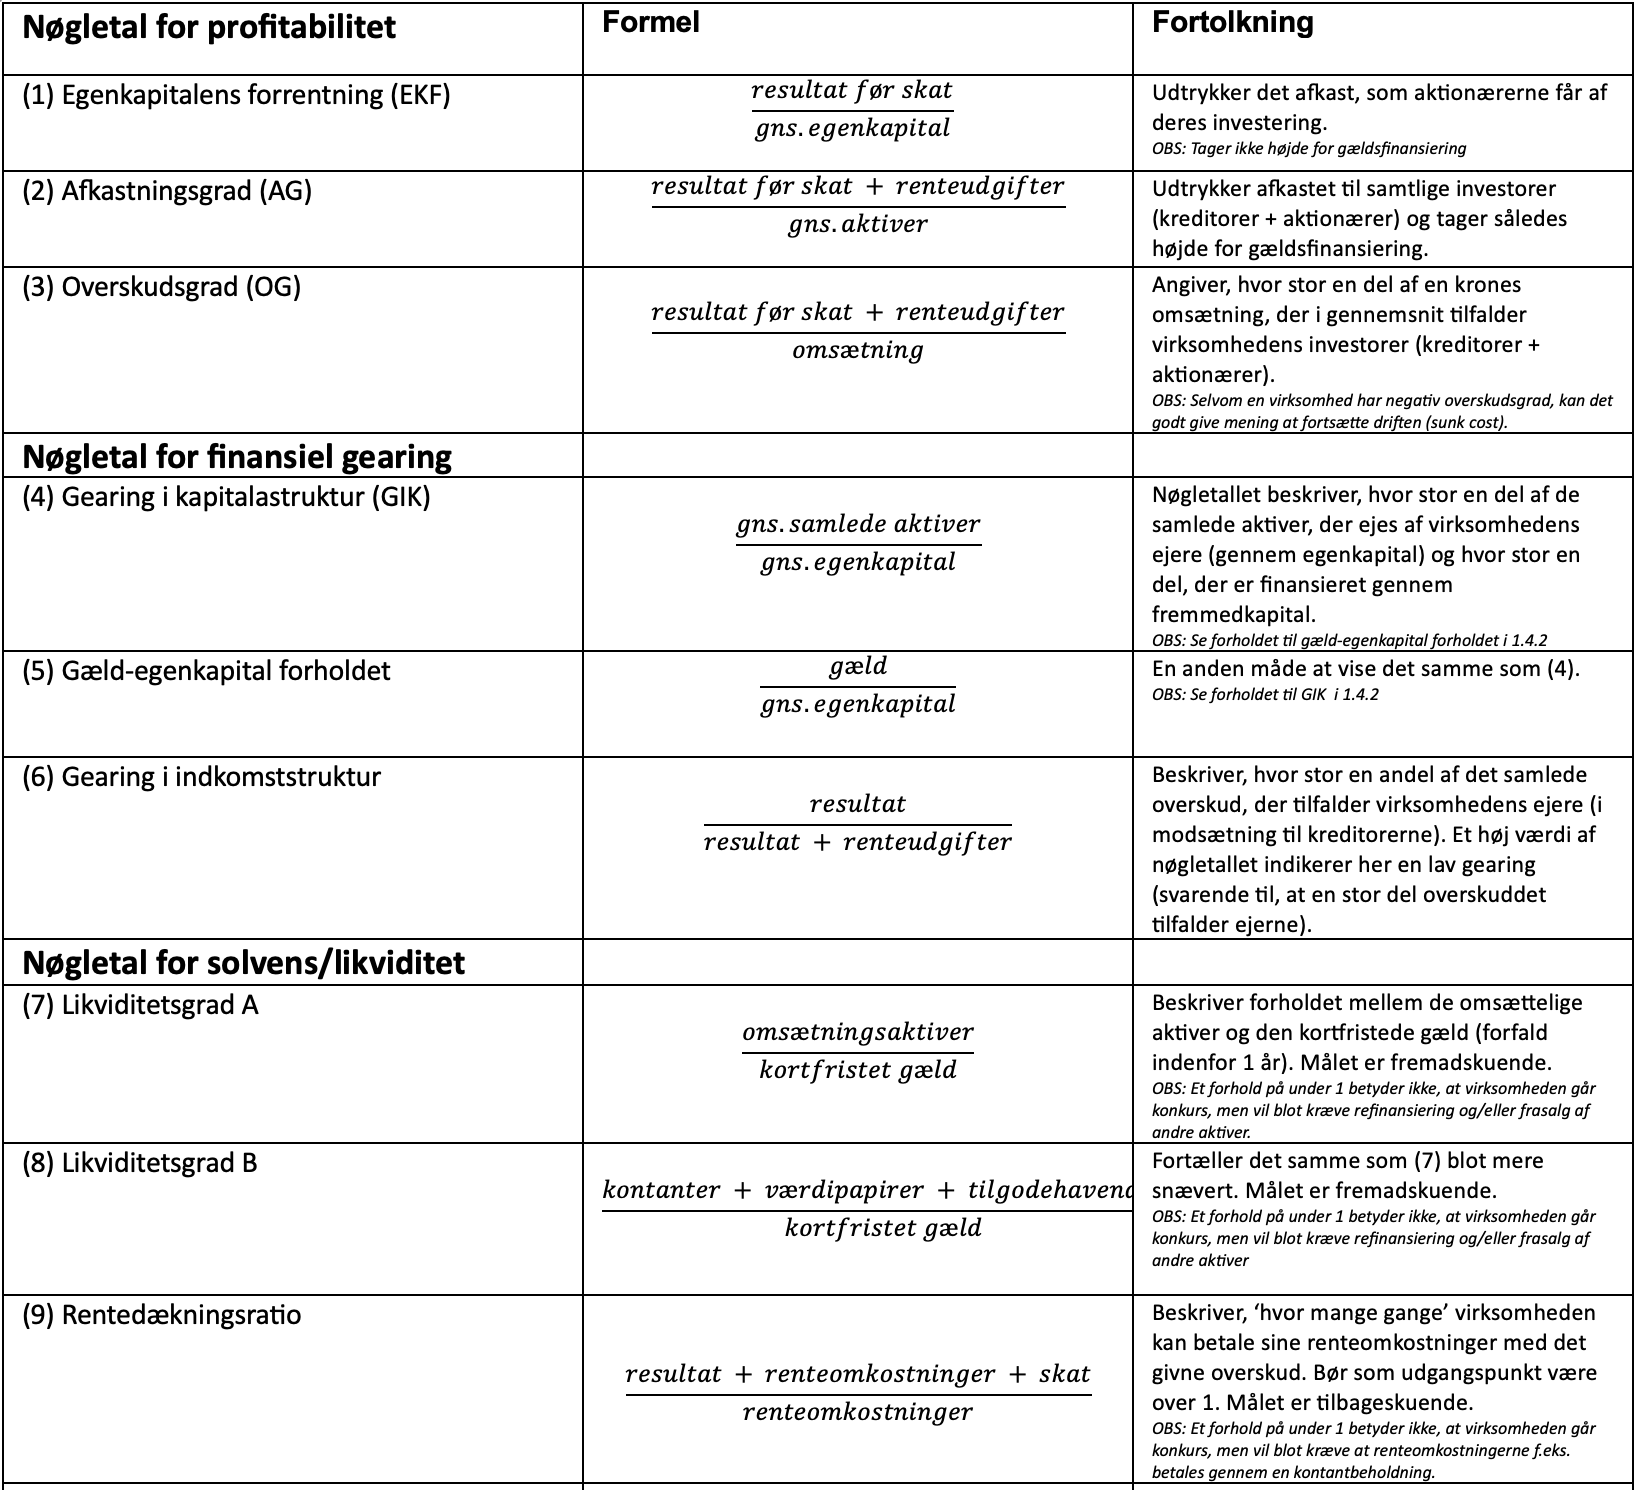
\includegraphics[scale=0.5]{oversigt 1.png}
     \caption{Vigtige nøgletal (1)}
     \label{Figur 1}
\end{figure} 

\newpage

\begin{figure}[h]
     \centering
     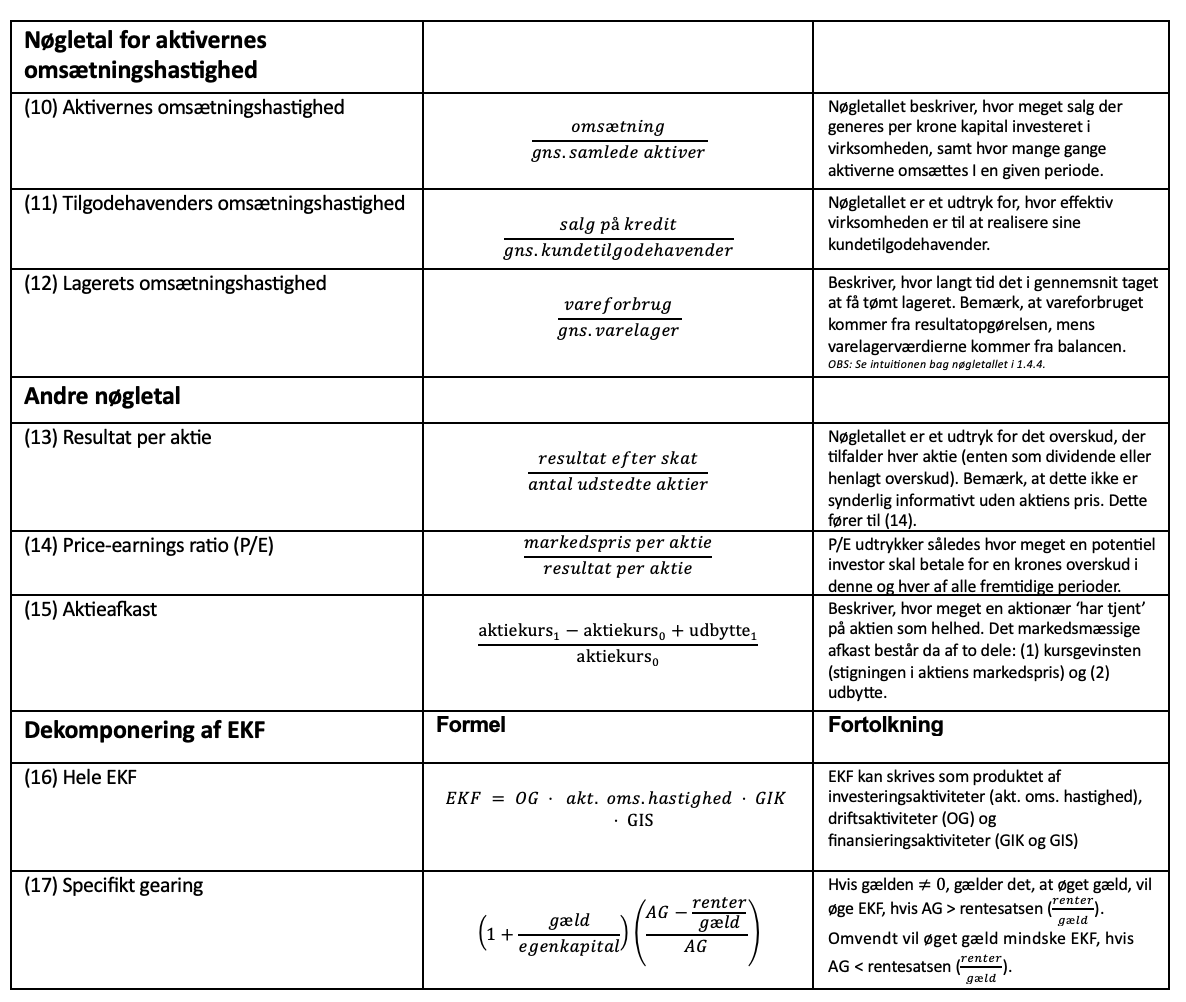
\includegraphics[scale=0.75]{oversigt 2.png}
     \caption{Vigtige nøgletal (2)}
     \label{Figur 1}
\end{figure} 

\section{Den grundlæggende matematik bag diskontering}
Investeringsteori beskriver grundlæggende virksomhedens perspektiv i en beslutning om, hvilke anlægsinvesteringer den skal foretage sig. Det kan f.eks. være investeringer i et nyt produktionsapparat, udvikling af et nyt produkt eller, hvorvidt det offentlige — i BMT delen af emnet — bør købe en ny bro eller en ny motorvej. Formålet med investeringsteori er således at beskrive, hvilke investeringer en given virksomhed (eller stat) bør gennemføre under nogle forudsætninger som f.eks. krav til afkast, tidshorisont, m.m. I hele afsnittet antages \textbf{fuldstændig sikkerhed omkring fremtide cashflows}, hvilket ikke er en helt uproblematisk antagelse, men alligevel vil give nogle brugbare resultater. Om anlægsinvesteringer gælder følgende helt grundlæggende sammenhænge: 

\begin{itemize}
    \item \textbf{Negative} betalinger hidrører fra selve investeringer og eventuelle løbende omkostninger. 
    \item \textbf{Positive} betalinger hidrører fra de løbende indtægter forbundet med investeringer, f.eks. produktionsværdien af goder, der producerer med et givent (nyt) produktionsapparat. 
    \item Det antages at, \textbf{periode 0 er nu} med mindre andet (eksplicit) angives i en opgavetekst. 
\end{itemize}

\subsection{Introduktion til \textit{Time value of money}}
I investering operer man med den grundlæggende præmis om, at penge i dag er mere værd end penge i fremtiden. I pensum gives tre forklaringer herpå: 
\begin{itemize}
    \item Kompensation for udskydelse af forbrug.
    \item Penge mister værdi som følge af inflation.
    \item Risiko for statsbankerot.
    \item Risiko for eget dødsfald.
\end{itemize}

\textbf{Fremtidsværdien} af $X$-kroner nu investeret til en rente $r$ i $t$ perioder er givet ved: 

\begin{equation}
    FV = X (1+r)^t
\end{equation}

hvor $(1+r)^t$ kaldes fremtidsværdifaktoren og udtrykket stiger eksponentielt som følge af renters rente effekten. Fremtidsværdien af 1000 kr. investeret i 50 år til en rente på 10 pct. bliver således: 

\begin{equation*}
    FV_{1000} = 1000 \cdot (1+0,1)^{50} \approx 117.390
\end{equation*}

\textbf{Nutidsværdien} er tæt beslægtet med fremtidsværdien men beskriver i stedet, hvor meget en krone investeret i $t$ år er værd i dag. Formlen for at beregne nutidsværdien er givet ved: 

\begin{equation}
    PV = X \cdot \frac{1}{(1+r)^t}
\end{equation}

hvor $X$ beskriver den samlede sum penge, der forventes at blive modtaget i fremtiden og $PV$ beskriver den nuværende værdi af $X$, diskonteret med renten $r$ i $t$ perioder (år). Det gælder, at $\frac{1}{(1+r)^t}$ kaldes diskonteringsfaktoren og $r$ kaldes diskonteringsrenten. Denne udledes på baggrund af teorier indenfor finansiering vha. CAPM og er oftest givet i eksamensopgaver. Det gælder, at jo højere diskonteringsrenten er, jo mindre er det fremtidige beløb værd i dag. Ved hjælp af formel 24 kan man f.eks. beregne, hvor mange penge man skulle have sat i banken i 1924 (100 år siden) for at have 5.000.000 i dag, hvis den årlige rente har været 10-pct. 

\begin{equation*}
    PV_{1924} = 5.000.000 \cdot \frac{1}{(1+0,1)^{100}} \approx 362 \quad [\text{kr.}]
\end{equation*}

Man skulle altså have sat 362 kr. i banken til en årlig rente på 10-pct i 1924 for i dag at have 5.000.000. 

\vspace{10 pt}

\textbf{Den basale nutidsværdiligning} tilsiger da, at: 

\begin{equation}
    FV_t = PV \cdot (1+r)^t
\end{equation}

Hvor $FV_t$ beskriver fremtidsværdien af en given betalingsstrøm, $PV$ beskriver nutidsværdien, $r$ er et udtryk for diskonteringsrenten og $t$ er antallet af perioder. Da der er tale om en ligning med 4 ubekendte skal 3 af de ubekendte kendes for at bestemmes den fjerde. Eksempel 1 gennemgår alle 4 forskellige scenarier: 

\begin{tcolorbox}[breakable, colback=red!5!white, colframe=red!50!black, title= Eksempel 1: Brug af fremtidsværdiligningen]
Antag at vi ønsker at bestemme nutidsværdien af en given fremtidig betalingsstrøm, hvorfor vi isolerer $PV$ i ligning 25 og får: 

\begin{equation}
    FV_t = PV \cdot (1+r)^t \Longleftrightarrow PV = FV_t \cdot \frac{1}{(1+r)^t}
\end{equation}

Som netop er sammenfaldende med ligning 24. 

\vspace{10 pt}

Hvis vi vil besvare spørgsmålet, hvor meget et produktionsanlæg er værd i dag, hvis det indbringer 100.000 om 10 år, og vores årlige diskonteringsrente er 4 pct. fås:

\begin{equation*}
    PV = 100.000 \cdot \frac{1}{(1+0,04)^{10}} \approx 67.556
\end{equation*}

Hvis vi i stedet er interesseret i hvad fremtidsværdien af 67.556 investeret i 10 år til en rente på 4 pct. er, kan vi blot bruge ligning 25 uden omskrivning. Altså; 

\begin{equation*}
    FV_t = 67.556 \cdot (1+0,04)^{10} = 100.000
\end{equation*}

Hvis vi stedet ønsker at vide, hvilken rente vi skal diskontere en fremtidig indtægt på $X$ med for at den om $t$ har en nutidsværdi på $PV$, kan vi isolere renten i ligning 26 og få: 
\begin{align}
PV &= \frac{FV_t}{(1 + r)^t} \nonumber \\
(1 + r)^t &= \frac{FV_t}{PV} \nonumber \\
1 + r &= \left(\frac{FV_t}{PV}\right)^{\frac{1}{t}} \nonumber \\
r &= \left(\frac{FV_t}{PV}\right)^{\frac{1}{t}} - 1
\end{align}

Hvis vi bruger værdierne fra ovenfor ($FV_t = 100.000$, $PV = 67.556$ og $t=10$) fås: 

\begin{equation*}
    r = \left(\frac{100.000}{67.556}\right)^{\frac{1}{10}} - 1 = 0,04 = 4 \quad \text{pct.}
\end{equation*}

Hvis vi afsluttende er interesseret i at vide, hvor længe vi maksimalt kan diskontere en given fremtidig indtægt, $X$, med en rente, $r$ for at opnå en nutidsværdi på $PV$. Kan vi isolere $t$ i formel 25 og få: 
\begin{align}
PV &= \frac{FV_t}{(1 + r)^t} \nonumber \\
(1 + r)^t &= \frac{FV_t}{PV} \nonumber \\
\ln((1 + r)^t) &= \ln\left(\frac{FV_t}{PV}\right) \nonumber \\
t \ln(1 + r) &= \ln\left(\frac{FV_t}{PV}\right) \nonumber \\
t &= \frac{\ln\left(\frac{FV_t}{PV}\right)}{\ln(1 + r)}
\end{align}

Ved indsættelse af vores værdier ($FV_t = 100.000$, $PV = 67.556$ og $r=0,04$) fås: 

\begin{equation*}
    t = \frac{\ln(\frac{100.000}{67.556})}{\ln(1+0,04)} = 10
\end{equation*}
\end{tcolorbox}

\newpage
\textbf{Fremtidsværdien}, f.eks. \textit{hvor mange penge har man om 5 år hvis man lægger 100 kr. til side i dag ved en 10\% rente?}, kan altid beregnes med følgende formel: 

\begin{equation}
    FV_t = PV \cdot (1+r)^t 
\end{equation}

\textbf{Nutidsværdien}, f.eks. \textit{hvor meget skal man lægge til side i dag for at have 150 kr. om 5 år ved en 10\% rente?} kan altid beregnes med følgende formel: 

\begin{equation}
    PV = FV_t \cdot \frac{1}{(1+r)^t}
\end{equation}

\textbf{Krævet rente}, f.eks. \textit{hvad skal diskonteringsrenten være for at 100 kr. bliver til 150 kr. på 5 år?}, kan altid beregnes med følgende formel: 

\begin{equation}
    r = \left(\frac{FV_t}{PV}\right)^{\frac{1}{t}} - 1
\end{equation}

\textbf{Antal perioder}, f.eks. \textit{hvor mange år tager det før 100 kr. er blevet til 150 kr. ved en 10\% rente?}, kan altid beregnes med følgende formel: 

\begin{equation}
    t = \frac{\ln\left(\frac{FV_t}{PV}\right)}{\ln(1 + r)}
\end{equation}

\subsection{\textit{Time value of money} for betalingsrækker (fremtidsværdi)}
Hvis vi ønsker at beregne \textbf{fremtidsværdien} for betalingsrækker – dvs. betalinger, der løbende finder sted – kan dette gøres ved gentaget brug af formel 29. Betragt indbetalinger givet ved $C_1, C_2, \ldots, C_t$. Her vil fremtidsværdien for tre perioder være givet ved:
\begin{align*}
FV &= C_1 \cdot (1 + r)^{t-1} + C_2 \cdot (1 + r)^{t-2} + C_3 \cdot (1 + r)^{t-3} \\
FV &= C_1 \cdot (1 + r)^{3-1} + C_2 \cdot (1 + r)^{3-2} + C_3 \cdot (1 + r)^{3-3} \\
FV &= C_1 \cdot (1 + r)^{2} + C_2 \cdot (1 + r)^{1} + C_3 \cdot (1 + r)^{0} 
\end{align*}

Hvor perioden er sat i $t-1$ potens, idet der ikke opkræves en rentebetaling i den sidste periode. Med sum-notation kan dette skrives som:

\begin{equation*}
FV = \sum_{i=1}^{t} C_i \cdot (1 + r)^{t-i} \tag{FV$_{generel}$}
\end{equation*}

Hvis der er tale om annuiteter, dvs. at den samme betaling ($C$) gentager sig i $t$ perioder, kan ovenstående formel omskrives til:

\begin{equation*}
FV = C \cdot \left( \frac{(1 + r)^t - 1}{r} \right) \tag{FV$_{annuitet}$}
\end{equation*}

I eksempel 2 vises en beregning, hvor begge formler kan benyttes, samt udledningen af FV$_{annuitet}$$

\newpage
\begin{tcolorbox}[breakable, colback=red!5!white, colframe=red!50!black, title= Eksempel 2: Beregning af fremtidsværdi for betalingsrækker]
Betragt følgende investeringsprojekt: $C=1000$, $r=0,05$ og $t=5$. Beregnet med formel FV$_{generel}$ bliver fremtidsværdien: 
\begin{align*}
FV &= \sum_{i=1}^{5} C \cdot (1 + r)^{5-i} \\
FV &= 1000 \cdot (1.05)^4 + 1000 \cdot (1.05)^3 + 1000 \cdot (1.05)^2 + 1000 \cdot (1.05)^1 + 1000 \cdot (1.05)^0 \\
FV &= 1000 \cdot 1.21551 + 1000 \cdot 1.15763 + 1000 \cdot 1.1025 + 1000 \cdot 1.05 + 1000 \cdot 1 \\
FV &= 1215.51 + 1157.63 + 1102.5 + 1050 + 1000 \\
FV &= 5525.6
\end{align*}

Men fordi de samme indbetalinger gentager sig, kan vi benytte FV$_{annuitet}$, dvs: 
\begin{align*}
FV &= C \cdot \left( \frac{(1 + r)^t - 1}{r} \right) \\
FV &= 1000 \cdot \left( \frac{(1 + 0.05)^5 - 1}{0.05} \right) \\
FV &= 1000 \cdot \left( \frac{1.27628 - 1}{0.05} \right) \\
FV &= 1000 \cdot 5.5256 \\
FV &= 5525.6
\end{align*}

Omskrivningen kommer fra, at: 

\[
FV = \sum_{i=1}^{n} C \cdot (1 + r)^{t-i}
\]

Ved at udtrykke hver betaling i summen fås

\[
FV = C \cdot (1 + r)^{t-1} + C \cdot (1 + r)^{t-2} + \cdots + C \cdot (1 + r) + C
\]

Vi kan nu faktorisere \( C \) ud af summen:

\[
FV = C \left[ (1 + r)^{t-1} + (1 + r)^{t-2} + \cdots + (1 + r) + 1 \right]
\]

Den udtrykte del er en geometrisk række med første led \( 1 \) og kvotient \( 1 + r \). Summen af en geometrisk række kan udtrykkes som:

\[
\sum_{i=0}^{t-1} (1 + r)^i = \frac{(1 + r)^t - 1}{r}
\]

Ved indsættelse fås:

\[
FV = C \left( \frac{(1 + r)^t - 1}{r} \right)
\]

Som netop er den simplere formel.
\end{tcolorbox}

\newpage
\subsection{\textit{Time value of money} for betalingsrækker (nutidsværdi)}
Hvis vi i stedet ønsker at beregne \textbf{nutidsværdien} for betalingsrækker – dvs. betalinger, der løbende finder sted – kan dette gøres ved gentaget brug af formel 29. Betragt indbetalinger givet ved $C_1, C_2, \ldots, C_t$. Her vil nutidsværdien for tre perioder være givet ved:

\begin{equation}
    PV = \frac{C_1}{(1 + r)^1} + \frac{C_2}{(1 + r)^2} + \frac{C_3}{(1 + r)^3}
\end{equation}

Hvor perioden er sat i $i$ potens (og ikke $^{i-t}$) fordi vi \textit{arbejder bagud i tid} og ser på hvor langt vi skal diskontere hver betaling tilbage til nutiden (periode 0).  Med sum-notation kan dette skrives som:

\begin{equation*}
PV = \sum_{i=1}^{t} \frac{C_i}{(1 + r)^i} \tag{PV$_{generel}$}
\end{equation*}

Hvis der er tale om annuiteter, dvs. at den samme betaling ($C$) gentager sig i $t$ perioder, kan ovenstående formel omskrives til:

\begin{equation*}
PV = C \cdot \left( \frac{1 - (1 + r)^{-t}}{r} \right) \tag{PV$_{annuitet_1}$}
\end{equation*}

Nutidsværdien for annuiteter kan imidlertid også skrives som: 

\begin{equation}
    PV = \frac{C}{r} - \frac{C}{r \cdot (1+r)^t} \tag{PV$_{annuitet_2}$}
\end{equation}

Intuitionen er her, at $\frac{C}{r}$ er formlen for en perpetuitet (P2), mens $\frac{C}{r \cdot (1+r)^t} = \frac{C}{r} \cdot \frac{1}{(1+r)^t}$ (P3) kan opfattes som nutidsværdien af denne perpetuitet i \textit{t} år. Hvis vi altså ønsker at finde nutidsværdien for en annuitet ($P_1$), der løber i $t$ år kan vi opfatte det som at beregne en uendelig perpetutitet og herefter fratrække nutidsværdien i $t$ år. Altså: 

\begin{equation*}
    P_1 = P_2 - P_3
\end{equation*}

Betragt en årlig betaling på 100 kr. over 10 år ved renten 3 pct. De enkelte led bliver til: 
\begin{align*}
    P_2 &= \frac{100}{0,03} = 3.333,3 \\
    P_3 &= \frac{100}{0,03} \cdot \frac{1}{(1+0,03)^{10}} = 3.333,3 \cdot 0,74 = 2480 \\
    P_1 &= 3.333,3 - 2480 = 853
\end{align*}

I eksempel 3 vises en beregning, hvor PV$_{annuitet_1}$ og PV$_{generel}$  formler kan benyttes, samt udledningen af PV$_{annuitet_1}$.

\begin{tcolorbox}[breakable, colback=red!5!white, colframe=red!50!black, title= Eksempel 3: Beregning af nutidsværdi for betalingsrækker]
Betragt følgende investeringsprojekt: $C=1000$, $r=0,05$ og $t=5$. 
Beregnet med formel \( PV_{\text{generel}} \) bliver nutidsværdien:

\[
PV = \frac{1000}{(1.05)^1} + \frac{1000}{(1.05)^2} + \frac{1000}{(1.05)^3} + \frac{1000}{(1.05)^4} + \frac{1000}{(1.05)^5}
\]

\[
PV = \frac{1000}{1.05} + \frac{1000}{1.1025} + \frac{1000}{1.15763} + \frac{1000}{1.21551} + \frac{1000}{1.27628}
\]

\[
PV = 952.38 + 907.03 + 863.84 + 822.70 + 783.53
\]

\[
PV = 4329.48
\]

Men fordi de samme indbetalinger gentager sig, kan vi benytte \( PV_{\text{annuitet$_1$}} \), dvs:

\[
PV = 1000 \cdot \left( \frac{1 - (1 + 0.05)^{-5}}{0.05} \right)
\]

\[
PV = 1000 \cdot \left( \frac{1 - (1.05)^{-5}}{0.05} \right)
\]

\[
PV = 1000 \cdot \left( \frac{1 - 0.78353}{0.05} \right)
\]

\[
PV = 1000 \cdot \left( \frac{0.21647}{0.05} \right)
\]

\[
PV = 1000 \cdot 4.3294
\]

\[
PV = 4329.48
\]

Omskrivningen kommer fra, at:

\[
PV = \sum_{i=1}^{t} \frac{C}{(1 + r)^i}
\]

Ved at udtrykke hver betaling i summen fås:

\[
PV = C \cdot \frac{1}{(1 + r)^1} + C \cdot \frac{1}{(1 + r)^2} + \cdots + C \cdot \frac{1}{(1 + r)^n}
\]

Vi kan nu faktorisere \( C \) ud af summen:

\[
PV = C \left[ \frac{1}{(1 + r)^1} + \frac{1}{(1 + r)^2} + \cdots + \frac{1}{(1 + r)^n} \right]
\]

Den udtrykte del er en geometrisk række med første led \(\frac{1}{1+r}\) og kvotient \(\frac{1}{1+r}\). Summen af en geometrisk række kan udtrykkes som:

\[
\sum_{i=1}^{n} \frac{1}{(1 + r)^i} = \frac{1 - (1 + r)^{-t}}{r}
\]

Ved indsættelse fås:

\[
PV = C \left( \frac{1 - (1 + r)^{-t}}{r} \right)
\]

Som netop er den simplere formel.
\end{tcolorbox}

\newpage

\subsection{Beregning af $C$, $r$ og $t$ for annuiteter}
I formel PV$_{annuitet}$ kan $C$, $r$ og $t$ isoleres. 

\vspace{10 pt}

\textbf{Den krævede rente}, f.eks. \textit{hvad skal diskonteringsrenten være for at en betalingsrække med 1000 kr. i årlige udbetalinger i 10 år giver en nutidsværdi på 7500 kr.} kan kun findes ved numerisk approksimation vha. solver/what-if analyse i Excel. 

\vspace{10 pt}

\textbf{Antallet af perioder}, f.eks. \textit{Hvor mange år tager det at afdrage et lån på 100.000 kr. ($PV)$ hvis ydelsen er 10.000 kr. ($C$) om året og renten ($r)$ er 7 pct.} kan findes ved følgende omskrivning: 
\begin{align}
PV &= C \left( \frac{1 - (1 + r)^{-t}}{r} \right) \nonumber\\
PV \cdot r &= C \left( 1 - (1 + r)^{-t} \right) \nonumber\\
\frac{PV \cdot r}{C} &= 1 - (1 + r)^{-t} \nonumber\\
\frac{PV \cdot r}{C} + (1 + r)^{-t} &= 1 \nonumber\\
(1 + r)^{-t} &= 1 - \frac{PV \cdot r}{C} \nonumber\\
-n \ln(1 + r) &= \ln \left( 1 - \frac{PV \cdot r}{C} \right) \nonumber\\
n &= \frac{-\ln \left( 1 - \frac{PV \cdot r}{C} \right)}{\ln(1 + r)}
\end{align}

\textbf{Størrelsen på de årlige afdrag}, f.eks. \textit{Hvor store skal de årlige afdrag være på lån på 100.000 kr. ($PV)$, hvis jeg vil afdrage det på 17,8 år ($t$) og renten ($r)$ er 7 pct.}, kan findes ved følgende omskrivning: 
\begin{align}
PV &= C \left( \frac{1 - (1 + r)^{-n}}{r} \right) \nonumber \\
PV \cdot r &= C \left( 1 - (1 + r)^{-n} \right) \nonumber\\
C &= \frac{PV \cdot r}{1 - (1 + r)^{-n}}
\end{align}


\subsection{Beregning af nutidsværdi for annuiteter, der først falder om $X$-år}
Betragt en betalingsrække, der årligt udbetaler $C$-kr i $n$-år, men som først starter om $t$-år. For at beregne nutidsværdien af denne betalingsrække skal vi kombinere formel PV$_{annuitet}$ med den basale nutidsværdiformel. I første omgang skal vi nemlig beregne nutidsværdien for hele rækken, altså; 

\begin{equation}
PV_{delkomponent} = C \cdot \left( \frac{1 - (1 + r)^{-t}}{r} \right) \Longleftrightarrow
    PV_{delkomponent} = \frac{C}{r} - \frac{C}{r \cdot (1+r)^t} 
\end{equation}

For herefter at tilbagediskontere beløbet i $t-1$-år. Altså; 

\begin{equation}
    PV_{samlet} = \frac{PV_{delkomponent}}{(1+r)^{t-1}}
\end{equation}

Eksempel 4 gennemgår et eksempel heraf. 

\begin{tcolorbox}[breakable, colback=red!5!white, colframe=red!50!black, title= Eksempel 3: Beregning af nutidsværdi for forskudte annuiteter]
Betragt en række af 25 årlige betalinger på 1000 kr, hvor den første falder om 3 år. Diskonteringsrenten er 5 pct. Ved brug af formel 34 fås: 

\begin{equation*}
    PV_{delkomponenet} = \frac{1000}{0,05} - \frac{1000}{0,05 \cdot (1+0,05)^25} \approx 14.093 \quad [\text{kr.}]
\end{equation*}

Herefter anvendes formel 35: 

\begin{equation*}
    PV_{samlet} = \frac{14.093}{(1+0,05)^{3-1=2}} = 12.782 \quad [\text{kr.}]
\end{equation*}
\end{tcolorbox}

\subsection{\textit{Time value of money} for perpetuiter}
Perpetuiteter er en serie af uendelige betalinger, der fortsætter i al fremtid, hvorfor der ikke kan beregnes nogen meningsfyldt fremtidsværdi. Intuitionen bag at beregne nutidsværdien for en perpetuitet er, at nutidsværdien er det beløb, $X$, man skal have stående i banken for evigt ved en rente, $r$, for at opnå en årlig betaling på $C$. Altså; 


\begin{equation*}
    X \cdot r = C \Longleftrightarrow X = \frac{C}{r}
\end{equation*}

Den mere matematisk stringente udledning fås ved: 
{\allowdisplaybreaks
\begin{align*}
PV &= \frac{C}{(1 + r)^1} + \frac{C}{(1 + r)^2} + \frac{C}{(1 + r)^3} + \cdots \\
   &= C \left( \frac{1}{1 + r} + \frac{1}{(1 + r)^2} + \frac{1}{(1 + r)^3} + \cdots \right) \\
   &= C \sum_{i=1}^{\infty} \left( \frac{1}{1 + r} \right)^i \\
   &= C \left( \frac{\frac{1}{1 + r}}{1 - \frac{1}{1 + r}} \right)  \\
   &= C \left( \frac{\frac{1}{1 + r}}{1 - \frac{(1+r)-1}{1 + r}} \right)  \\
   &= C \left( \frac{\frac{1}{1 + r}}{\frac{r}{1 + r}} \right) \\
   &= C \left( \frac{1}{r} \right) \\
PV &= \frac{C}{r} \tag{PV$_{perpetuitet}$}
\end{align*}
}

Nutidsværdien f.eks. en aktie, der giver faste dividender på 7 pct. af den pålydende værdi på 200 kr. ($C = 0,07 \cdot 200 = 14$) med en diskonteringsrente på 5 pct. bliver således: 

\begin{equation*}
    PV = \frac{14}{0,05} = 280 \quad [\text{kr.}]
\end{equation*}

Såfremt betalingsrækken, udover de fremtidige betalinger, omfatter en straksbetaling kan denne umiddelbart lægges til nutidsværdien af de fremtidige betalinger. F.eks. vil en aktie, der udbetaler 100 kr. den 1.8.2023 og herefter 100 kr. hvert år give, med en diskonteringsrente på 0,05, give en samlet nutidsværdi på: 

\begin{equation}
    PV_{1.8.2023} = \frac{100}{0,05} + 100 = 2.100 \quad [\text{kr.}]
\end{equation}

\subsection{\textit{Time value of money} for konstant voksende perpetuitet}
I nogle tilfælde vil en perpetuitet vokse med en tilnærmelsesvis konstant årlige vækstrate. I sådan et tilfælde kan nutidsværdien for perpetuiteten beregnes ved: 

\begin{equation}
    PV = \frac{C}{r - i} \quad \text{for} \quad r > i
\end{equation}

hvor $C$ beskriver størrelsen på de årlige indbetalinger, $r$ er diskonteringsrenten og $i$ er den årlige vækstrate i indbetalingerne. Formlen udledes nedenfor: 
\begin{align*}
PV &= \frac{C}{(1 + r)} + \frac{C(1 + i)}{(1 + r)^2} + \frac{C(1 + i)^2}{(1 + r)^3} + \cdots \\
PV &= \sum_{t=1}^{\infty} \frac{C(1 + i)^{t-1}}{(1 + r)^t} \\
&= \frac{C}{1 + r} \sum_{t=0}^{\infty} \left( \frac{1 + i}{1 + r} \right)^t \\
&= \frac{C}{1 + r} \cdot \frac{1}{1 - \frac{1 + i}{1 + r}} \quad \text{(sum af uendelig geometrisk serie)} \\
&= \frac{C}{1 + r} \cdot \frac{1 + r}{r - i} \\
&= \frac{C}{r - i} \quad \text{for} \quad r > i
\end{align*}

I tilfælde af at en udbytte vokser hurtigere end diskonteringsrenten, er formel 39 ikke defineret, da nutidsværdien her er uendelig stor. Dette giver intuitivt mening, da en investering, der vokser hurtigere end den rate, vi diskonterer med, vil generere stadig større fremtidige cash flows, som ikke bliver tilstrækkeligt diskonteret tilbage til nutiden. Med andre ord, hvis vækstraten $i$ er højere end diskonteringsraten $r$, vil fremtidige udbytter stige eksponentielt og deres nutidsværdi vil teoretisk set blive uendelig, fordi de vokser hurtigere end de bliver diskonteret.


\section{Beslutningsregler for anlægsinvesteringer}
I det følgende afsnit præsenteres 4 forskelle beslutningsregler for, hvorvidt en virksomhed bør gennemføre en anlægsinvestering. Alle beslutningsregler trækker på vores viden om tilbagediskontering, præsenteret i afsnit \textbf{2}. Et hurtigt overblik over dem er angivet nedenfor:

\begin{itemize}
    \item Kapitalværdi ('net-present value')
    \item Tilbagebetalingstidspunkt ('payback rule')
    \item Intern rente ('internal rate of return')
    \item Profitabilitetsindeks
\end{itemize}

\subsection{Kapitalværdi ('net-present value')}
Kapitalværdimetoden tilsiger, at en investering bør gennemføres hvis — og kun hvis — dens nutidsværdi er strengt større end 0. Intuitionen er her, at virksomheden tilbagediskonterer indtægterne med deres kapitalomkostning (som kan fortolkes som deres bedste alternative investering), og at en nutidsværdi større end 0 angiver, at den givne investering er bedre end deres bedste alternative investering. En investerings kapitalværdi udtrykker således den værdi den skaber for virksomhedens ejere (shareholder value). Hvis der skal vælges mellem to investeringer skal man, forudsat, at man benytter dette beslutningskriterium, vælge den investering, \textbf{der har den højeste NPV}, forudsat denne er positiv. Der er følgende forbehold ved kriteriet: 

\begin{itemize}
    \item \textbf{Betalingsrækken} kan være svær at estimere, og er ofte forbundet med usikkerhed. NPV-metoden tager ikke forbehold for eventuelle følsomhedsberegninger. 
    \item \textbf{Diskonteringsrenten} er i praksis svær at fastlægge endegyldigt i praksis. Herunder særligt egenkapitalomkostningen. 
    \item \textbf{Risiko} indgår kun gennem kapitalomkostningen. 
\end{itemize}

\subsection{Tilbagebetalingsmetoden}
Denne metode tilsiger, at en investering skalgennemføres hvis summen af indtægterne over et bestemt antal på forhånd fastlagte år overstiger omkostningerne. Metoden kan således acceptere projekter med en negativ NPV, hvis der kommer store indtægter i starten af perioden, mens metoden kan afvise projekter med en positiv NPV, hvis der kommer store indtægter i slutningen af perioden. Dens fordele er således blot, at metoden er: 

\begin{itemize}
    \item Simpel og overskuelig.
    \item Let at implementere.
    \item Tager højde for usikkerhed forbundet med indtægter langt ude i fremtiden. 
    \item Fanger (delvist) projektets likviditetsvirkning. 
\end{itemize}

Den har dog herudover \textbf{intet teoretisk fundament} og kan, som sagt, acceptere projekter med $NPV<0$ og afvise projekter med $NPV>0$. 

\vspace{10 pt}

En modificeret variant af tilbagebetalingsmetoden er at en investering skal
gennemføres hvis summen af nutidsværdien af indtægterne over
et bestemt antal år overstiger omkostningerne. Her tages der højde for kapitalomkostningen, men ellers er der de samme ulemper som nævnt ovenfor og en del af det simple element falder pludselig bort. 

\subsection{Intern rente}
Den interne rente (kort $IR$) er den diskonteringsrente, der giver et projekt en nutidsværdi (NPV) på præcist 0. Den interne rentefods metode tilsiger således, at en investering bør gennemføres, hvis den interne rente er højere end virksomhedens kapitalomkostninger. Metoden kan dog kun bruges, såfremt der er tale om konventionelle tidsprofiler, hvor omkostningerne kommer før indtægterne. I de fleste tilfælde vil den interne rentefods metode således give samme \textit{investeringsanbefaling} som kapitalværdimetoden, altså; 

\begin{equation}
    NPV > 0 \Longleftarrow IRR > r
\end{equation}

Dog er der følgende undtagelser: (1) ikke konventionelle tidsprofiler, dvs. et investeringsprojekt, hvor der både er store omkostninger forbundet med etablering OG oprydning. Her er det muligt, at den interne rentefods metode giver to diskonteringsrenter, der gør $NPV=0$. Den anden undtagelse (2) beskriver en situation med to gensidigt udelukkende investeringsalternativer, f.eks. om en maskine skal bruges til at producere glas eller keramik. Her vil kapitalværdimetoden tilsige, at den investering, der giver den højeste NPV bør vælges, mens det dog ikke nødvendig er sammenfaldende med det projekt, der har den højeste interne rente. Betragt f.eks. to investeringsprojekter med lige store initiale omkostninger, men hvor indtægterne i det ene tilfælde (A) er små og kommer hurtigt, mens de i det andet tilfælde (B)er store og kommer sent. Hvis diskonteringsrenten er tilstrækkelig høj, vil $NPV_A > NPV_B$, mens $NPV_A<NPV_B$, hvis diskonteringsrenten er tilstrækkelig lav. Det er illustreret nedenfor: 

\begin{figure}[h]
     \centering
     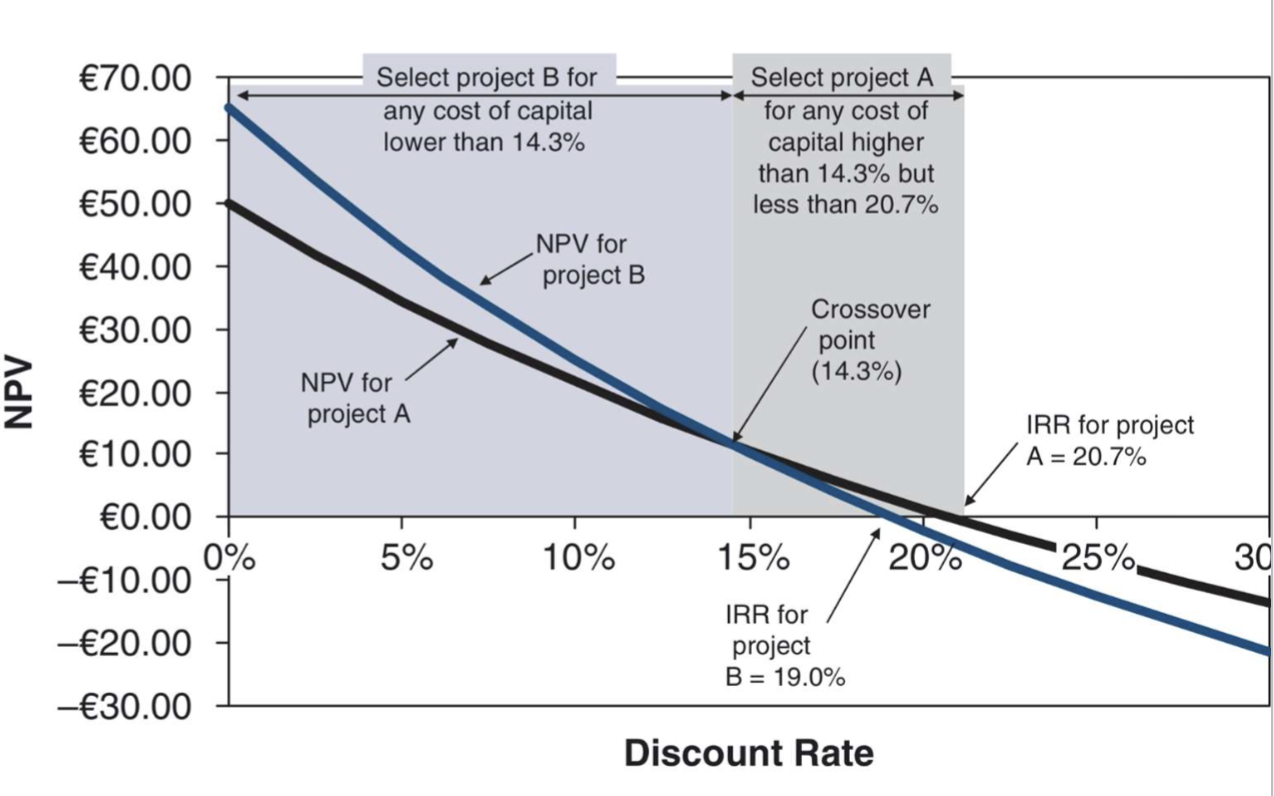
\includegraphics[scale=0.5]{1.png}
     \caption{Sammenhæng mellem $NPV$ og $IRR$}
     \label{Figur 2}
\end{figure} 

En anden begrænsning ved den interne rentefods metode er, at den antager, at indtægterne generet i løbet af perioden kan geninvesteres til den interne rente. Det følger af, at vi løser følgende ligning for at finde $IRR$; 

\begin{equation}
    IRR: \quad \sum_{t=0}^{n} \frac{C_t}{(1 + IRR)^t} = 0
\end{equation}

Det vil sige, hvad den den årlige indbetaling skal diskonteres med for at nettonutidsværdien er lig 0. Men det er jo det samme som at sige, $C_t$ hvert år vokser med $IRR$. Det er vist matematik nedenfor, hvor den samlede fremtidsværdi (FV) af alle pengestrømme, når de geninvesteres til $IRR$, er summen af fremtidsværdierne af alle individuelle pengestrømme:

\begin{equation*}
FV = \sum_{t=0}^{n} C_t \times (1 + IRR)^{n-t}
\end{equation*}

For at beregne NPV, diskonterer vi nu denne samlede fremtidsværdi (FV) tilbage til nutidsværdien ved brug af $IRR$:

\begin{equation*}
NPV = \frac{FV}{(1 + IRR)^n}
\end{equation*}

Substituerer vi udtrykket for FV i NPV-formlen:

\begin{equation*}
NPV = \frac{\sum_{t=0}^{n} C_t \times (1 + IRR)^{n-t}}{(1 + IRR)^n}
\end{equation*}

Dette kan forenkles til:

\begin{equation*}
NPV = \sum_{t=0}^{n} \frac{C_t \times (1 + IRR)^{n-t}}{(1 + IRR)^n}
\end{equation*}

Vi ser, at \( (1 + IRR)^{n-t} \) i tælleren og \( (1 + IRR)^n \) i nævneren kan kombineres til:

\begin{equation*}
NPV = \sum_{t=0}^{n} \frac{C_t}{(1 + IRR)^t}
\end{equation*}

Hvilket netop viser, at den interne rentefods metode implicit antager, at de løbende indbetalinger kan investeres til $IRR$. Dette overvurderer typisk en investerings rentabilitet, idet den den korrekte antagelse er, at de løbende indtægter kan geninvesteres til kapitalomkostningen, $r$, og $r<IRR$, hvis investeringen skal gennemføres. Fordele ved den interne rentefods metode er: 

\begin{itemize}
    \item Intuitiv fordi vi er vant til at tænke i afkast
    \item Er for det meste ækvivalent med den teoretisk korrekte kapitalværdimetode
    \item Kan beregnes uden kendskab til diskonteringsrenten
\end{itemize}

Mens ulemperne er: 

\begin{itemize}
    \item Giver ikke altid en unik anbefaling
    \item Kan give forkerte anbefalinger om valget mellem to investeringsprojekter
    \item Antager at frigjort cash kan geninvesteres til den interne rente \(\rightarrow\) rentabiliteten overvurderes hvis frigjort cash kun forrentes til den lavere kapitalomkostning
    \item Kan \textbf{ikke} bruges, hvis to projekter med forskellig investeringsbeløb sammelignes, idet IRR ikke tager udgangspunkt i investeringsbeløbets størrelse. Et projekt med høj IRR kan således have lav NPV, hvis investeringsbeløbet er småt og vice versa. 
\end{itemize}

\subsection{Modificeret intern rente}
Den modificerede interne rente tager hensyn til, at de løbende indtægter ikke kan investeres til den interne rente, men snarere til kapitalomkostningen og er defineret som: 

\begin{equation}
MIRR = \left( \frac{\sum_{t=1}^{n} C_{t1} (1 + r_g)^{n-t}}{\sum_{t=0}^{n} \frac{C_{t2}}{(1 + r_f)^t}} \right)^{\frac{1}{n}} - 1
\end{equation}

Hvor $r_g$ henviser til reinvesteringsraten (hvad de årlige indtægter forrentes med) og $r_f$ henviser til finansieringsraten (renteudgifter forbundet med finansieringen). Brøken i sig selv repræsenterer således forholdet mellem fremtidsværdien af positive pengestrømme ($C_{t1}$) og nutidsværdien af alle udgifter ($C_{t2}$) forbundet med projektet. Det hele er så opløftet i $\frac{1}{n}$ og fratrukket 1 for at bruges til at finde den gennemsnitlige årlige interne rente (MIRR) over \textit{n} perioder.

\vspace{10 pt}

Den interne rente (IRR) og den modificerede interne rente (MIRR) er sammenfaldende i følgende to tilfælde:

\begin{enumerate}
  \item \textbf{Geninvesteringsrenten er lig med IRR:}
  Når geninvesteringsrenten (\(r_g\)) er lig med IRR, vil alle mellemliggende pengestrømme, som antages at blive geninvesteret til IRR, gøre MIRR lig med IRR. Dette betyder, at:
  \[
  r_g = r_f = IRR
  \]
  
  \item \textbf{Ingen mellemliggende pengestrømme:}
  Hvis der ikke er nogen mellemliggende pengestrømme (dvs. ingen positive eller negative pengestrømme mellem start- og slutpunktet af projektet), vil både IRR og MIRR beregne afkastet baseret på de samme ind- og udstrømninger. Det gælder f.eks. for projekter med kun en enkelt initial investering efterfulgt af en enkel positiv pengestrøm ved projektets afslutning. 
\end{enumerate}


\subsection{Profitabilitetsindeks}
Profitabilitetsindekset er defineret som: 

\begin{equation}
    PI = \frac{\text{Nutidsværdi af fremtidige pengestrømme}}{\text{Initial investering}} = \frac{NPV}{I}
\end{equation}

Og beskriver således den skabte værdi per krone investeret. Hvis der f.eks. er blevet investeret 100 kr. og nutidsværdien af de fremtidige pengestrømme er lig 110, er indekset 1,1, svarende til, at hver investeret krone er blevet til 1,1 kr. 

\vspace{10 pt}
Profitabilitetsindekset \textbf{kan bruges} til at opstille et beslutningskriterium ækvivalent med kapitalværdimetoden for en enkelt investering, $PI>1$ betyder, at nutidsværdien af de fremtidige pengestrømme er større end den initiale investering, hvilket svarer til, at NPV er positiv. Altså er de to ækvivalente i dette tilfælde. 

\vspace{10 pt}
Profitabilitetsindekset kan \textbf{ikke bruges} til at opstille et beslutningskriterium ækvivalent med kapitalværdimetoden, hvis der er tale om to investeringer, der skal sammenligne og disse ikke har samme skala. En investering med $NPV=500$ og $I=50$ vil således blive valgt over $NPV=1000$, $I=500$, selvom den anden investering har den højeste nutidsværdi.

\subsection{Kapitalværdimetoden når genanskaffelse er mulig}
Når genanskaffelse altid er mulig, kan vi ikke længere benytte den klassisk kapitalværdimetode, hvor vi vælger den investering med højest $NPV$, hvis de to investeringer vi sammenligner ikke har samme løbetid. Det skyldes, at $NPV$ beregnes på baggrund af en tidsperiode (og denne ikke er ens for de to), og vi bliver nødt til at omdanne begge investeringer til perpetuiter. Det gøres ved: 
\begin{enumerate}
    \item At finde den årlige betaling som en betalingsrække skaber. 
    \item At finde nutidsværdien af en perpetuitet af en række med den fundne årlige betaling og en given diskonteringsrate.
\end{enumerate}

Antag f.eks. at vi har to investeringer, \textbf{A} og \textbf{B}, og disse har $NPV=100, n=5$ og $NPV=80, n=3$, diskonteringsrenten for begge projekter er $r=0,1$. Vi kan finde den årlige betaling som de to rækker skaber ved at benytte den tidligere funde formel: 

\begin{equation}
    C = \frac{PV \cdot r}{1 - (1 + r)^{-n}}
\end{equation}

Altså; 

\begin{align*}
    C_1 &= \frac{100 \cdot 0,1}{1 - (1 + 0,1)^{-5}} = 26,37 \\
    C_2 &= \frac{100 \cdot 0,1}{1 - (1 + 0,1)^{-5}} = 32,16
\end{align*}

Hvor NPV er: 

\begin{align*}
    NPV_1 &= \frac{26,37}{0,1} = 263,7 \quad [\text{kr.}] \\
    NPV_1 &= \frac{32,16}{0,1} = 321,6 \quad [\text{kr.}]
\end{align*}

Hvis genanskaffelse  ikke er mulig, bør \textbf{A} vælges, mens \textbf{B} bør vælges, hvis genanskaffelse er mulig.

\subsection{Optimal levetid}
En investerings optimale levetid er ikke altid identisk med den maksimale levetid, idet der kan være store reperationsomkostninger i slutningen af den maksimale levetid. Hvis genanskaffelse er ikke muligt, er den optimale levetid den levetid, der maksimerer nutidsværdien af en enkel investering, mens den optimale levetid — under antagelse af, at genanskaffelse altid er muligt — er den levetid, der maksimerer NPV af en uendelig række investeringer. Eksempel 4 gennemgår et beregningsteknisk eksempel heraf. 

\begin{tcolorbox}[breakable, colback=red!5!white, colframe=red!50!black, title= Eksempel 4: Beregning af optimal levetid for når genanskaffelse er hhv. muligt og ikke muligt]
Betragt en investering med en initial omkostning på 100, der herefter generer nettobetalinger på: 70 (år 1), 50 (år 2), 30 (år 3), 10 (år 4) og -10 (år 5). Kapitalomkostningen er 7 pct. Hvis genanskaffelse \textbf{ikke er muligt} beregnes den optimale levetid ved at beregne NPV for hhv. 1 år, 2 år, 3 år osv., hvorefter den højeste vælges, altså; 
\begin{align*}
NPV_{1 \text{ år}} &= \frac{70}{(1+0,07)^1} - 100 = -34,58 \\
NPV_{2 \text{ år}} &= \frac{70+50}{(1+0,07)^2} - 100 = 9,09 \\
NPV_{3 \text{ år}} &= \frac{70+50+30}{(1+0,07)^3} - 100 = 33,58 \\
NPV_{4 \text{ år}} &= \frac{70+50+30+10}{(1+0,07)^4} - 100 = 41,21 \\
NPV_{5 \text{ år}} &= \frac{70+50+30+10-10}{(1+0,07)^5} - 100 = 34,08 \\
\end{align*}

Under disse forudsætning vil den optimale levetid være 4 år. Hvis genanskaffelse derimod \textbf{altid er mulig}, skal vi beregne de årlige indbetalinger vha. formel 44 og herefter beregne nutidsværdien af den uendelig betalingsrække. Altså; 
\begin{align*}
C{1 \text{ år}}  &= \frac{-34,58 \cdot 0,07}{1-(1+0,07)^{-1}} = -36,38 \\
C{2 \text{ år}} &= \frac{9,09 \cdot 0,07}{1-(1+0,07)^{-2}} = 5,03 \\
C{3 \text{ år}} &= \frac{33,58  \cdot 0,07}{1-(1+0,07)^{-3}} = 12,80\\
C{4 \text{ år}} &= \frac{41,21  \cdot 0,07}{1-(1+0,07)^{-4}} = 12,17 \\
C{5 \text{ år}} &= \frac{34,08  \cdot 0,07}{1-(1+0,07)^{-5}} = 8,31 
\end{align*}

Hvor nutidsværdierne er: 
\begin{align*}
NPV_{1 \text{ år}}  &= \frac{-36,38}{0,07} = -519,71 \\
NPV_{2 \text{ år}}  &= \frac{5,03}{0,07} = 71,85 \\
NPV_{3 \text{ år}} &= \frac{12,8}{0,07} = 182,85 \\
NPV_{4 \text{ år}}  &= \frac{12,17}{0,07} = 173,85 \\
NPV_{5 \text{ år}}  &=  \frac{8,31}{0,07} = 118,71 
\end{align*}

I tilfælde af, at genanskaffelse er mulig, er den optimale levetid altså 3 år, modsat de fire år, som galt, hvor genanskaffelse ikke var mulig.
\end{tcolorbox}

\section{\textit{Opvarmning} til finansiering}
Finansieringsteori omhandler både virksomhedens passiv- og aktivside, alt afhængigt af, om virksomheden er lånegiver (debitor) eller lånetager (kreditor).  Der således en dobbelthed ved finansielle aktiver, der beskriver, at: 

\begin{itemize}
    \item Låntager får et passiv (skylder penge væk)
    \item Långiver får et aktiv (har penge til gode)
\end{itemize}

Denne dobbelthed eksisterer ikke ved anlægsinvesteringer, det gælder f.eks. ikke at en anden må \textit{skylde en bil}, hvis jeg ejer en bil. Når virksomheder eller personer investerer i værdipapirer eller obligation (dvs. får et aktiv), vil vi altid antage følgende: 

\begin{itemize}
    \item Investorer er \textbf{afkastsøgende}: hvis to værdipapirer har
samme risiko, foretrækkes det med højst forventet afkast
\item Investorer er \textbf{risikoaverse}: hvis to værdipapirer har samme
forventede afkast, foretrækkes det mindst risikofyldte. Det betyder dog ikke, at investorer ikke vil investere i risikofyldte aktier/obligationer, men blot, at de skal kompenseres for dette. 
\end{itemize}

De to antagelser er oftest i strid med hinanden og der opstår derfor et \textit{expected risk-return tradeoff}, hvor investoren skal \textit{vælge} mellem risiko og afkast (alt andet lige). 

\subsection{Nomenklatur for lån og obligationer}
I kurset beskæftiger vi os med følgende typer gæld: 

\begin{itemize}
    \item \textbf{Banklån}, herunder kassekredit (kortfristet) og erhvervslån (langfristet). 
    \item \textbf{Realkreditlån} $\rightarrow$ lån med pant i fast ejendom (langfristet).
    \item \textbf{Virksomhedsobligationer} $\rightarrow$ lån direkte fra investorer, ofte med hjælp fra investeringsbank (typisk langfristet).
    \item \textbf{Leverandørkredit} (kortfristet).
\end{itemize}

Hvor de følgende begreber bruges: 

\begin{itemize}
    \item \textbf{Hovedstol}: Det samlede beløb, der skal betales tilbage ifølge låneaftalen (ekskl. renter).
    \item \textbf{Kurs}: ``Prisen'' på lånet. (fx kurs 88 betyder, at der ved et lån på 100 kr. kun udbetales 88 kr.).
    \item \textbf{Kurstab}: Omkostning som følge af kurs $<$ 100 (i eksemplet ovenfor er der et kurstab på 12 kr.).
    \item \textbf{Andre omkostninger}: Fx stempelafgift/tinglysningsafgift (til staten), provision og gebyrer (til banken), bidrag (til realkreditinstituttet).
    \item \textbf{Provenu}: Det beløb man får udbetalt, når alle omkostninger til optagelse af lånet er afholdt.
    \item \textbf{Løbetid}: Lånets tilbagebetalingstid
    \item \textbf{Termin}: Tidspunkt for betaling på lånet (fx 4 årlige terminer).
    \item \textbf{Ydelse}: Det beløb, der betales til terminen. Består af renter og afdrag.
    \item \textbf{Afdrag}: Løbende tilbagebetaling af lånets hovedstol.
    \item \textbf{Amortisering}: Fancy ord for afdrag.
    \item \textbf{Restgæld}: Den del af lånets hovedstol, som ved et givent tidspunkt endnu ikke er betalt via de løbende afdrag.
\end{itemize}

Der er desuden følgende forskellige typer lån: 

\begin{itemize}
    \item \textbf{Kassekredit}
    \begin{itemize}
        \item Aftale om lån op til en øvre grænse, fleksibel afdragsprofil
        \item Der betales kun rente af det faktiske lån
        \item Der betales derudover ofte provision af det maksimale lån
    \end{itemize}
    
    \item \textbf{Stående lån}
    \begin{itemize}
        \item Der betales løbende renter til hver termin, men ingen afdrag
        \item Hele hovedstolen betales tilbage ved lånets udløb
    \end{itemize}

    \item \textbf{Annuitetslån}
    \begin{itemize}
        \item Samme konstante ydelse (rente + afdrag) hver termin indtil lånets udløb
        \item Rentebetalinger falder i løbet af lånets løbetid, afdrag stiger
    \end{itemize}

    \item \textbf{Serielån}
    \begin{itemize}
        \item Konstante afdrag hver termin indtil lånets udløb
        \item Renter og ydelse falder i løbet af lånets løbetid
    \end{itemize}
\end{itemize}

De forskellige afdragsprofiler er illustreret nedenfor: 

\begin{figure}[h]
     \centering
     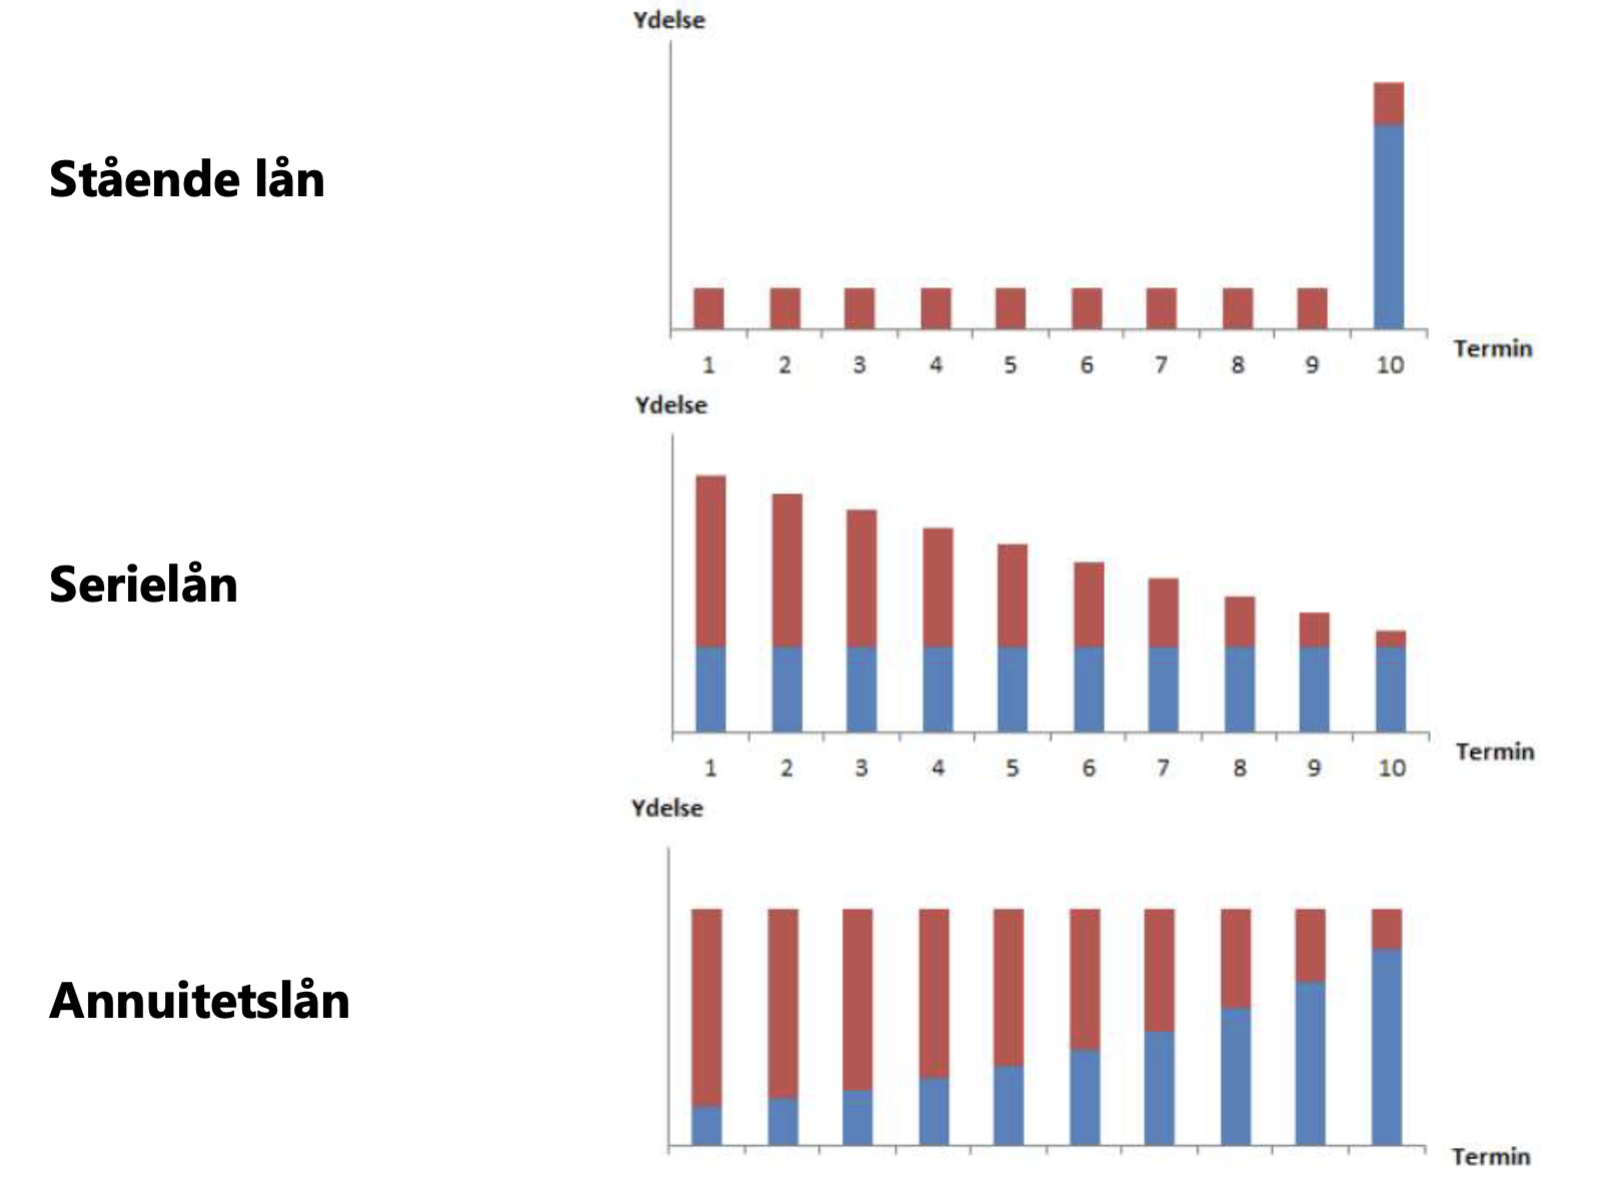
\includegraphics[scale=0.25]{5.png}
     \caption{Oversigt over forskellige afdragsprofiler}
     \label{Figur 2}
\end{figure} 

Ved annuitetslånet kan den årlige ydelse bestemmes ved hjælp af formel 35. Det bemærkes desuden, at ydelsen er konstant, men at rente/afdragsforholdet ændrer sig og nettoydelsen således stiger, idet renter kan trækkes fra i skat. 


\subsection{Forskellige rentebegreber}
\textbf{Den pålydende rente} (også kendt som nominel rente eller kuponrente) beskriver den årlige rente, der fremgår af låneaftalen. Denne rentetyper tager ikke højde for omkostninger forbundet med lånet, renters rente eller lign. og afspejler derfor (som regel) ikke de reelle omkostninger ved lånet. Hvis man f.eks. optager et lån, hvor den pålydende rente er 10 pct., men der er kvartalsvis rentetilskrivning (dvs. 2,5 pct. per kvartal), vil den faktiske årlige rente være givet ved: $(1+0,025)^4-1=10,3 \quad \text{pct.}$. Omregningen mellem kvartalsvise renter $r_t$ og årlige rente er generelt: 

\begin{equation}
    r_{\text{årlig}} = (1+r_t)^4 - 1
\end{equation}

\vspace{10 pt}

\textbf{Den effektive rente} ($ER$) er derimod det relevante mål for omkostningerne forbundet med et lån, og er defineret som den rente, der sikrer, at nutidsværdien af alle fremtidige betalinger er lig 0. Altså;  

\begin{equation}
    -PR + \sum_{t=1}^{T} Y_t (1 + ER)^{-t} = 0 \iff PR = \sum_{t=1}^{T} Y_t (1 + ER)^{-t}
\end{equation}

hvor $PR$ er lånets provenu, og $Y_t$ er lånets ydelse i periode $t$. Fordelen ved den effektive rente er, at den udtrykker de faktiske årlige omkostninger i forholdet til låneprovenuet og således er sammenligneligt på tværs af lån. I daglig tale kaldes den effektive rente også ÅOP (årlige omkostninger i procent). Selvom den effektive rente er et godt mål for en virksomheds omkostninger i forbindelse med at optage et lån, kan man ikke altid slutte at en lav $ERR$ er lig et attraktivt lån. Andre kriterier som de nedenstående er også relevante at have med i sin betragtning: 

\begin{itemize}
    \item Størrelsen af provenuet skal matche finansieringsbehovet. 
    \item Fleksibilitet — det fulde finansieringsbehov er ikke altid kendt på forhånd. 
    \item Ydelsesprofilen skal matche virksomhedens likviditetssituation. 
\end{itemize}

Eksempel 5 gennemgår to beregninger af den effektive rente. 

\begin{tcolorbox}[breakable, colback=red!5!white, colframe=red!50!black, title= Eksempel 5: Beregning af effektiv rente]
Betragt et lån på 50.000 kr. med en pålydende rente på 10 pct. p.a., der betales hvert kvartal ($50.000 \cdot 0,025 =1.250 kr.$) . Stiftelsesgebyret er 2.000 kr. og renterne betales i termin 1-19, hvorefter hovedstolen, samt renterne betales i periode 20. Den effektive kan da bestemmes som:  

\begin{equation*}
    48{.}000 = \left[ \sum_{t=1}^{19} 1{.}250 \cdot (1 + ER_T)^{-t} \right] + 51{.}250 \cdot (1 + ER_T)^{-20}
\end{equation*}

hvor $ER_T$ er den effektive rente per termin. Beregningen laves i Excel på baggrund af en amortationsplan og kommandoen $IRR$. Svaret bliver $ER_T$ = 0,0276 og $ER = (1+0,0276)^4 - 1 = 11,52$
\end{tcolorbox}

\subsection{Obligationer}
En obligation er en kontrakt, der giver køberen ret til at modtage en række fremtidige betalinger, beskrevet ved pålydende rente (kuponrenten), løbetid og afdragsprofil. Ved at sælge en obligation giver køberen altså et lån til sælgeren om de aftalte betalinger. Salgsprisen på en obligation kaldes kursen og fastsættes på markedet, hvor obligationer også kan sælges. En obligation indfries altid til kurs 100, hvorfor køber opnår en kursgevinst, hvis obligationen købes til $\text{kurs}<100$, mens køber opnår et kurstab, hvis $\text{kurs}>100$. 

\vspace{10 pt}

Kursen af en obligation bestemmes på baggrund af udbud og efterspørgsel. En given investor vil således være villig til at betale nutidsværdien af alle fremtidige betalinger som obligationen giver anledning til for en given obligation. Kalkulationsrenten sættes her til markedsrenten, idet det er det alternative afkast for investoren. En højere markedsrenten fører altså til en lavere obligationspris, idet de løbende udbetalinger diskonteres med en højere rente. Obligationskursen kan således være under 100, hvis \textbf{markedsrenten er højere end obligationsrenten}, mens den kan være over 100, hvis \textbf{markedsrenten er lavere end obligationsrenten}. Den kan også være lig 100, hvis \textbf{markedsrenten er lig obligationsrenten}. Intuitionen er, at når markedsrenten stiger, så forbedres afkastet på de alternative investeringer, hvilket svækker efterspørgslen efter obligationer, hvorfor prisen falder. I praksis vil den effektive rente via markedskræfterne bliver cirka lig markedsrenten. Det betyder dog ikke, at alle obligationer vil have samme effektive rente. Vi skal nemlig huske, at markedsrenten er lig med det alternative afkast man kan få ved samme risikoprofil og samme tidsperiode. Obligationer med forskellige tidsprofiler og forskellig risiko vil derfor have forskellig effektiv rente. Kortere løbetid og lavere risiko giver således ofte lavere effektiv rente, mens længere løbetid og højere risiko giver en højere effektiv rente. 

\vspace{10 pt}

Eksempel 6 gennemgår mekanikken bag en obligation og dens udbetalinger. 

\begin{tcolorbox}[breakable, colback=red!5!white, colframe=red!50!black, title= Eksempel 5: Obligationer og udbetalinger]
Betragt en obligation, der handles til kurs 90 med en pålydende rente på 2 pct. og en løbetid på 3 år, der afdrages som et stående lån med årlige terminer. Den effektive rente er nu lig den rente, der sikrer, at nutidsværdien af alle fremtide betalinger er lig 0, hvilket med omskrivning jf. formel 46 kan skrives som: 

\begin{equation}
    90 = 2 \cdot (1+ER)^{-1} + 2 \cdot (1+ER)^{-2} + 102 \cdot (1+ER)^{-3}
\end{equation}

Den effektive rente kan nu findes vha. solver i Excel og blev bestemt til 5,72 pct. Hvis kursen er lavere, vil den effektive rente stige. Kursen af obligationen er, som nævnt ovenfor, lig med nutidsværdien af alle fremtidige betalinger som obligationen giver anledning til. Ved en diskonteringsrente på hhv. 1 pct., 2 pct. og 3 pct. fås: 
\begin{align*}
    NPV_{r=1 \text{pct}} &= \frac{2}{(1+0,01)^1} + \frac{2}{(1+0,01)^2} + \frac{102}{(1+0,01)^3} = 102,94 \\
    NPV_{r=2 \text{pct}} &= \frac{2}{(1+0,02)^1} + \frac{2}{(1+0,02)^2} + \frac{102}{(1+0,02)^3} = 100 \\
    NPV_{r=2 \text{pct}} &= \frac{2}{(1+0,03)^1} + \frac{2}{(1+0,03)^2} + \frac{102}{(1+0,03)^3} = 97,17 
\end{align*}

Altså; at kursen falder, når diskonteringsrenten stiger. I vores tilfælde kan diskonteringsrenten findes vha. solver i Excel, og giver $r= 0,572$ pct. som netop er sammenfaldende med den effektive rente, idet markedsrente, der bruges til diskontering, også den effektive rente, som investoren forventer at modtage.
\end{tcolorbox}

\subsection{Måling af afkast}
\textbf{Afkastet ('total return')} i en enkelt periode $t$ er givet ved det cash flow værdipapireret har udbetalt og forskellen mellem købs- og salgsprisen. Altså;  

\begin{equation}
    TR_t = \frac{CF_t + (P_E - P_B)}{P_B}
\end{equation}

Hvor $CF_t$ beskriver cash flowet generet i perioden, $P_B$ beskriver prisen til starttidspunktet (primo) og $P_E$ beskriver prisen til sluttidspunktet (ultimo).

\vspace{10 pt}

\textbf{ Det relative afkast ('relative return')} er på tilsvarende vis defineret som: 

\begin{equation}
    RR_t = \frac{CF_t + P_E}{P_B}
\end{equation}

Hvor det gælder, at: 

\begin{equation}
    RR_t = TR_t + 1
\end{equation}

Hvis en aktie købes til 100, sælges til 110 og der i perioden modtages et udbytte på 15 kr. vil begge mål således give et afkast på 15 pct, som vist nedenfor: 
\begin{align*}
    TR_t &= \frac{5 + 10}{100} = 0,15 \\
    RR_t &= \frac{5 + 110}{100} = 1,15
\end{align*}

\vspace{10 pt}

\textbf{Det kumulative afkast} måler det samlede afkast over flere perioder og er defineret som produktet af de relative afkast. Altså; 

\begin{equation}
    CR_n = RR_1 \cdot RR_2 \cdot \dots RR_n
\end{equation}

Dette afkast aflæses på samme måde som det relative afkast, dvs. et kumulative afkast på \textit{X}-pct betyder, at det samlede afkast over \textit{n} perioder har været \textit{X}-pct. Det kumulative afkast fås kun approksimativt ved at lægge $TR$ samme for hver periode. 

\vspace{10 pt}

Hvis man ønsker at beskrive, hvad det bedste bud på afkastet er i et tilfældigt år, skal vi benytte os af det \textbf{aritmetiske gennemsnit} af $TR$. Altså; 

\begin{equation}
    \overline{TR} = \frac{1}{n} \sum_{i=1}^{n} TR_i = \frac{1}{n} (TR_1 + TR_2 + TR_3 + \ldots + TR_n)
\end{equation}

Det gælder, da det aritmetiske gennemsnit ikke tager højde for nogen renters-rente effekt (da det blot er gennemsnittet af $TR$), og således er det bedste estimat for afkastet i et tilfældigt år. 

\vspace{10 pt}

Hvis man derimod ønsker at estimere, hvad det gennemsnitlige årlige afkast af at holde en aktie over en given periode, er det \textbf{geometriske gennemsnit} bedre at bruge, idet dette netop tager højde for renters-rente effekten. Det geometriske gennemsnit er defineret som: 

\begin{equation}
    G = \left( \prod_{i=1}^{n} RR_i \right)^{\frac{1}{n}} - 1
\end{equation}

Det gælder generelt, at jo større forskel der er mellem de enkelte års afkast, jo større vil forskellen mellem det aritmetiske og geometriske gennemsnit være. De to er kun lig hinanden, hvis det årlige afkast er konstant i hver periode. Ellers vil det aritmetiske gennemsnit altid være større end det geometriske. Det skyldes, at det geometriske gennemsnit i højere grad bliver påvirket af ekstremer end det aritmetiske gennemsnit. Det skyldes, at produktet af tal med stor variation (store udsving) har en tendens til at trække gennemsnittet ned. Det gælder derfor altid, at: 

\begin{equation}
\frac{TR_1 + TR_2 + \ldots + TR_n}{n} \geq \sqrt[n]{(TR_1+1) \cdot (TR_2+1) \cdot \ldots \cdot (TR_n+1)}
\end{equation}

\section{Porteføljeteori}
\subsection{Antagelser i porteføljeteori og diversifikationsprincippet}
I porteføljeteori gør vi følgende antagelser: 

\begin{itemize}
    \item Investoren kan investere i et endeligt antal forskellige
værdipapirer. 
\item Kan placere en hvilket som helst andel af formuen i hvert
værdipapir, ingen transaktionsomkostninger.
\item Fundamental usikkerhed omkring værdipapirernes
fremtidige afkast.
\item Samt de kendte antagelser om risikoaversion og afkastsøgende investorer.
\end{itemize}

Det gælder desuden, at: \textit{portføljerisikoen for en portefølje bestående af forskellige værdipapirer er mindre end eller lig det
vægtede gennemsnit af risikoen for de enkelte værdipapirer i porteføljen}. Heraf følger det, at man kan minimere sin porteføljerisiko ved at vælge de \textit{rigtige} værdipapirer, så summen af disse mindsker den samlede risiko (varians). Det følger heraf at; (1) den samlede risiko kan mindskes uden at afkastet bliver mindre (hvis to værdipapirer tilsammen giver lavere risiko, men hver især har det afkast). Desuden (2) gælder det, at den samlede risiko reduceres lidt, hvis der tilføjes en aktie, der i høj grad samvarierer med porteføljen, mens risiko reduceres meget (3), hvis der tilføjes en aktie, der i lav grad samvarierer med porteføljen. 

\vspace{10 pt}

Diversifikationsprincippet tilsiger således, at man ved tilstrækkelig diversifikation kan fjerne den idiosynkratiske (virksomhedsspecifikke) risiko, f.eks. om Volskwagen igen snyder med deres udledninger, mens man ikke kan fjerne den systematiske, markedsrelaterede risiko, f.eks. sandsynligheden for at jorden rammes af en komet eller der pludselig kommer en stor recession i EU. I porteføljeteori forsøger vi at lave historiske analyser af aktier for at bestemme, hvilke aktier, der kan reducere risikoen i vores portefølje og/eller øge det samlede afkast. Til dette bruger vi følgende statistiske værktøjer, der introduceres i det følgende afsnit: 

\begin{itemize}
    \item Værdipapirernes gennemsnitlige afkast $\rightarrow$ aritmetisk gennemsnit af $TR$
    \item Estimat for risiko $\rightarrow$ varians
    \item Graden af samvariation mellem afkastene $\rightarrow$ kovarians
\end{itemize}

Vi antager dermed implicit, at sandsynlighedsfordelingerne for afkast i
fremtiden vil være omtrent, som de har været i fortiden. 

\subsection{Introduktion til stokastiske variable}
De følgende værktøjer tager udgangspunkt i \textbf{Stokastiske variable}, dvs. en variabel, $X$, hvis værdi er usikker på forhånd. Det gælder dog, at de $I$ mulige udfald er kendte (udfaldsrummet) og der til dem er knyttet værdier af $X$; $x_1, x_2, \ldots, x_n$ (værdisættet). Desuden er der en sandsynlighed, $p_1, p_2, \ldots, p_n$ tilknyttet hver udfald (sandsynlighedsfordelingen over udfaldsrummet). Den realiserende værdi er den faktiske værdi, $x$, som $X$ antager efter \textit{usikkerheden udløses}. Det gælder desuden, at en sandsynlighedsfordeling er diskret, hvis der er et endeligt antal udfald. I dette tilfælde vil sandsynlighederne summe til 1. Et eksempel herpå er et terningekast af en 6-siddet terning, hvor $x=1,2,3,4,5,6$, og $p=\frac{1}{6}$. 

\vspace{10 pt}

Hvis vi antager, at det fremtidige afkast af et værdipapir er givet ved en stokastisk variabel, og vi kender sandsynlighedsfordelingen, kan \textbf{middelværdien} eller \textbf{den forventede værdi} bestemmes ved det vægtede gennemsnit af udfaldende og deres sandsynligheder over hele udfaldsrummet. Altså; 

\begin{equation}
    E(X) = \sum_{i=1}^{I} p_i x_i
\end{equation}

Fortolkningen heraf er, at det er den gennemsnitlig værdi, der opnås, hvis $X$ realiseres \textit{mange gange}. 

\vspace{10 pt}

For at beregne risikoen af en aktie, udtrykker vi risiko som omfanget af
variabilitet, dvs. hvor meget afkastet typisk varierer omkring gennemsnittet. Som mål for dette benyttes \textbf{variansen}, der for en diskret sandsynlighedsfordeling er givet ved middelværdien af den kvadrede afvigelse fra den forventede værdi. Årsagen til, at afvigelsen kvadreres er, at positive og negative afvigelser skal \textit{behandles} ens matematisk. 

\begin{equation}
    \sigma_X^2 = E \left( [X - E(X)]^2 \right) = \sum_{i=1}^{I} \left[ x_i - E(X) \right]^2 p_i
\end{equation}

En lille varians betyder her, at de mulige værdier ligger tæt på den forventede værdi (og værdier langt fra den forventede værdi er usandsynlige), mens en stor varians betyder, at de mulige værdier ligger langt fra den forventede værdi (og værdier tæt på den forventede værdi er usandsynlige). 

\vspace{10 pt}

\textbf{Standardafvigelsen} er blot kvadratroden af variansen og benyttes fordi den nu er i samme enhed som den pågældende variabel og dermed er lettere at fortolke. Altså; 

\begin{equation}
    \sigma_X = \left( \sum_{i=1}^{I} \left[ x_i - E(X) \right]^2 p_i \right)^{\frac{1}{2}} = \sqrt{\sigma_X^2}
\end{equation}

\newpage
\textbf{Kovariansen} mellem to stokastiske variable er estimat for samvariationen mellem de to variable, og er defineret som middelværdien af de to variables afvigelser fra deres middelværdi. Definitionen er da: 

\begin{equation}
    \sigma_{XY} = E\left( [X_i - E(X)][Y_i - E(Y)] \right) = \sum_{i=1}^{I} \left[ x_i - E(X) \right] \left[ y_i - E(Y) \right] p_i
\end{equation}

Udfordringen ved kovariansmålet er dog, at det afhænger af de stokastiske variables størrelse. Betragt f.eks. to variable, der med 50 pct. sandsynlighed tager værdien 1 og med 50 pct. sandsynlighed tager værdien 0. Kovariansen bliver her: 

\begin{equation*}
    \sigma_{XY} = [(1-0,5)][(1-0,5)]\cdot \frac{1}{2} + [(0-0,5)][(0-0,5)]\cdot \frac{1}{2} = 0,25 
\end{equation*}

Mens kovariansen stiger, når variablene pludselig tiltager værdien 100 med 50 pct. sandsynlighed og 0 med 50 pct. sandsynlighed: 

\begin{equation*}
    \sigma_{XY} = [(100-50)][(100-50)]\cdot \frac{1}{2} + [(0-50)][(0-50)]\cdot \frac{1}{2} = 2500
\end{equation*}

Det udledes nedenfor, hvad kovariansen bliver, når $\sigma_x = \sigma_y$,  $\sigma_x = -\sigma_y$, samt når variablene er ukorrelerede.
\begin{tcolorbox}[breakable, colback=red!5!white, colframe=red!50!black, title= Udledning af sammenhænge indenfor kovarians]

Hvis $x_i = y_i$ i alle udfald, vil $\sigma_{XY} = \sigma_X^2 = \sigma_Y^2$. Det kan nemt ses ved at indsætte $x_i = y_i$ i udtryk 58 og simplificere: 
\begin{equation*}
\sigma_{XY} = E\left( [X - E(X)]^2 \right)
\end{equation*}
Da $[X - E(X)]^2$ er variansen af $X$:
\begin{equation*}
\sigma_{XY} = \sigma_X^2
\end{equation*}
Og da $x_i = y_i$, har vi også, at $\sigma_X^2 = \sigma_Y^2$. Derfor er:
\begin{equation*}
\sigma_{XY} = \sigma_X^2 = \sigma_Y^2
\end{equation*}

På tilsvarende vis vil det gælde, at  at $\sigma_{XY} = -\sigma_X^2 = -\sigma_Y^2$, hvis $x_i = -y_1$. Det følger ved indsættelse, at: 

\begin{equation*}
\sigma_{XY} = E\left( [X - E(X)][-X - E(Y)] \right)
\end{equation*}
Vi ved, at $E(Y) = E(-X) = -E(X)$, så vi kan skrive:
\begin{equation*}
\sigma_{XY} = E\left( [X - E(X)][-X - (-E(X))] \right)
\end{equation*}
Dette forenkler til:
\begin{equation*}
\sigma_{XY} = E\left( [X - E(X)][-X + E(X)] \right)
\end{equation*}
Vi kan nu faktorisere udtrykket:
\begin{equation*}
\sigma_{XY} = E\left( [X - E(X)] \cdot [-1 \cdot (X - E(X))] \right)
\end{equation*}
Dette giver os:
\begin{equation*}
\sigma_{XY} = E\left( -[X - E(X)]^2 \right)
\end{equation*}
Da den forventede værdi af et produkt af en konstant og en variabel er lig med konstanten gange forventningen af variablen, kan vi tage konstanten -1 udenfor den forventede værdi:
\begin{equation*}
\sigma_{XY} = -E\left( [X - E(X)]^2 \right)
\end{equation*}
Da $[X - E(X)]^2$ er variansen af $X$:
\begin{equation*}
E\left( [X - E(X)]^2 \right) = \sigma_X^2
\end{equation*}
Så kan vi konkludere, at:
\begin{equation*}
\sigma_{XY} = -\sigma_X^2
\end{equation*}
Og da $\sigma_X^2 = \sigma_Y^2$:
\begin{equation*}
\sigma_{XY} = -\sigma_Y^2
\end{equation*}

Afsluttende vil det gælde, at to uafhængige variable vil have $\sigma_{XY} = 0$. Da det for uafhængige variable gælder, at:
\begin{align*}
\sigma_{XY} &= E\left( [X - E(X)][Y - E(Y)] \right) \\
&= E\left( XY - XE(Y) - E(X)Y + E(X)E(Y) \right) \\
&= E(XY) - E(XE(Y)) - E(E(X)Y) + E(E(X)E(Y)) \\
&= E(XY) - E(X)E(Y) - E(X)E(Y) + E(X)E(Y) \quad (\text{omskrivning pga. linearitet}) \\
&= E(XY) - E(X)E(Y) \\
&= E(X)E(Y) - E(X)E(Y) \quad (\text{da } X \text{ og } Y \text{ er uafhængige}) \\
&= 0
\end{align*}
\end{tcolorbox}

For at \textit{fjerne} de stokastiske variables indflydelse på kovariansen introduceres begrebet \textbf{korrelationskoefficient}, der er defineret som: 

\begin{equation}
    \rho_{XY} = \frac{\sigma_{XY}}{\sigma_X \cdot \sigma_Y}
\end{equation}

Som altså udtrykket samvariation nøjagtigt som kovariansen, men er skaleret i intervallet $[-1,1]$, hvor $-1$ svarer til negativ 1:1 korrelation, $0$ svarer til ingen korrelation og $1$ svarer til en positiv 1:1 korrelation. I tilfældet ovenfor bliver korrelationskoefficienten for de stokastiske variable med 50 pct. sandsynlighed antager værdien 1 og 50 pct. antager værdien 0: 

\begin{equation*}
  \rho_{XY} = \frac{0,25}{\sqrt{[((1-0,5)^2 + (0-0,5)^2) \cdot \frac{1}{2}]} \cdot \sqrt{[((1-0,5)^2 + (0-0,5)^2) \cdot \frac{1}{2}]}} = \frac{0,25}{\sqrt{0,25} \cdot \sqrt{0,25}} = \frac{0,25}{0,25} = 1
\end{equation*}

Og i tilfælde af, at de har samme sandsynlighedsfordeling, men tiltager værdierne 0 og 100: 

\begin{equation*}
    \rho_{XY} = \frac{2500}{\sqrt{[((100-50)^2 + (0-50)^2) \cdot \frac{1}{2}]} \cdot \sqrt{[((100-50)^2 + (0-50)^2) \cdot \frac{1}{2}]}} = \frac{2500}{\sqrt{2500} \cdot \sqrt{2500}} = \frac{2500}{50 \cdot 50} = 1
\end{equation*}

I eksempel 6 gennemgås beregningen af såvel varians og korrelationskoefficient. 

\begin{tcolorbox}[breakable, colback=red!5!white, colframe=red!50!black, title= Eksempel 6: Beregning af varians og korrelationskoefficient]
\textbf{1. Bestem variansen af den stokastiske variabel, $X$, der måler antallet af prikker ved et enkelt terningekast: }
\[
E[X] = \sum_{i=1}^{6} p_i x_i = \frac{1}{6} \cdot 1 + \frac{1}{6} \cdot 2 + \frac{1}{6} \cdot 3 + \frac{1}{6} \cdot 4 + \frac{1}{6} \cdot 5 + \frac{1}{6} \cdot 6 = 3.5
\]

\[
\sigma_X^2 = \sum_{i=1}^{6} (x_i - E[X])^2 p_i = (1 - 3.5)^2 \cdot \frac{1}{6} + (2 - 3.5)^2 + \ldots + (6 - 3.5)^2 \cdot \frac{1}{6} = 2.92
\]

\textbf{2. Hvad er kovariansen mellem for de to stokastiske variable, der er givet ved udfaldene af de to kast?}

\vspace{10 pt}

Lad \( X \) og \( Y \) være de stokastiske variable, der repræsenterer udfaldene af de to kast, hvor plat (0) og krone (1) er lige sandsynlige.

\[
\sigma_{XY} = \sum_{i=1,2,3,4} (x_i - E[X])(y_i - E[Y])p_i
\]

\[
E[X] = E[Y] = 0 \cdot \frac{1}{2} + 1 \cdot \frac{1}{2} = \frac{1}{2}
\]

\[
= \left( 0 - \frac{1}{2} \right) \cdot \left( 0 - \frac{1}{2} \right) \cdot \frac{1}{4} + \left( 0 - \frac{1}{2} \right) \cdot \left( 1 - \frac{1}{2} \right) \cdot \frac{1}{4} + \left( 1 - \frac{1}{2} \right) \cdot \left( 0 - \frac{1}{2} \right) \cdot \frac{1}{4} + \left( 1 - \frac{1}{2} \right) \cdot \left( 1 - \frac{1}{2} \right) \cdot \frac{1}{4}
\]

\[
= \left( -\frac{1}{2} \right) \cdot \left( -\frac{1}{2} \right) \cdot \frac{1}{4} + \left( -\frac{1}{2} \right) \cdot \left( \frac{1}{2} \right) \cdot \frac{1}{4} + \left( \frac{1}{2} \right) \cdot \left( -\frac{1}{2} \right) \cdot \frac{1}{4} + \left( \frac{1}{2} \right) \cdot \left( \frac{1}{2} \right) \cdot \frac{1}{4} = 0
\]
\end{tcolorbox}

\subsection{Regneregler for sammensatte stokastiske variable}
Betragt en stokastisk variabel $Z$, der er givet ved den vægtede sum af to andre stokastiske variable, altså; 

\begin{equation}
    Z = w_X \cdot X + w_Y \cdot Y
\end{equation}

hvor $w_X$ er vægten knyttet til $X$ og $w_Y$ er vægten knyttet til $Y$. \textbf{Middelværdien} af den sammensatte stokastiske variabel er nu blot den vægtede sum af middelværdien af de to komponenter, $X$ og $Y$. Altså; 

\begin{equation}
    E[Z] = w_X E[X] + w_Y E[Y]
\end{equation}

\textbf{Variansen} af $Z$ afhænger derimod både af de indbyrdes varianser, $X$ og $Y$, men samtidig også positivt af deres kovarians! Det følger af nedenstående: 

\begin{equation}
\sigma_Z^2 = w_X^2 \sigma_X^2 + w_Y^2 \sigma_Y^2 + 2 w_X w_Y \sigma_{XY}
\end{equation}

Altså; jo lavere kovarians mellem to aktier, jo lavere er den samlede varians for porteføljen $Z$ bestående af de to aktier, $X$ og $Y$. Vi kan omskrive formel 62 ved at indsætte $\sigma_{XY}= \rho_{XY} \cdot \sigma_X \cdot \sigma_Y$ (følger af formel 59). Udtrykket bliver så til: 

\begin{equation}
\sigma_Z^2 = w_X^2 \sigma_X^2 + w_Y^2 \sigma_Y^2 + 2 w_X w_Y \rho_{XY} \sigma_X \sigma_Y
\end{equation}

Altså; jo større korrelation mellem $X$ og $Y$, jo større varians har $Z$. Hvis korrelationskoefficenten er lig 1, bliver formel 63 til: 
\begin{align*}
    \sigma_Z^2 &= w_X^2 \sigma_X^2 + w_Y^2 \sigma_Y^2 + 2 w_X w_Y \sigma_X \sigma_Y \\
    \sigma_Z^2 &= (W_X \sigma_X + W_Y \sigma_Y)^2 \\
    \sigma_Z &= W_X \sigma_X + W_Y \sigma_Y
\end{align*}

Altså er variansen er $Z$ lig med den vægtede sum af standardafvigelsen af $X$ og $Z$, hvis $\rho_{XY}=1$. Tilsvarende følger det, at $\sigma_Z<W_X \sigma_X + W_Y \sigma_Y$, hvis $\rho_{XY}<1$. Generelt gælder det således, at:

\begin{equation}
    \sigma_Z \leq w_X \sigma_X + w_Y \sigma_Y + \ldots + w_n \cdot \sigma_n
\end{equation}

Som netop formaliserer vores indsigt om diversifikation, idet man ved at sammensætte en portefølje af flere værdipapirer med samme forventede
afkast, kan reducere risikoen, uden at det forventede afkast bliver lavere. Intuitionen er, at den højde risiko kun indgår 1 gang i form af variansen ganget med vægten, men at den lave korrelationskoefficient med de øvrige aktier indgår flere gange (den nye aktie korrellerer nemlig med flere aktier). I praksis gælder det, at \textbf{man ved at tilføje en aktie til en portefølje med $n$ elementer tilføjer 1 yderligere variansled og 2$n$ yderligere kovariansled}.

\vspace{10 pt}

Hvis korrelationskoefficienten er lig 0, bliver ligning 63 til: 
\begin{align*}
    \sigma_Z^2 &= w_X^2 \sigma_X^2 + w_Y^2\sigma_Y^2  \\
    \sigma_Z &= \sqrt{(w_X^2 \sigma_X^2 + w_Y^2\sigma_Y^2 )}
\end{align*}

\subsection{Stokastiske variable for empiriske stikprøver}
I virkelighedens verden kender vi ikke de teoretiske
populationsparametre (som vi er interesseret i), hvorfor vi i stedet estimerer dem på baggrund af stikprøver (f.eks. udsnit af afkastet for en aktie). Denne metode giver et godt estimat, hvis stikprøven er tilfældigt udtrukket. 

\vspace{10 pt}

\textbf{Det aritmetiske gennemsnit} for en stikprøve med $n$ realiserede afkast er er stikprøveækvivalenten til middelværdien og er defineret som: 

\begin{equation}
    \overline{X} = \frac{1}{n} \sum_{i=1}^{n} X_i
\end{equation}

\vspace{10 pt}

\textbf{Den empiriske varians} benyttes i stedet for den teoretiske varians, hvor der nu divideres med $n-1$ fremfor $n$ (Bessels korrektion). Altså;

\begin{equation}
    \hat{\sigma}^2 = \frac{\sum_{i=1}^{n} (X_i - \overline{X})^2}{n - 1}
\end{equation}

\textbf{Den empiriske standardafvigelse} er givet ved kvadratroden af den empiriske varians, altså; 

\begin{equation}
   \hat{\sigma}^2 = \hat{\sigma}
\end{equation}

\textbf{Den empiriske kovarians} er defineret som, hvor der nu divideres med $n-1$ fremfor $n$ (Bessels korrektion). 

\begin{equation}
    \hat{\sigma}_{XY} = \frac{1}{n - 1} \sum_{i=1}^{n} (X_i - \overline{X})(Y_i - \overline{Y})
\end{equation}

\textbf{Den empiriske korrelationskoefficient} er afslutningsvist givet ved: 

\begin{equation}
    \hat{\rho}_{XY} = \frac{\hat{\sigma}_{XY}}{\hat{\sigma}_X \cdot \hat{\sigma}_Y}
\end{equation}

Excel formlerne til beregning af ovenstående er vist nedenfor, og skal ALTID bruges, når der er tale om udsnit af data fra den \textit{virkelige verden}: 

\begin{figure}[h]
     \centering
     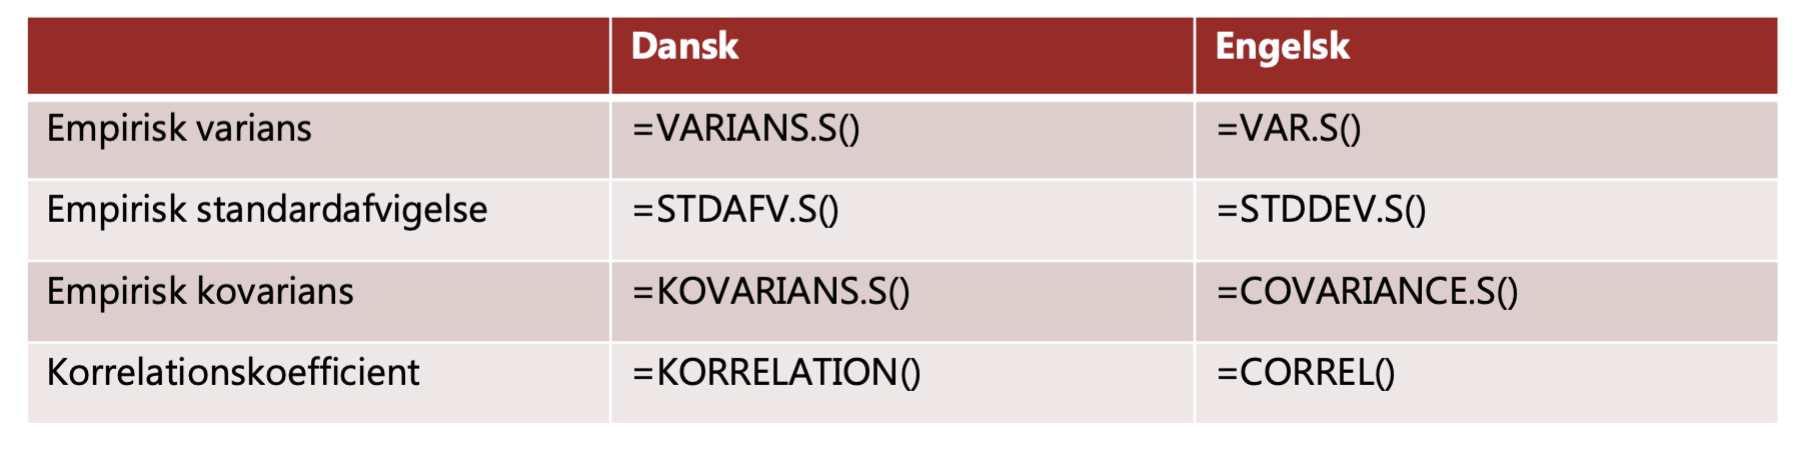
\includegraphics[scale=0.40]{6.png}
     \caption{Oversigt Excel kommandoer til beregning af empiriske stikprøver}
     \label{Figur 2}
\end{figure} 

\subsection{Anvendelse af stokastiske variable i porteføljesammenhænge}
Betragt en portefølje, $Z$, hvor afkastene af de enkelte aktier er udtrykt ved $R_1, R_2, \ldots, R_N$ med tilhørende vægte $w_1, w_2,\ldots, w_N$. Afkastet for porteføljen er da: 

\begin{equation}
    Z = w_1 \cdot R_1 + w_2 \cdot R_2 + \ldots + w_N \cdot R_N
\end{equation}

Hvor variansen af det samlede afkast kan skrives som: 

\begin{equation}
    \sigma_p^2 = \sum_i w_i^2 \sigma_i^2 + \sum_i \sum_{j \neq i} w_i w_j \sigma_{ij}
\end{equation}

hvor det, som bekendt, fremgår, at porteføljevariansen afhænger  af variansen af hver enkelt værdipapir i porteføljen samt af kovarianserne mellem værdipapirerne. I praksis gennemføres denne beregning nemmest vha. kovariansmatricer og en hjælpematrice, som illustreret i eksempel 7 nedenfor: 


\begin{tcolorbox}[breakable, colback=red!5!white, colframe=red!50!black, title= Eksempel 7: Beregning af varians for en sammensat portefølje vha. kovarians- og hjælpematricer]

Betragt en situation, hvor der er givet afkastsdata (målt ved TR) for 3 forskellige aktier, $A$, $B$ og $C$. Deres indiviudelle varians, samt kovariansne kan nu estimeres vha. kommandoer i Excel. På baggrund af et fiktivt datasæt fås: 
\begin{align*}
    \sigma_A^2 &= 0,07 \\
    \sigma_B^2 &= 0,25 \\
    \sigma_C^2 &= 0,79 \\
    \sigma_{AB} &= 0,06 \\
    \sigma_{AC} &= -0,09 \\
    \sigma_{BC} &= 0,2 
\end{align*}

For at bestemme variansen for den samlede porteføljen opstilles kovariansmatricen, der er defineret som: 

\begin{equation}
var(A,B,C, \ldots, n) = 
\begin{pmatrix}
\sigma_{AA} & \sigma_{AB} & \sigma_{AC} & \cdots & \sigma_{An} \\
\sigma_{BA} & \sigma_{BB} & \sigma_{BC} & \cdots & \sigma_{Bn} \\
\sigma_{CA} & \sigma_{CB} & \sigma_{CC} & \cdots & \sigma_{Cn} \\
\vdots & \vdots & \vdots & \ddots & \vdots \\
\sigma_{nA} & \sigma_{nB} & \sigma_{nC} & \cdots & \sigma_{nn}
\end{pmatrix}
\end{equation}

Med værdierne ovenfor bliver det til: 

\begin{equation*}
    var(A,B,C) =
\begin{pmatrix}
\sigma_A^2 & \sigma_{AB} & \sigma_{AC} \\
\sigma_{AB} & \sigma_B^2 & \sigma_{BC} \\
\sigma_{AC} & \sigma_{BC} & \sigma_C^2 \\
\end{pmatrix}
=
\begin{pmatrix}
0.07 & 0.06 & -0.09 \\
0.06 & 0.25 & 0.2 \\
-0.09 & 0.2 & 0.79 \\
\end{pmatrix}
\end{equation*}

For at beregne den endelige varians for porteføljen skal man nu opstille en hjælpematrice, der er lig kovariansmatricen ganget med aktiernes respektive vægte. Den samlede varians er så summen af hver række. Se nedenstående: 

\vspace{10 pt}
\begin{center}
        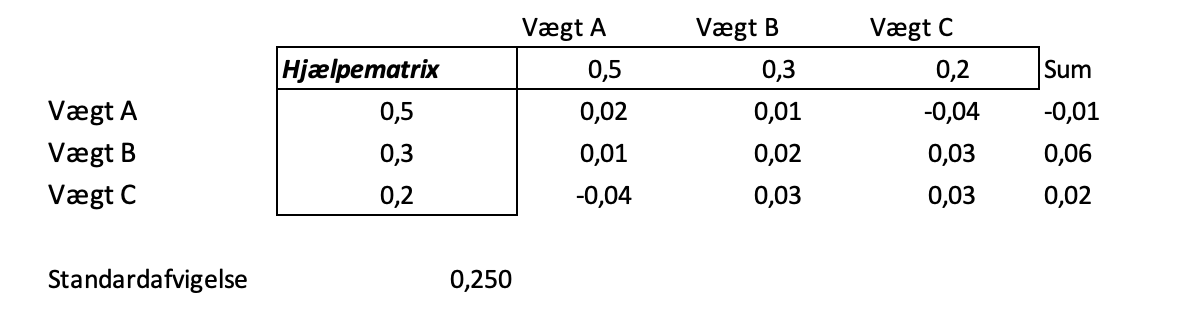
\includegraphics[width=0.8\textwidth]{8.png}
\end{center}

Hvor vægtene på aktierne er hhv. $A=0,5, B=0,3, C =0,2$. Standardafvigelsen bestemmes på kvadratrodden af de samlede summer, mens variansen blot er summen af summerne på rækkeled. Den samlede porteføljevarians er altså ca. $0,25^2 = 0,0625$, mens standardafvigelsen er 0,250. 
\end{tcolorbox}

\subsection{Den formelle porteføljeteori}
Den formelle porteføljeteori beskæftiger sig med spørgsmålet om, hvilken portefølje, $P$, en given investor skal vælge. Man antager i den forbindelse, at enhver kombination af $w_1, w_2, \ldots, w_n$ med $w_1, w_2, \ldots, w_n = 1$ er mulig, hvor $w$ angiver vægten af en given aktie. For hver portefølje kan med vha. de matematiske forudsætninger beskrevet i \textbf{5.4} beregne standardafvigelsen, $\sigma_P$, samt det forventede afkast: $E[R_p]$. Figuren nedenfor viser sammenhængen mellem de størrelser: 

\begin{figure}[h]
     \centering
     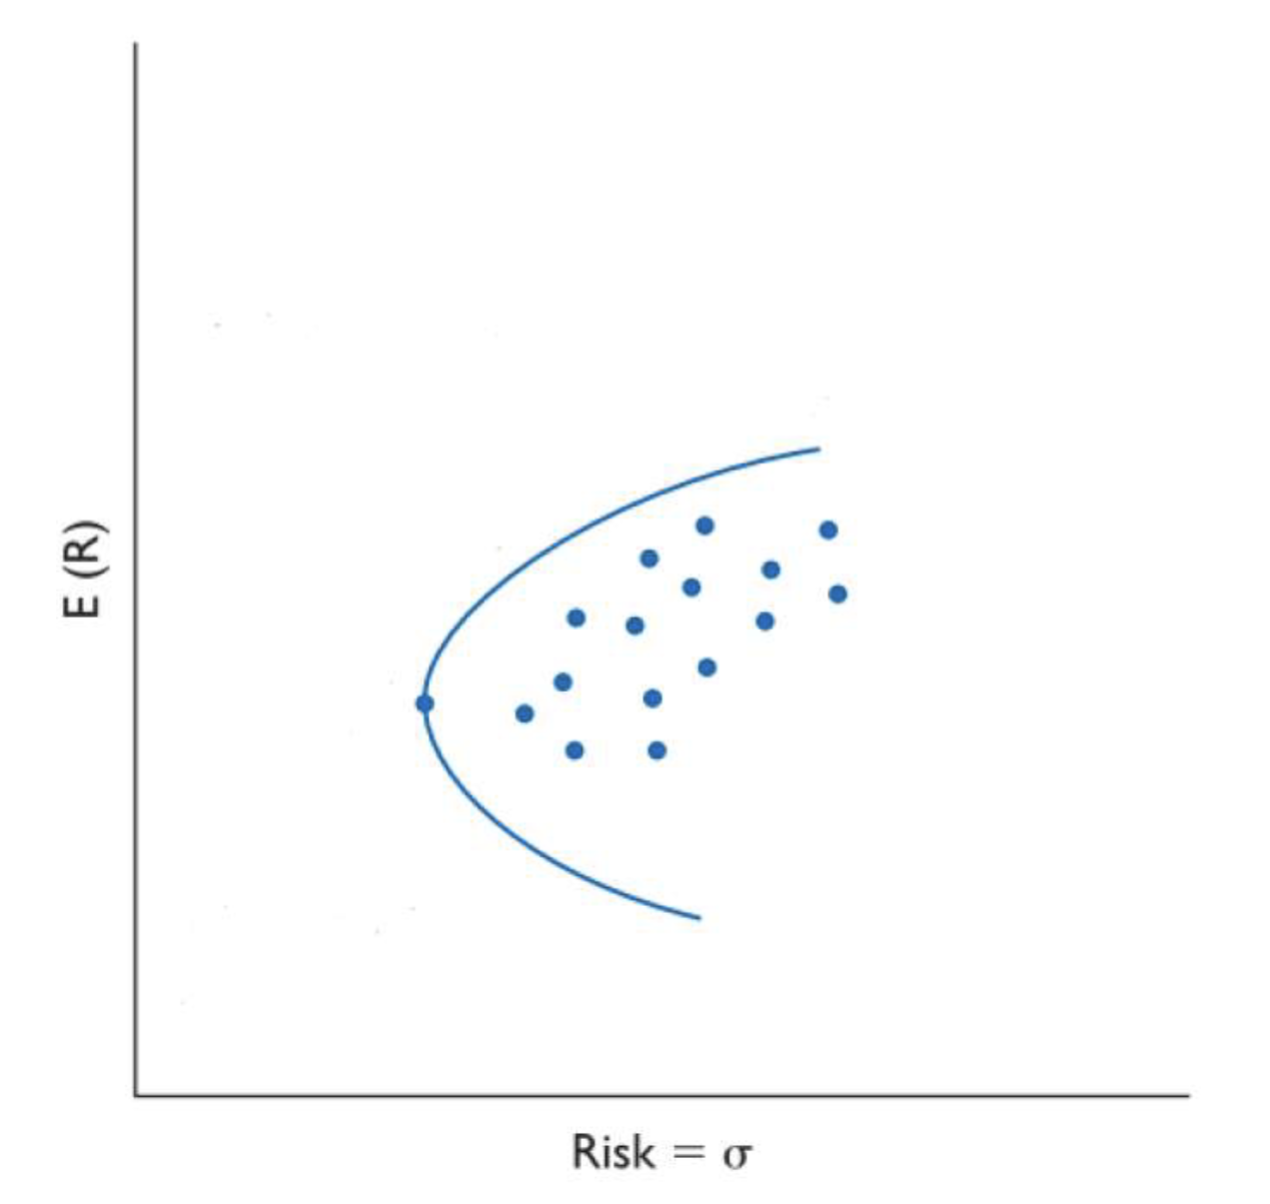
\includegraphics[scale=0.15]{9.png}
     \caption{Sammenhæng mellem risiko og afkast}
     \label{Figur 2}
\end{figure} 

En portefølje siges at være \textbf{domineret}, hvis der findes en
anden mulig portefølje med (1) samme forventede afkast, men lavere risiko eller (2) samme risiko, men højere forventet afkast. En portefølje er \textbf{efficient}, hvis den ikke er domineret. Det gælder, at en risikoavers investor aldrig ville vælge en domineret portefølje, hvorfor vi kan fokusere på de efficiente porteføljer. Den mulige portefølje med lavest risiko kaldes for \textbf{minimumsvariansporteføljen} ('global minimum variance portfolio'). Punkterne fra minimumsvariansporteføljen og \textit{op} kaldes for den efficiente rand, og indebærer netop alle efficiente porteføljer. Det er illustreret i nedenstående figur: 

\begin{figure}[h]
     \centering
     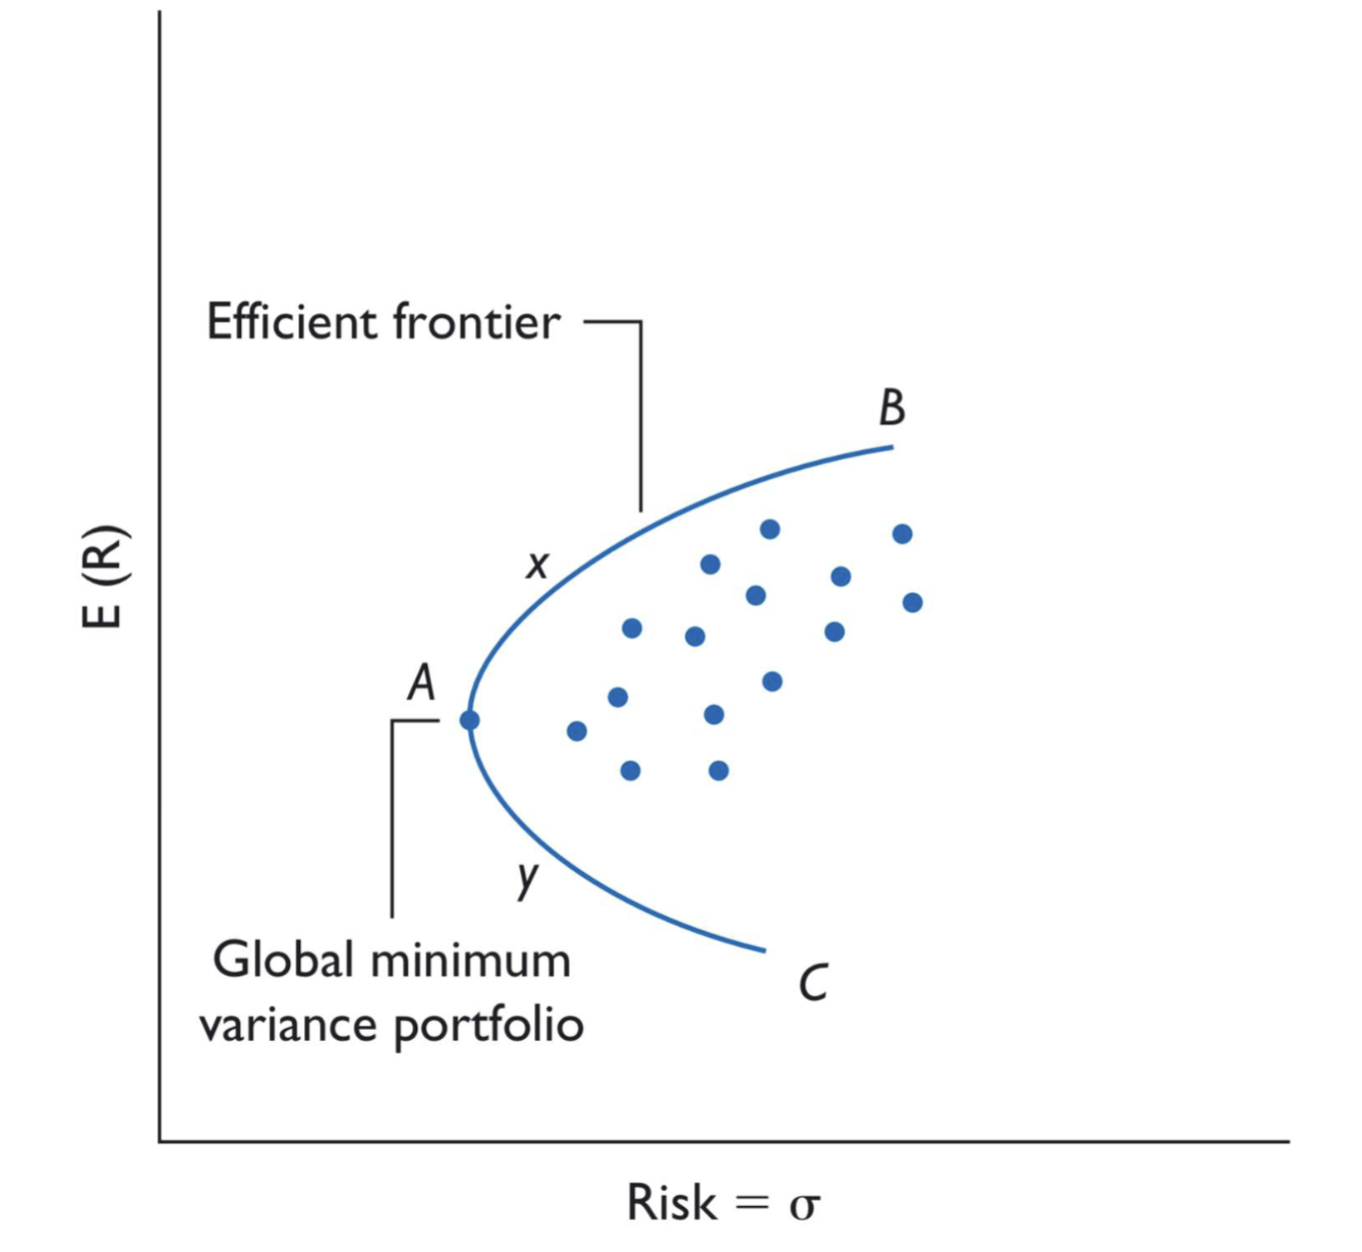
\includegraphics[scale=0.25]{10.png}
     \caption{Den efficiente rand og minimumsvariansporteføljen}
     \label{Figur 2}
\end{figure} 

For at afgøre, hvilken porteføljen en given investor bør vælge, indtegnes vedkommendes indifferenskurver, hvorefter tangeringen mellem den højest beliggende og den efficiente rand angiver den optimale portefølje for investoren. Det er illustreret nedenfor: 

\begin{figure}[h]
     \centering
     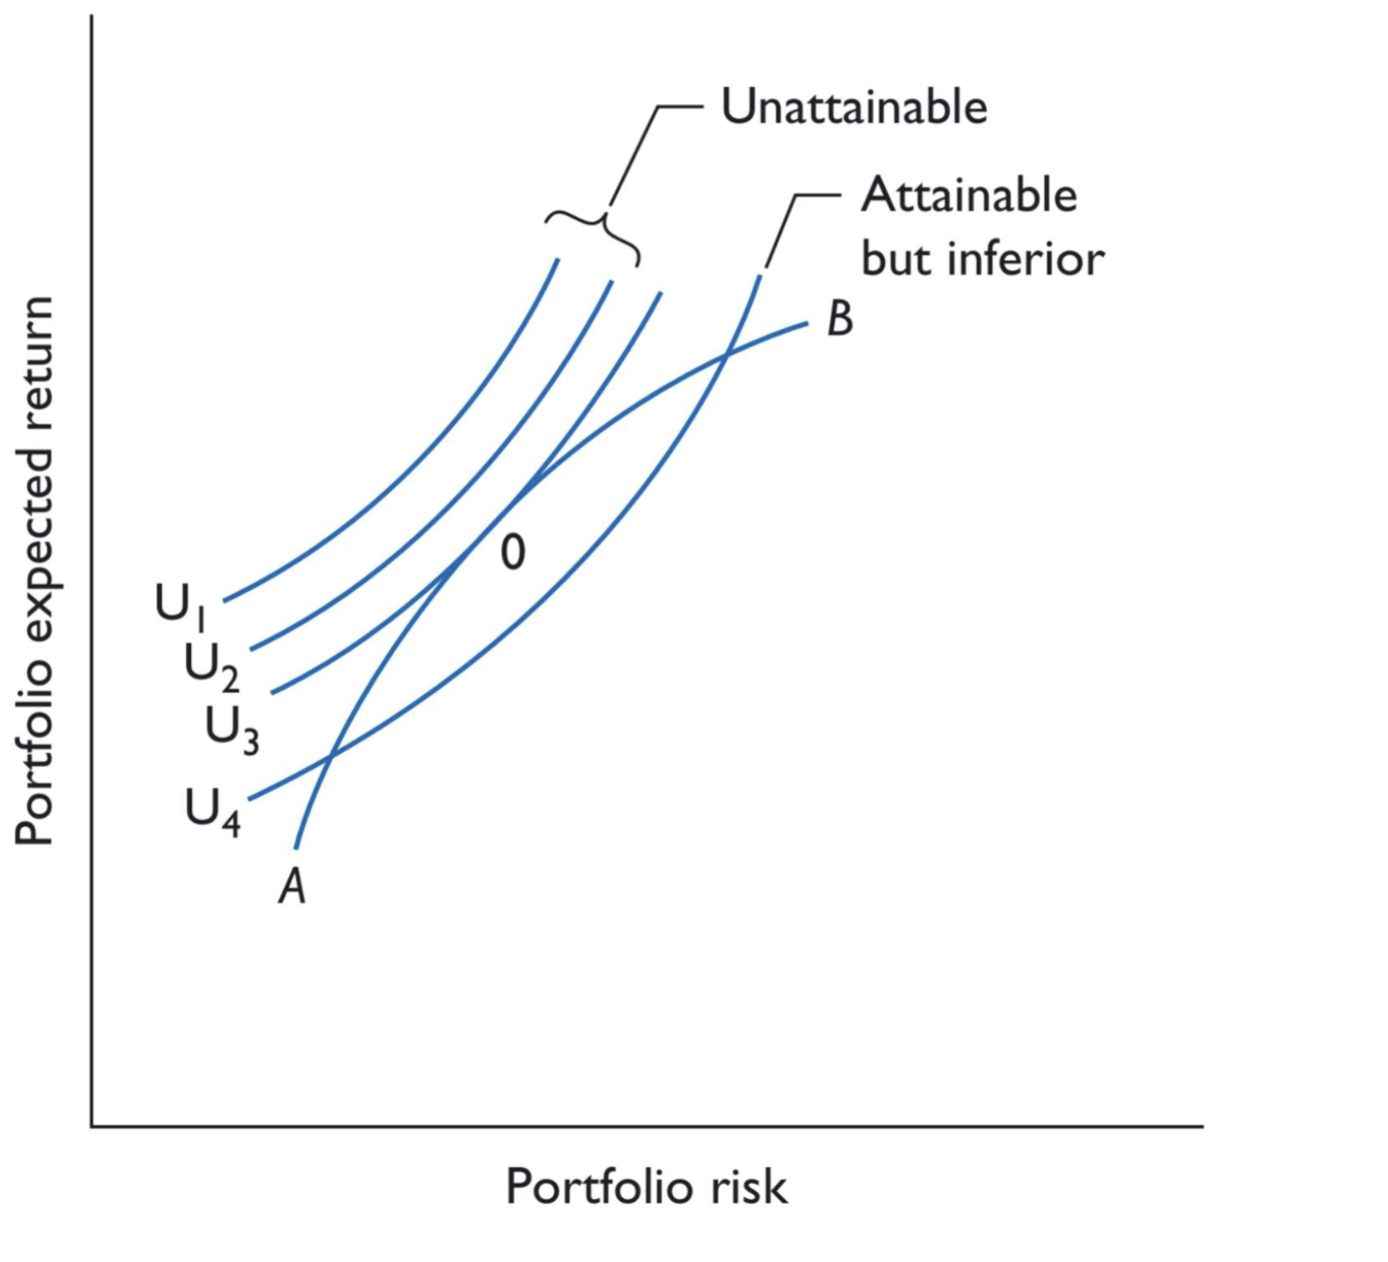
\includegraphics[scale=0.25]{11.png}
     \caption{Investorens præferencer vist ved indifferenskurver (1)}
     \label{Figur 2}
\end{figure} 

En investor, der er \textbf{risiko neutral vil have en flad indifferenskurve}, idet vedkommende blot vil opnå et givent afkast og således er \textit{ligeglad} med risiko. Vedkommende vil derfor også altid placere sig højest på den efficiente rand. \textbf{En mere risikoavers investor vil have en stejlere indifferenskurve}, idet vedkommende i højere grad skal kompenseres med øget afkast for at vælge højere risiko, mens en \textbf{mindre risikoavers investor vil have en mere flad indifferenskurver}, fordi vedkommende netop kræver mindre kompensation, i form af øget afkast, for større risiko. 

\begin{figure}[h]
     \centering
     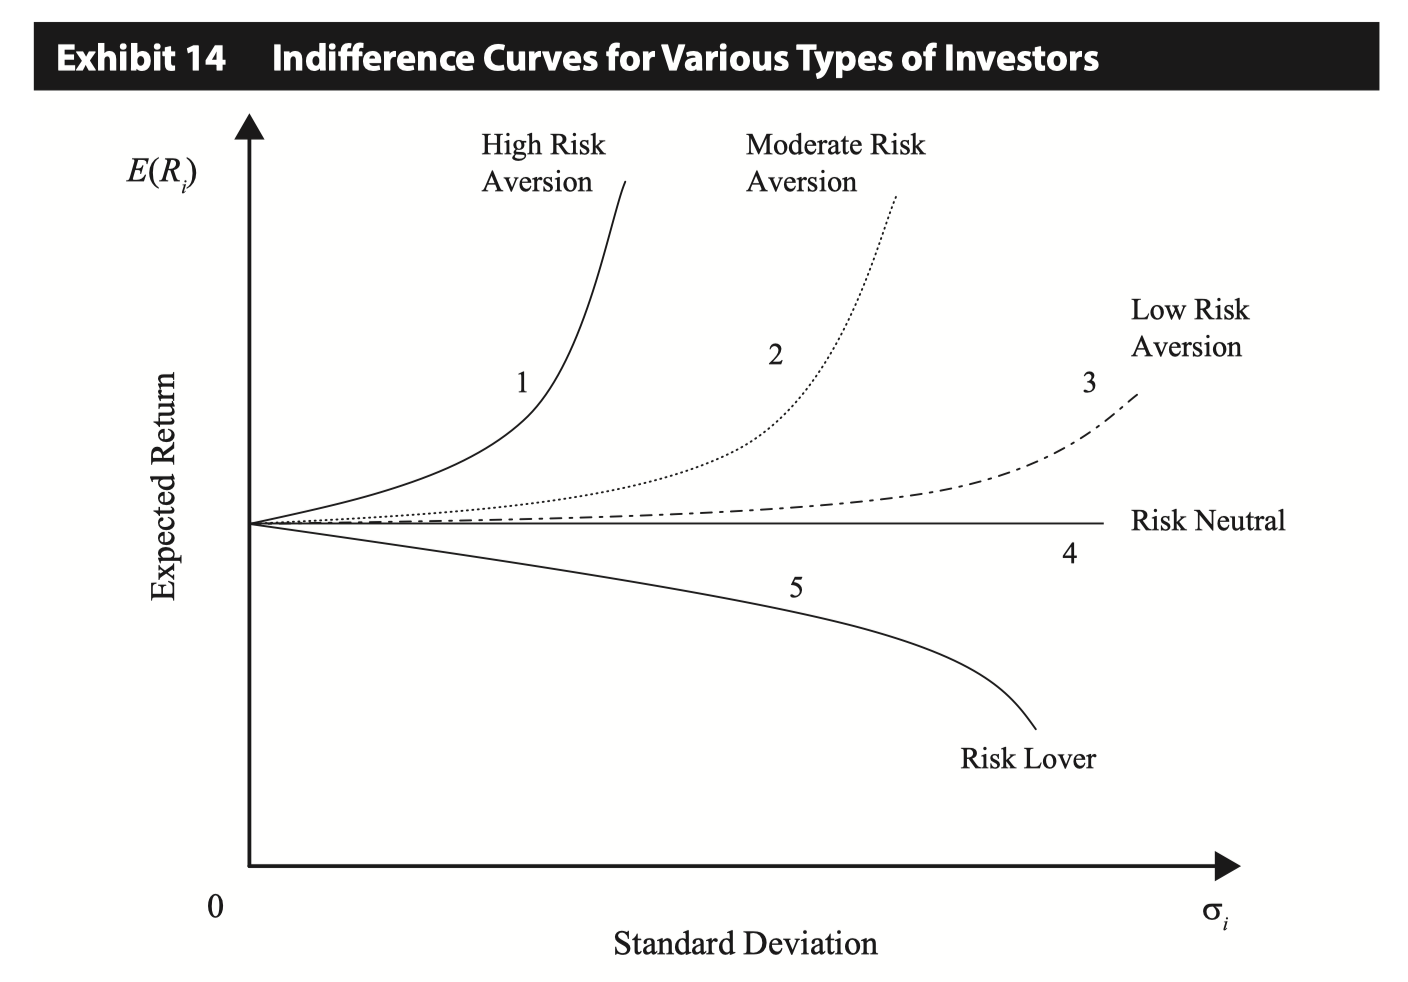
\includegraphics[scale=0.35]{12.png}
     \caption{Investorens præferencer vist ved indifferenskurver (2)}
     \label{Figur 2}
\end{figure}

De vigtigste indsigter fra porteføljeteorien er: 

\begin{itemize}
    \item \textbf{Indsigt 1:} En porteføljes varians kan reduceres, uden at det forventede afkast mindskes, ved at sprede investeringen over flere værdipapirer $\rightarrow$ \textit{diversifikationsprincippet}.
    \item \textbf{Indsigt 2:} Diversifikationsgevinsten er større, jo mindre \textit{korrelationen} mellem værdipapirerne i porteføljen er.
    \item \textbf{Indsigt 3:} Når porteføljen består af mange værdipapirer, afhænger dens varians primært af værdipapirernes indbyrdes \textit{kovarians}, og ikke af deres individuelle varianser.
    \item \textbf{Indsigt 4:} Ved at tilføje tilstrækkelig mange værdipapirer til porteføljen kan risiko fra individuelle virksomhedsforhold (\textit{variansled}) elimineres, men risiko fra markedsforhold (\textit{kovariansled}) kan ikke elimineres. Idiosynkratisk risiko kan elimineres, systematisk risiko kan \textbf{IKKE} elimineres.
\end{itemize}

\subsection{Evaluering af porteføljeteori}
Porteføljeteori kan opfattes — og dermed evalueres — som en \textbf{positiv} og \textbf{normativ} teori. Det gælder da;

\begin{enumerate}
    \item Modellen kan ses som en normativ teori for, hvordan investorer bør investere deres midler, såfremt modellens antagelser (herunder om risikoaversion) er opfyldt $\rightarrow$ Evaluer modellen ved at diskutere gyldigheden af dens antagelser og resultaternes praktiske anvendelighed
    \item Modellen kan ses som en positiv teori for, hvordan investorer rent faktisk investerer. $\rightarrow$ Evaluer modellen ved at diskutere gyldigheden af dens antagelser og ved at teste, om dens forudsigelser er i overensstemmelse med empiriske observationer
\end{enumerate}


\textbf{Begrænsningerne ved porteføljeteorien (Markowitz modellen) som en normativ teori} er: 

\begin{itemize}
    \item Ikke retvisende guide for investorer med andre præferencer end antaget i modellen
    \item Antager ingen risikofrie aktiver (se hvordan det ændrer resultaterne i CAPM)
    \item Forudsætter kendskab til et meget stort antal parametre (mange kovarianser!)
    \item Stor mængde af efficiente porteføljer $\rightarrow$ ingen præcis angivelse af, hvilken én man bør vælge
\end{itemize}

Mens \textbf{begrænsningerne ved porteføljeteorien som en positiv teori} er: 


\begin{itemize}
    \item Antager, at investorer udelukkende går op i porteføljens forventede afkast og varians
    \begin{itemize}
        \item Det behøver ikke være tilfældet i praksis
        \item EX: Tager ikke højde for at investorer i dag har præferenser over ESG parametre.
    \end{itemize}
    \item Forudsiger stort omfang af internationale investeringer, fordi værdipapirer er mindre korrelerede mellem lande end indenfor lande
    \begin{itemize}
        \item I praksis meget færre udenlandske aktier i porteføljer end teorien foreskriver (\textit{“home bias”})
    \end{itemize}
    \item Forudsiger høj grad af diversifikation blandt alle investorer
    \begin{itemize}
        \item Tegn på alvorlig underdiversificering blandt nogle private investorer
    \end{itemize}
\end{itemize}

\section{Kapitalmarkedsteori}
Kapitalmarkedsteorien også kendt som 'The Capital Asset Pricing Model' (CAPM) anvender porteføljeteorien til at analysere et marked med mange
forskellige investorer. I CAPM antager man: 

\begin{enumerate}
    \item Mulighed for at investere i et risikofrit aktiv (NYT!)
    \item Alle investorer bruger samme sandsynlighedsfordeling for afkast $\rightarrow$ samme opfattelse af forventede afkast, varianser og kovarianser
    \item Alle investorer har samme tidshorisont på én periode
    \item Alle investorer er små i forhold til det samlede marked $\rightarrow$ "pristagere"
    \item Ingen transaktionsomkostninger, skatter eller inflation
\end{enumerate}

\subsection{Det risikofrie afkast}
I modsætning til porteføljeteorien, vil vi i CAPM antage, at investorerne har mulighed for at investere i et risikofrit afkast (f.eks. en statsobligation). I praksis er der en kreditrisiko på statsobligationer, som vi dog ser bort fra. Den effektive rand får altså nu \textit{tilføjet} et punkt, der angiver et givent afkast, $R_F$ til en risiko på 0 (som illustreret nedenfor). 

\begin{figure}[h]
     \centering
     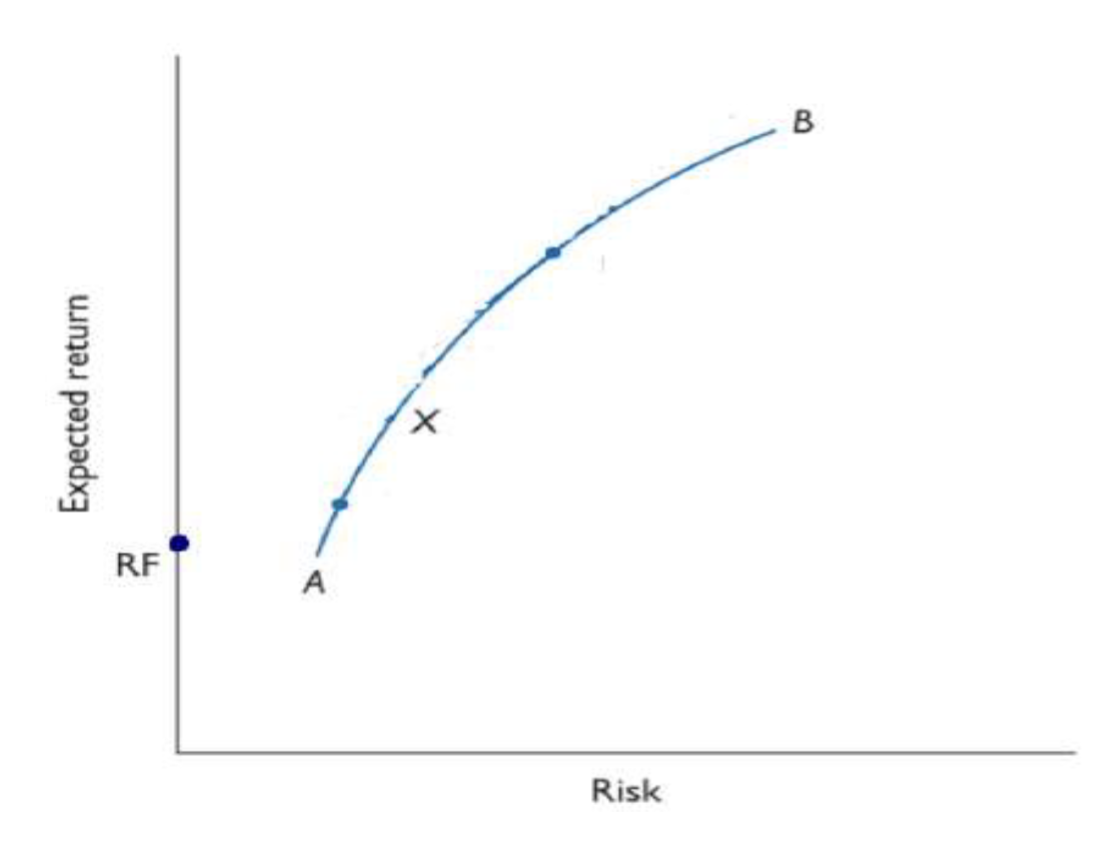
\includegraphics[scale=0.35]{13.png}
     \caption{Den efficiente rand med risikofrit afkast}
     \label{Figur 2}
\end{figure} 

En portefølje med to aktiver, $X$ og $Y$, hvor $Y$ er en risikofri obligation, hvor $\sigma = 0$ og $R=R_F$, vil således have et forventet afkast på $w_X E[R_X] + (1-w_x) R_F$, en standardafvigelse og $w_X \sigma_X$. Forskellige vægte af $w_X$ vil således blot give en ret linje gennem punkterne (0, $RF$) og ($\sigma_X, E[r_x]$). Formaliseret har vi altså, at: 
\begin{align*}
     E[R_Z] &= (1 - w_X) RF + w_X E[R_X] \\
     \sigma_Z &= w_X \sigma_X 
\end{align*}

Mens ligningen for den rette linje er: 

    \begin{equation}
    E(R_Z) = RF + \frac{E(R_X) - RF}{\sigma_X} \sigma_Z
    \end{equation}

Hvor hældningen er: 

 \begin{equation}
    E(R_Z)' =  \frac{E(R_X) - RF}{\sigma_X} 
    \end{equation}

Fortolkningen er, at det forventede afkast af en portefølje, $Z$, er et risikofrit afkast, $R_F$, plus en risikopræmie. Det er illustreret nedenfor; 

\begin{figure}[h]
     \centering
     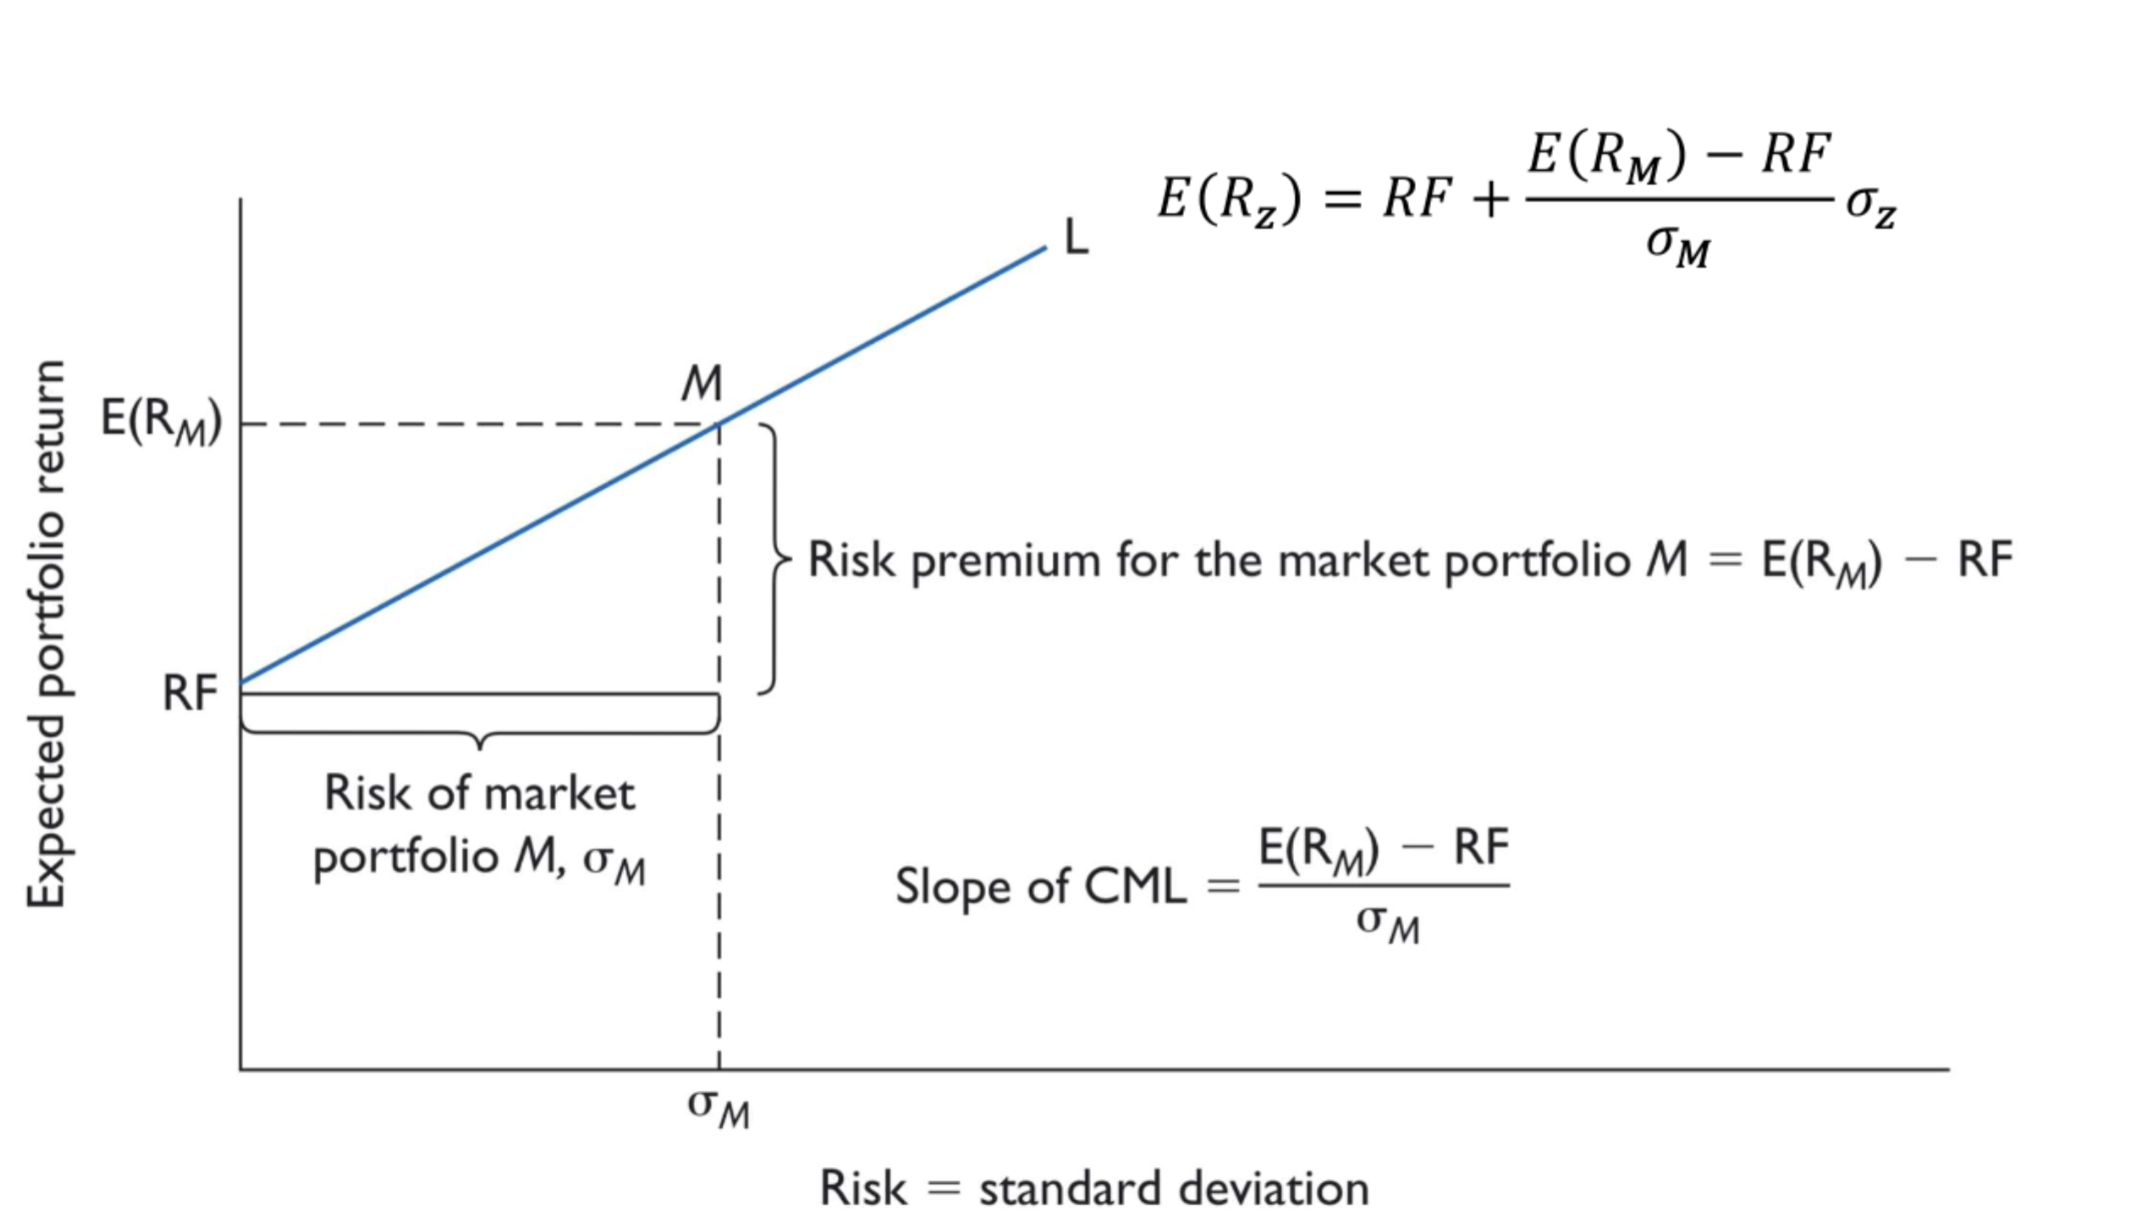
\includegraphics[scale=0.25]{16.png}
     \caption{Risikopræmie for kapitalmarkedslinjen}
     \label{Figur 2}
\end{figure} 

Investoren vil nu fir kunne vælge, hvordan han kombinerer det risikofrie afkast med forskellige porteføljer. Kombinationen med $X$ vil dog være domineret af kombinationen med $V$, hvorfor den optimale sammesætning er givet ved sekanten, der passerer punktet  og (0, $RF$) og ($\sigma_M, E[r_M]$). Porteføljen $M$ benævnes \textbf{tangentporteføljen}.

\begin{figure}[h]
     \centering
     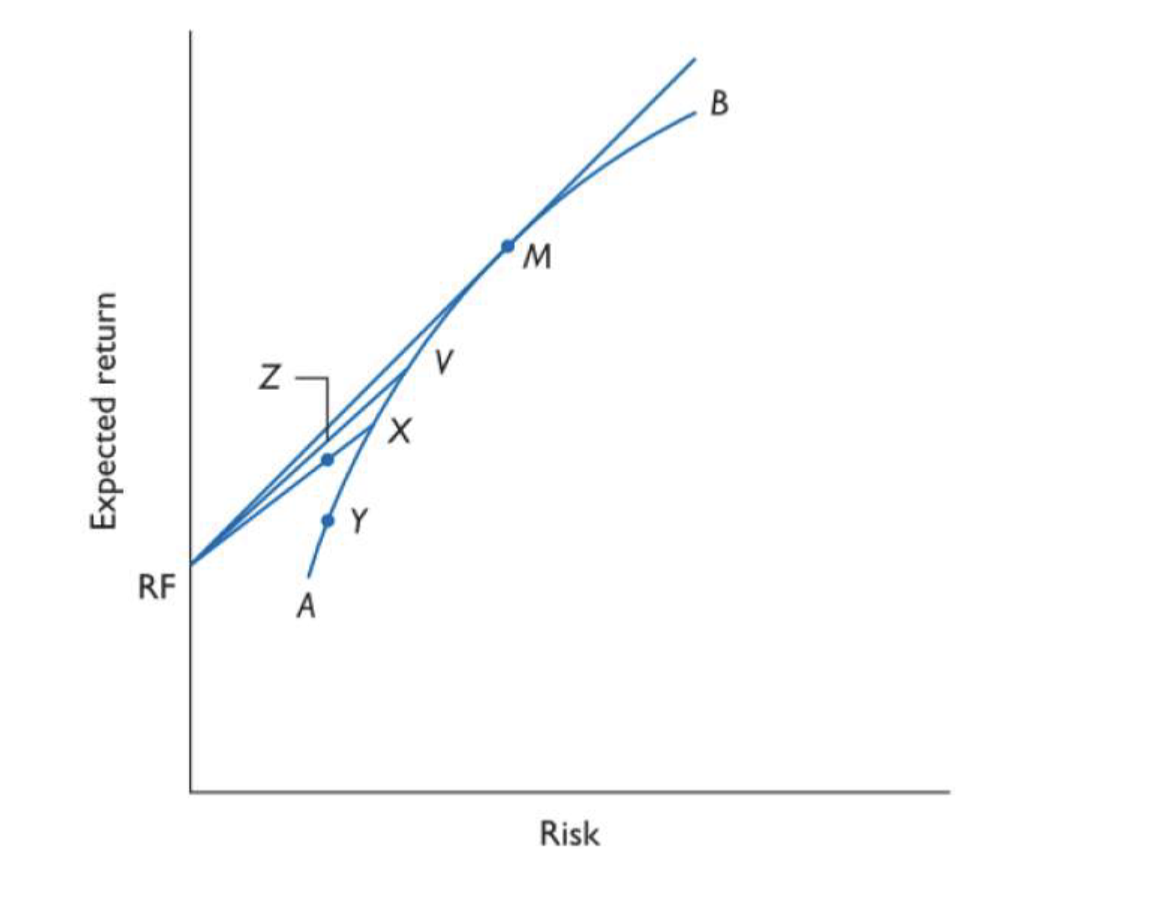
\includegraphics[scale=0.35]{14.png}
     \caption{Udledning af kapitalmarkedslinjen}
     \label{Figur 2}
\end{figure} 


\newpage
Mængden af efficiente porteføljer ligger nu på en ret linje gennem det
risikofri aktiv og tangentporteføljen, der kaldes for \textbf{kapitalmarkedslinjen}. Selvom investorerne har forskellige præferencer, vil alle (optimalt set) vælge en portefølje som består af en andel af det risikofri aktiv samt en andel af markedsporteføljen. En investor med høj risikoaversion vil vælge en lav andel af $M$, mens en investor med høj risikoaversion vil vælge en en høj andel af $M$. Hvis er meget risikoavers, og benytter sig af gearing, vil $M>1$ og andelen af det risikofri aktiv vil være mindre end 1, hvorfor vedkommende skal låne til markedsrenten og en lavere risikofri rente således er at foretrække for vedkommende. To investorers indifferenskurver, samt kapitalmarkedslinjen, er vist nedenfor:  

\begin{figure}[h]
     \centering
     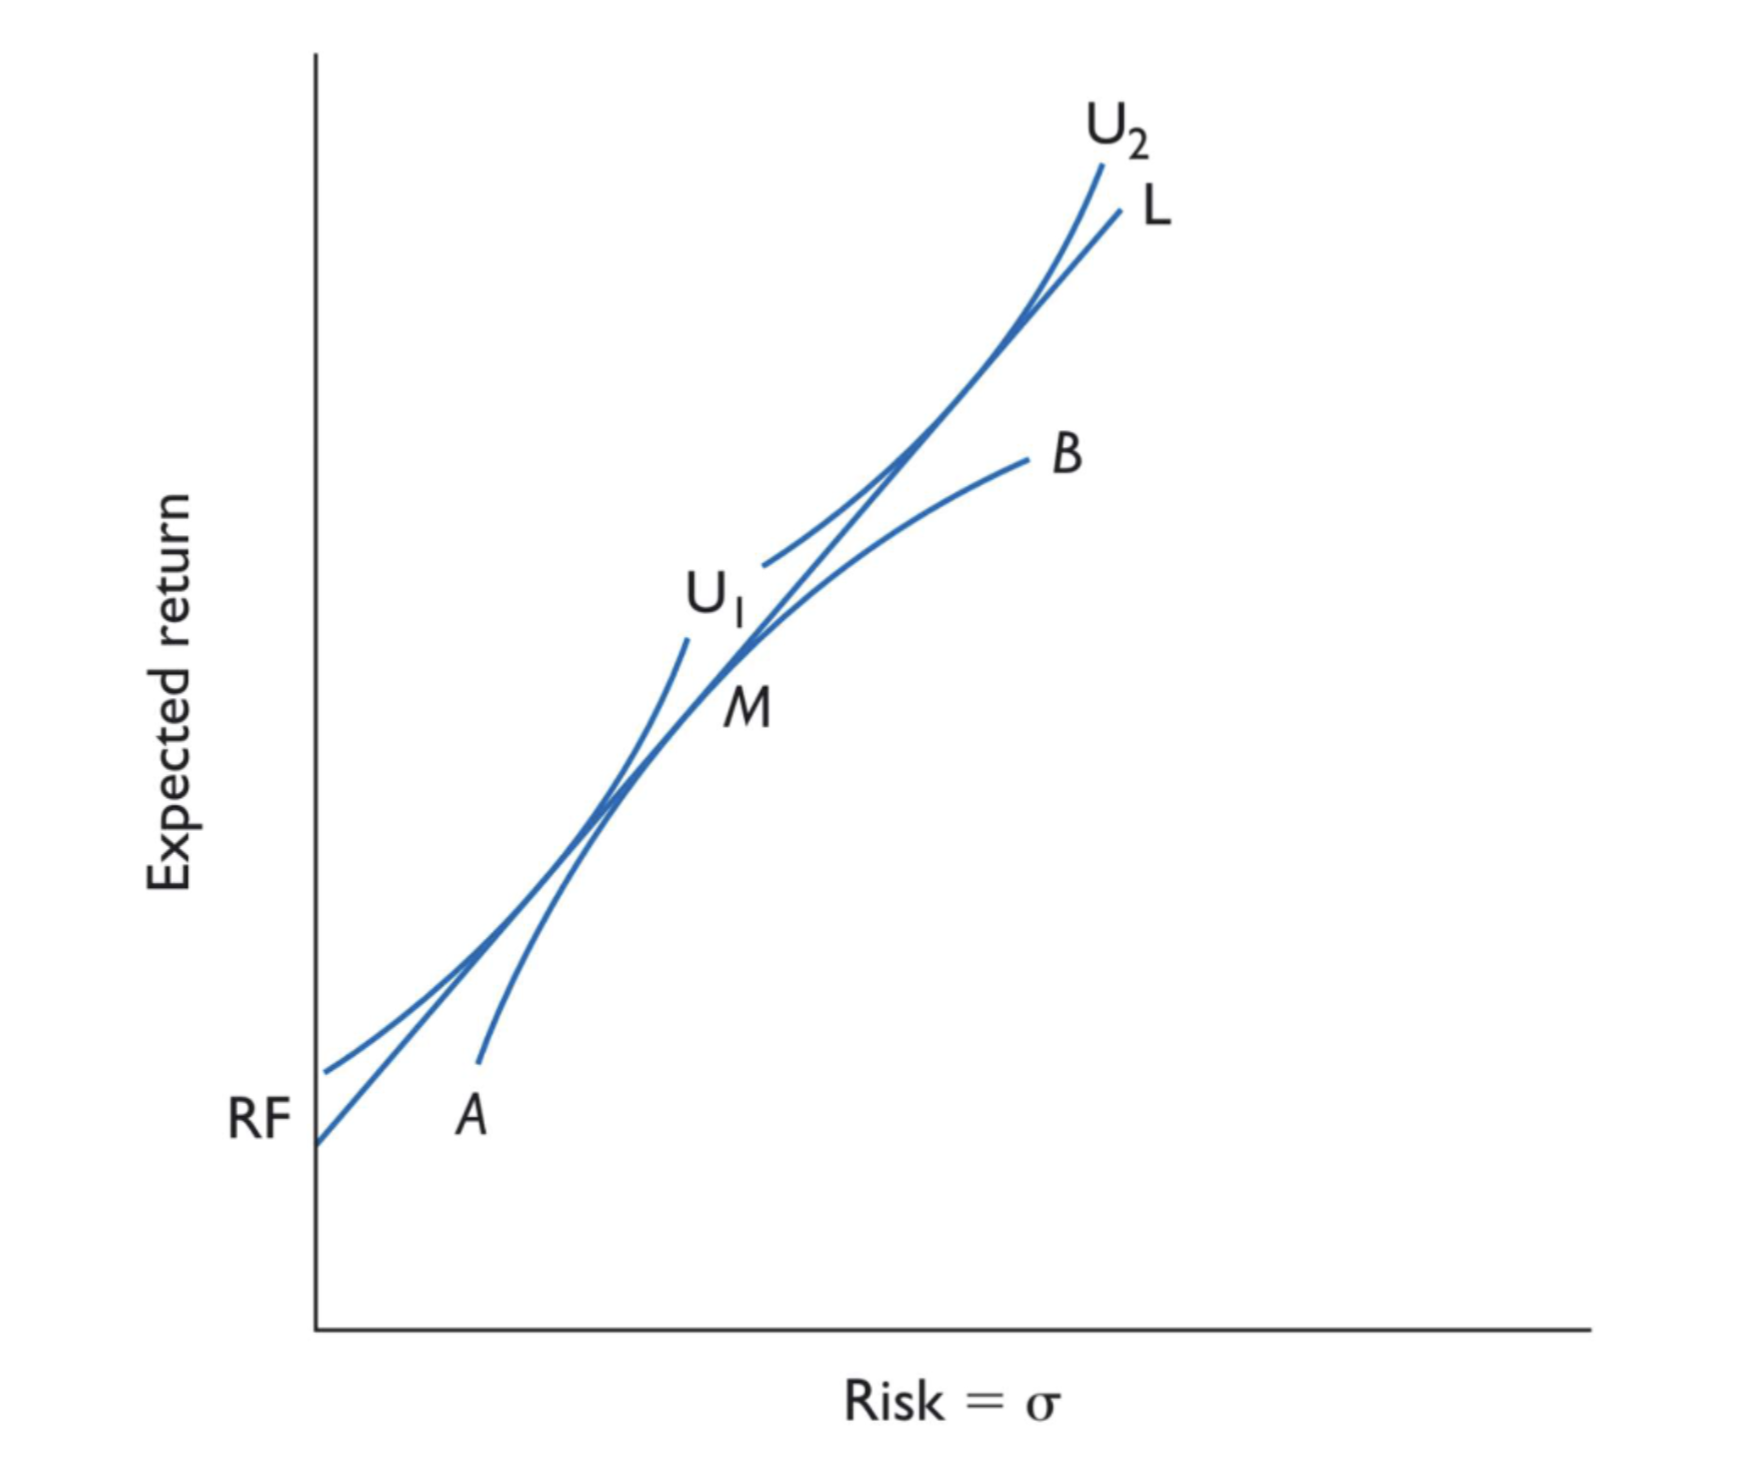
\includegraphics[scale=0.25]{15.png}
     \caption{Kapitalmarkedslinjen med forskellige indifferenskurver}
     \label{Figur 2}
\end{figure} 

\subsection{Markedsporteføljen ($M$)}
Modellen forudsiger, at alle investorer bruger en del af deres formue på det risikofrie aktiv og en del på markedsporteføljen, $M$. Det gælder, at markedsporteføljen består af alle risikofyldte aktiver på markedet, og at vægten for hvert aktiv er givet ved dens andel af markedets samlede værdi. Betragt tre aktier med tilhørende markedsværdier $A=30, B=20, C=50$. Så vil vægtene være givet ved $w_A=\frac{30}{100}=0,3$, $w_B=\frac{20}{100}=0,2$ $w_C=\frac{50}{100}=0,5$. Årsagen til, at alle værdipapirer er inkluderet følger af simpel mikroteori. Antag, at der findes et værdipapir, der ikke er inkluderet i markedsporteføljen, $M$. Det betyder, at ingen investorer køber værdipapireret og at kursen falder. Når kursen falder stiger afkastet, hvilket øger efterspørgslen, indtil alle har inkluderet aktien og der igen har indfundet sig en ligevægt på markedet. 

\subsection{Prisen på enkelte værdipapirer ($\beta$)}
For at besvare spørgsmålet om, hvor højt et forventet afkast investorerne vil kræve for at indlemme et givet værdipapir i markedsporteføljen?, skal vi undersøge, hvordan det givne værdipapir påvirker markedsporteføljens forventede afkast og risiko. Det skyldes, at investorerer har præferencer over deres samlede portefølje, men ikke over de enkelte værdipapirer. Et estimat for, hvordan den samlede risiko af markedsporteføljen påvirkes ved at indlemme et nyt værdipapir $i$ er givet ved: 

\begin{equation}
    \beta_i = \frac{\text{Cov}_{i,M}}{\sigma_M^2}
\end{equation}

hvor $\beta_i$ og målet er skaleret med markedsporteføljens samlede risiko, 
$\sigma_M^2$. Beta udtrykker således \textbf{relevante risiko} ved værdipapir $i$ for en investor, som i forvejen har investeret i markedsporteføljen. Risikoen afhænger netop af \textbf{samvariationen med markedsporteføljen}. Idet korrelationskoefficienten er givet ved: $\rho_{XY} = \frac{\text{Cov}_{X,Y}}{\sigma_X \sigma_Y}$, kan formel 75 omskrives til: 

   \begin{equation}
        \beta_i = \frac{\text{Cov}_{i,M}}{\sigma_M^2} = \frac{\rho_{i,M} \cdot \sigma_i \sigma_M}{\sigma_M^2} = \rho_{i,M} \cdot \frac{\sigma_i}{\sigma_M}
    \end{equation}

$\beta$ udtrykker altså en kombination af to ting: (1) hvor meget afkastet på værdipapiret varierer i forhold til afkastet på markedsporteføljen \(\left( \frac{\sigma_i}{\sigma_M} \right)\), og (2) hvor korreleret dets afkast er med markedsporteføljens \(\left( \rho_{i,M} \right)\). Individuelle værdipapirer vil typisk have: 

\begin{itemize}
    \item Større variabilitet i afkastet end markedsporteføljen $\sigma_i > \sigma_M$
    \item Positiv korrelation med markedsporteføljen, $0<P_{i,M}<1$
\end{itemize}

For individuelle værdipapirer gælder derfor at \( \beta_i \) kan være:
\begin{itemize}
        \item \textit{Mindre end 1} : Mindre risiko end markedet
        \item \textit{Lig med 1} : Samme risiko som markedet
        \item \textit{Større end 1} : Større risiko end markedet
\end{itemize}

Det gælder helt generelt, at jo højere $\beta$, jo højere forventet afkast vil investorerne kræve for at inkludere den givne aktie i deres markedsportefølje. Den centrale ligning, der her ikke vil udledes, er: 

\begin{equation}
    \textit{Krav til forventet afkast af værdipapir i} = RF + \beta_i \cdot (E[R_M] - RF)
\end{equation}

hvor $RF$ er det risikofri afkast, $E[R_M] - RF$ er markedsrisikopræmien og Risikopræmien for værdipapir $i$ er $\beta_i \cdot (E[R_M] - RF)$. \textbf{Værdipapirmarkedslinjen} angiver sammenhængen mellem $\beta$ og kravet til det forventede afkast og er positivt hældende, svarende til, at højere $\beta$-værdi fører til et højere krav til det forventede afkast. 

\begin{figure}[h]
     \centering
     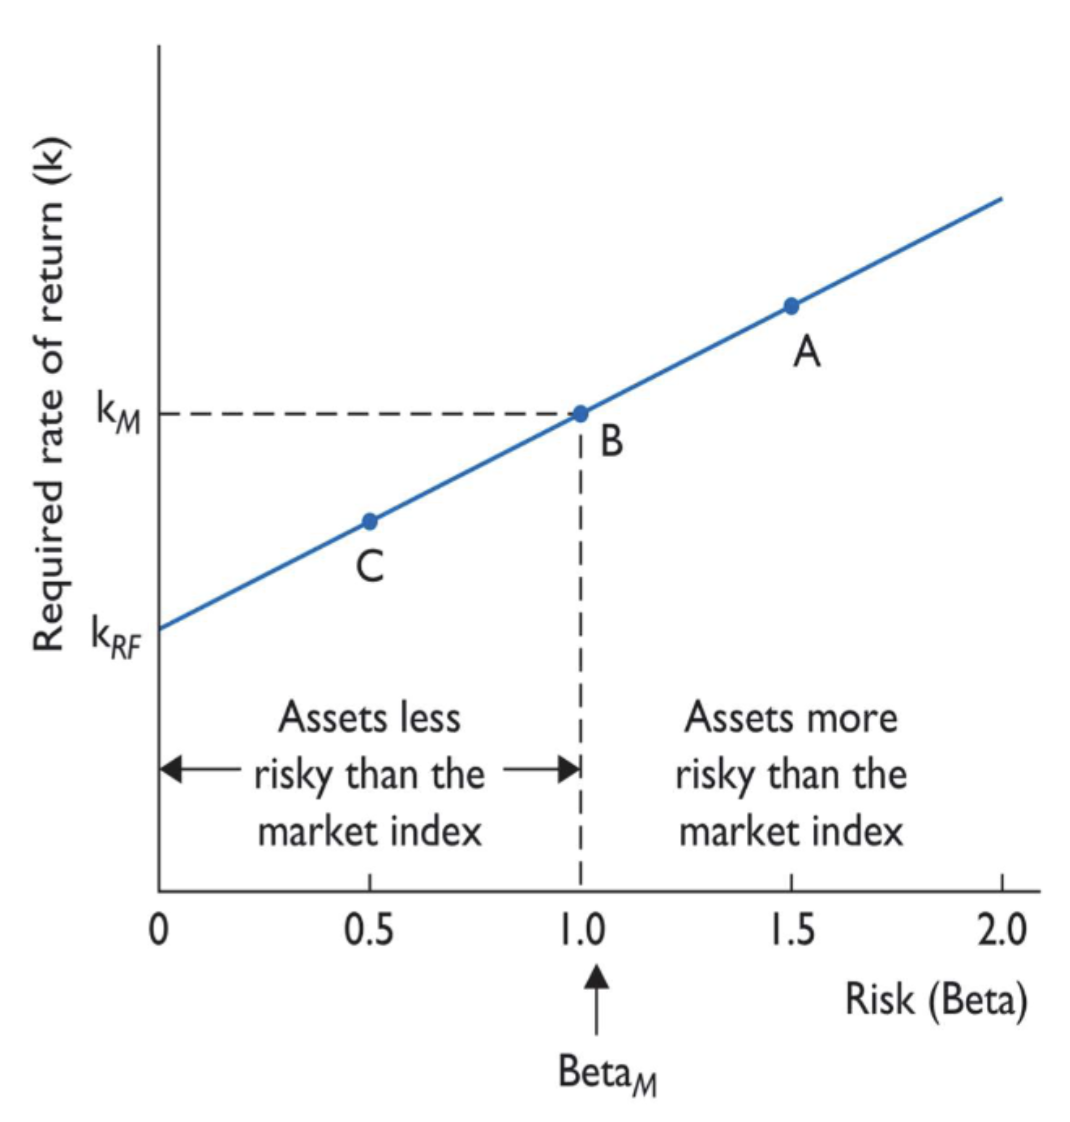
\includegraphics[scale=0.45]{17.png}
     \caption{Værdipapirmarkedslinjen}
     \label{Figur 2}
\end{figure} 

\newpage

Hvor; 

\begin{itemize}
    \item Værdipapirer med \( \beta_i < 1 \) har mindre risikopræmie end markedsporteføljen $\rightarrow$ krav til forventet afkast lavere end markedsporteføljens forventede afkast
    \item Værdipapirer med \( \beta_i > 1 \) har større risikopræmie end markedsporteføljen $\rightarrow$ krav til forventet afkast større end markedsporteføljens forventede afkast
\end{itemize}

En aktie kan dermed godt have et \textbf{negativ krævet afkast}, hvis den kan reducere den samlede risiko tilstrækkelig meget! 

\vspace{10 pt}

Betragt en situation, hvor det risikofrie afkast er givet ved 5 pct. og det forventede markedsafkast er 10 pct. En aktie med hhv. $\beta = 0,5$ og $\beta = -3$  må altså have følgende forventede afkast for at kunne sælges: 
\begin{align*}
    E[R_i] &= 10 + 0,05 \cdot (10-5) = 7,5 \% \\
    E[R_i] &= 10 -3 \cdot (10-5) = -5 \% 
\end{align*}

Årsagen til, at ethvert værdipapir ligger på linjen, dvs. det forventede afkast netop opfylder afkastkravet beskrevet i formel 77 er, kan ligeledes forklares ud fra mikro teori. 

\begin{itemize}
    \item Hvis \( E[R_i] > RF + \beta_i \cdot (E[R_M] - RF) \)
    \begin{itemize}
        \item Papiret tilbyder et højere forventet afkast end dets risiko tilsiger $\rightarrow$ er undervurderet
        \item Investorerne ønsker at købe papiret $\rightarrow$ prisen stiger
        \item Dets forventede afkast falder (husk: \( TR = \frac{CF + P_E - P_B}{P_B} \))
    \end{itemize}
    \item Hvis \( E[R_i] < RF + \beta_i \cdot (E[R_M] - RF) \)
    \begin{itemize}
        \item Prisen falder, \( E[R_i] \) stiger
    \end{itemize}
\end{itemize}

\subsection{Estimation af beta ($\beta$)}
Beta kan empirisk estimeres ved: 

\begin{equation}
            \hat{\beta}_i = \frac{\widehat{\text{Cov}}_{i,M}}{\widehat{\sigma}_M^2}
\end{equation}

Hvor $\widehat{\text{Cov}}_{i,M}$ er den empiriske kovarians mellem afkastet på værdipapir $i$ og afkastet af markedsporteføljen, og $\widehat{\sigma}_M^2$ er den empiriske varians på afkastet af markedsporteføljen. 

\vspace{10 pt}

I praksis kan beta også estimeres ved at plotte afkastet ($TR$) af et værdipapir over en længere periode langs y-aksen og plotte afkastet ($TR$) af markedsporteføljens på x-aksen. Ved at estimere den bedste rette linjer vha. lineær regression og aflæse hældningen, har vi et estimat for $\beta$. Det skyldes, at hældningen af linjen netop viser, hvor meget værdipapirets afkast ændrer sig for hver ændring i markedsporteføljens afkast. Hældningen er således en direkte måling af forholdet mellem samvariationen af de to afkast (kovariansen) og markedsporteføljens varians. Eksempel 8 gennemgår et eksempel heraf

\begin{tcolorbox}[breakable, colback=red!5!white, colframe=red!50!black, title= Eksempel 8: Estimation af beta]
Betragt nedenstående data for afkast af en aktie og markedsindekset: 

\vspace{10 pt}
\begin{center}
        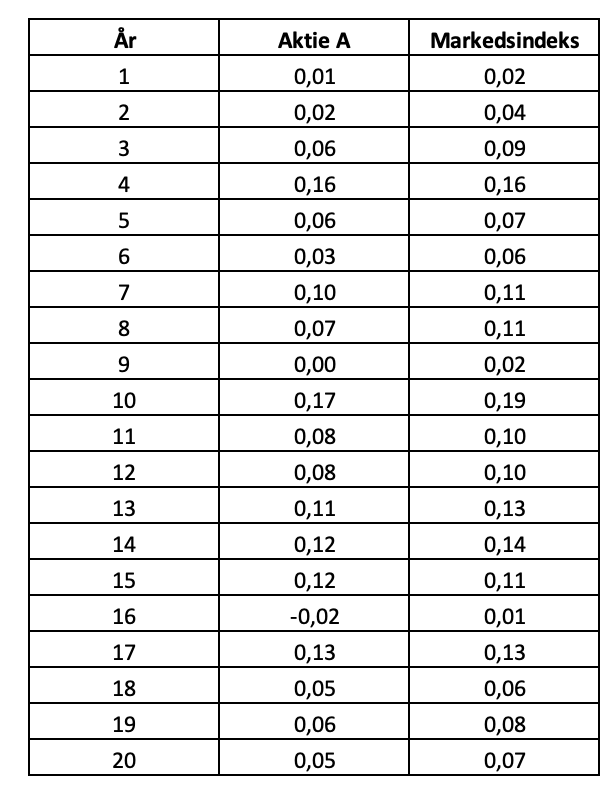
\includegraphics[width=0.45\textwidth]{18.png}
\end{center}

Aktie A's afkast plottes nu langs x-aksen, mens markedsindeksets afkast afsættes af andenaksen. Det ses, at beta her estimeres til ca. 0,88, mens den statistisk beregnede værdi er ca. 1,05.

\vspace{10 pt}
\begin{center}
        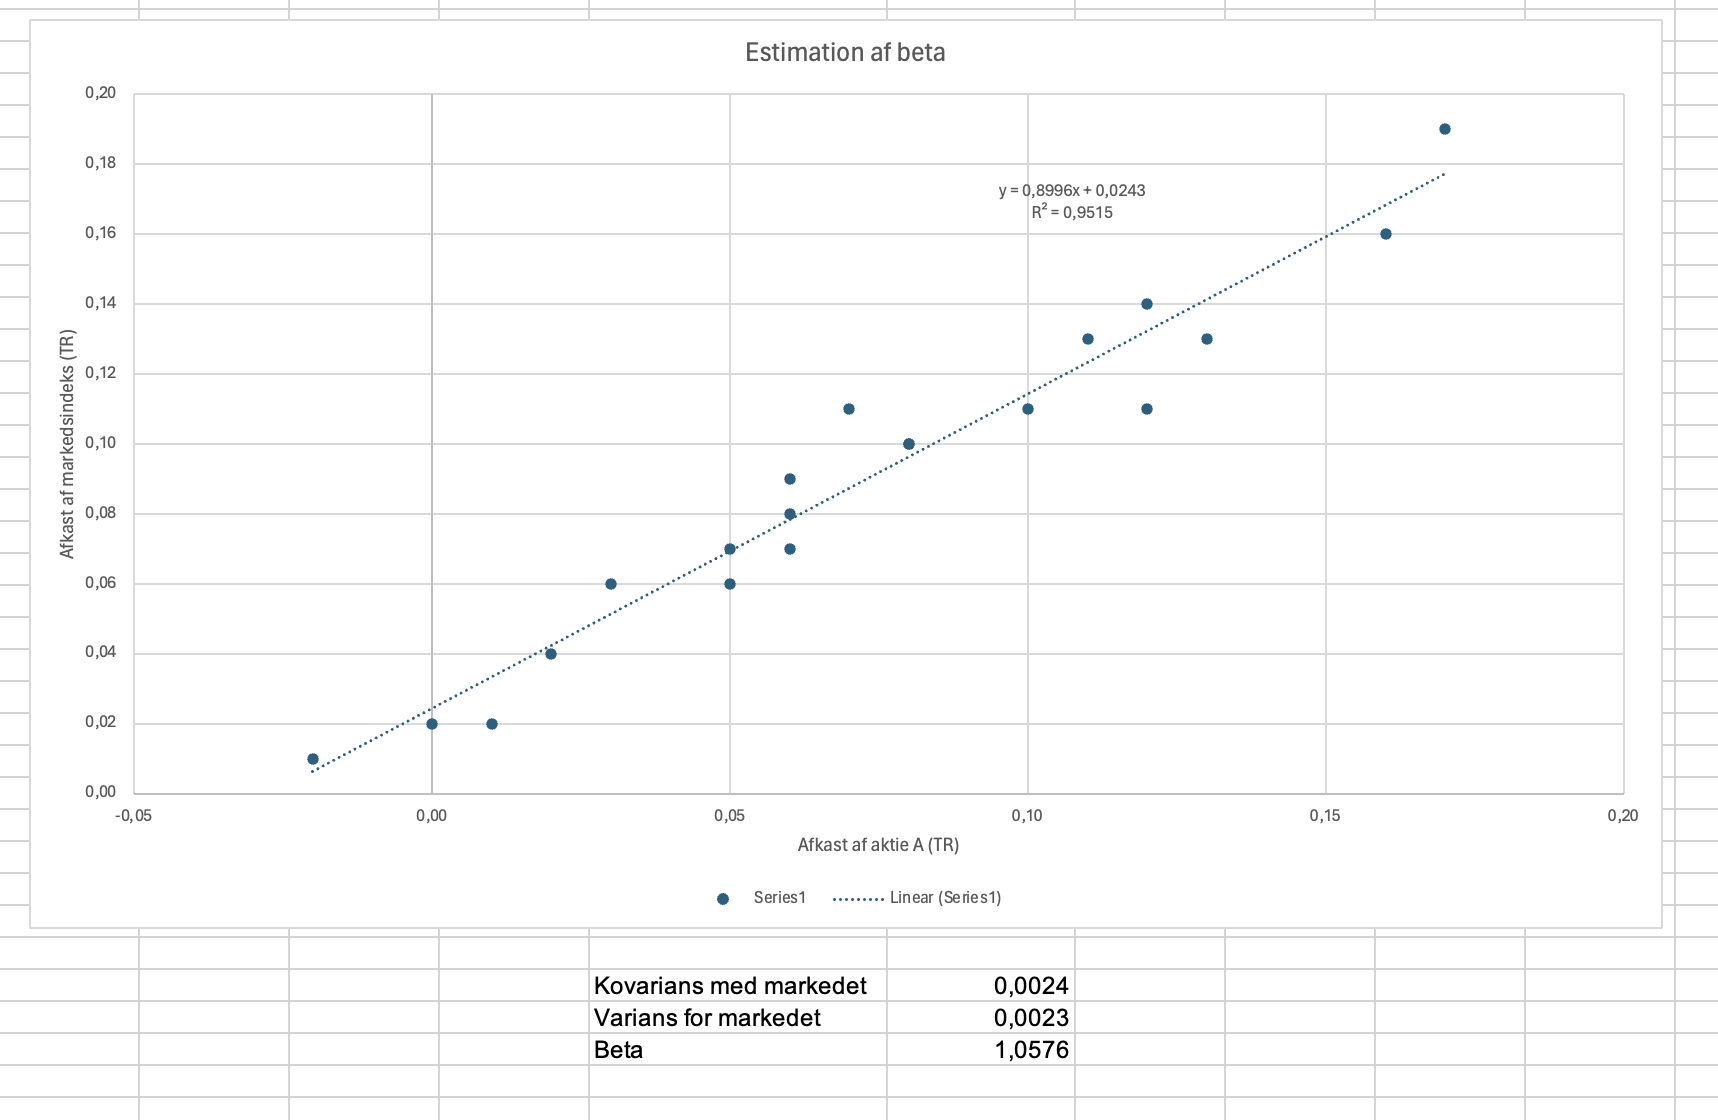
\includegraphics[width=0.85\textwidth]{19.png}
\end{center}
\end{tcolorbox}

\subsection{Empiriske udfordringer ved CAPM}
De vigtigste empiriske udfordringer ved CAPM — dvs. årsager til, at det faktiske afkast kan være anderledes end det afkast, som CAPM modellen forudsiger er bl.a, at; 

\begin{itemize}
    \item Investorerne benytter en anden sandsynlighedsfordeling med hensyn til afkast og risiko (standardafvigelse). 
    \item Investorerne inkluderer overvejelser omkring transaktionsomkostninger, herunder skatter, inflation og kurtage.
    \item Man ser empirisk at investorer har et \textit{home-bias} og dermed foretrækker at investere i indenlandske aktier. 
    \item Man ser empirisk, at investorerer ofte investerer i få værdipapirer (af uvisse årsager), hvorfor det ikke er repræsentativt at antage, at alle skulle investere i en markedsportefølje og at det krævede afkast afhænger, hvordan den givne aktie ændrer denne markedsportefølje. 
    \item Investorer kan have en længere tidshorisont end CAPM (der netop antager, at der kun er en periode). 
    \item Investoreren kan tage udgangspunkt i et andet risikofrit afkast, end det vi arbejder med i vores modeller (og det kan ændre sig over perioder!). 
    \item Investoren er i højere grad end modellen foreskriver det pristager, og kan således i mindre grad påvirke markedsfejl, herunder ikke perfekt information, der kan presse prisen (og dermed afkastet) på en aktie op eller ned.
\end{itemize}

\subsection{Gælds- og egenkapitalsfinansiering}
\textit{WACC} ('weighted average cost of capital') og udtrykker virksomhedens vægtede kapitalomkostning. Altså; hvor meget det koster for en virksomhed at finansiere sine aktiviteter. Det er defineret som: 

\begin{equation}
    WACC = x_{debt} \cdot k_{debt} + x_{equity} \cdot k_{equity}
\end{equation}

hvor $x_{debt}$ og $x_{equity}$ angiver andelen af gældsfinansiering og egenkapitalfinansiering, og $k_{debt}$ og $k_{equity}$ angiver virksomhedens gælds- og egenkapitalsomkostning. Årsagen til, at egenkapitalsfinansiering (økonomisk set) er en omkostning for virksomheden er, at finansiering med egenkapital giver nye investorer
ret til andel af overskud, hvilket betyder mindre udbytte til nuværende ejere, som netop er omkostningen ved egenkapitalfinansiering. Det gælder, at jo højere afkastkravet er, jo større en andel af fremtidigt overskud vil investorerer have del af, hvorfor der vil være en højere egenkapitalomkostning. \textbf{Selv hvis ejeren selv investerer midlerne vil egenkapitalsomkostningen dog ikke være 0}, idet der er en alternativomkostning forbundet med ejerens investering. Eksempel 9 gennemgår en beregning, der tydeliggører intuitionen bag ovenstående: 

\begin{tcolorbox}[breakable, colback=red!5!white, colframe=red!50!black, title= Eksempel 9: Forholdet mellem gælds- og egenkapitalsfinansiering]
Betragt et investeringsprojekt som vil give virksomheden et forventet afkast på 5 pct. af den investere sum (3 mio.) efter et år. Virksomheden har 1 mio. i egenkapital og kan vælge at finansiere de øvrige 2 mio. ved at optage gæld eller modtage indskud fra andre investorer. Hvis virksomheden vælger at gældsfinansiere projektet til en rente på $r$ bliver det forventede udbytte: 

\begin{equation*}
    3 \cdot 1,05 - (1+r) \cdot 2 = 3,15 - 2 - 2r = 1,15 - 2r
\end{equation*}

Mens det forventede afkast (TR) af 1 mio. (virksomhedsejernes indskud) bliver: 

\begin{equation*}
    \frac{1,15 - 2r - 1}{1} = 0,15 - 2r
\end{equation*}

Antag nu i stedet, at virksomhedsejeren vil finansiere projektet ved at sælge aktier, og der på starttidspunktet er 100 aktier, som hun ejer. De nye investorer kræver et afkast på $x$ for at investere i virksomheden. Det forventede udbytte per aktie er: 

\begin{equation*}
    \frac{3,15}{100} = 31.500 
\end{equation*}

Hvorfor det forventede afkast ved en købspris på $P$ bliver: 

\begin{equation*}
    x = \frac{31.500-P}{P} \Longleftrightarrow P = \frac{31.500}{(1+x)}
\end{equation*}

Antallet af aktier, der skal sælges til en pris $P$ for at opnå en finansiering på 2 mio. er altså; 

\begin{equation*}
    \frac{2.000.000}{\frac{31.500}{(1+x)}} \Longleftrightarrow \frac{2.000}{\frac{31,5}{(1+x)}} \Longleftrightarrow  \frac{2.000 \cdot (1+x)}{31,5}
\end{equation*}

Ejernes udbytte efter 1 år er nu afkastet per aktie, ganget med antallet af aktier, der er givet ved $100-\frac{2.000 \cdot (1+x)}{31,5}$. Dvs;
\begin{align*}
    &= 31.500 \cdot (100-\frac{2.000 \cdot (1+x)}{31,5}) \\
    & = 3.150.000 - 100 \cdot 2000 - 200x \\
    & = 1.150.000 - 2.000.000 \cdot r \\
    & =  1,15 [\text{mio.}] - 2 [\text{mio.}] \cdot r
\end{align*}

Hvor det forventede afkast (TR) for virksomhedsejeren er:

\begin{equation*}
    \frac{1,15 - 2r-1}{1} = 0,15 - 2r 
\end{equation*}

Hvilket netop er sammenfaldende som situationen, hvor virksomhedsejeren finansierede projektet gennem gæld. 
\end{tcolorbox}

Vi kan nu skabe en sammenhæng mellem CAPM og WACC ved at huske tilbage til CAPM, hvor kravet til det forventede afkast er:  

\begin{equation}
    \textit{Krav til forventet afkast af værdipapir i} = RF + \beta_i \cdot (E[R_M] - RF)
\end{equation}

Det følger heraf, at en virksomheds egenkapitalomkostning er stigende i betaværdien, idet den højere betaværdi øger kravet til det forventede afkast, hvorfor virksomhedsejeren skal afgive en større del af deres overskud. 

\begin{figure}[h]
     \centering
     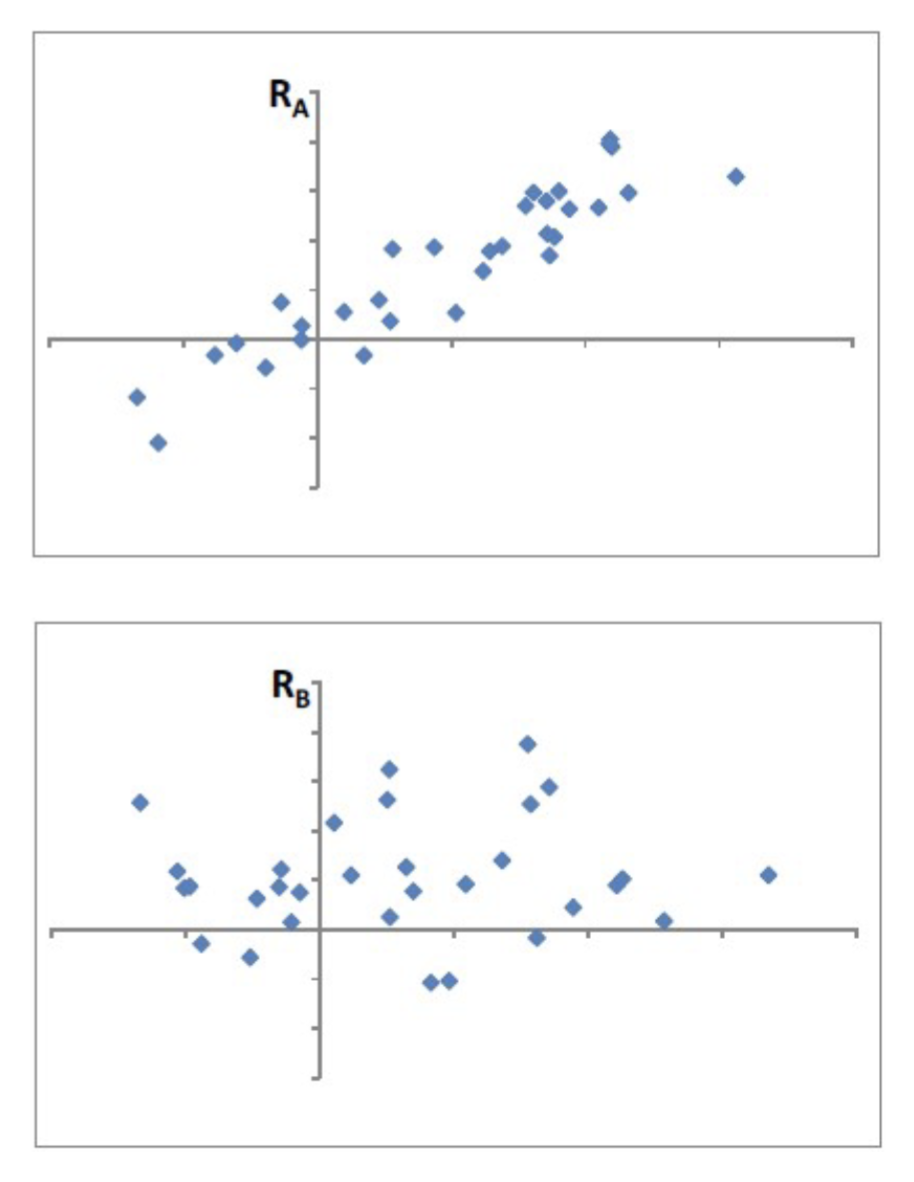
\includegraphics[scale=0.20]{20.png}
     \caption{Sammenhæng mellem årlige afkast for givne virksomheder og markedsporteføljen}
     \label{Figur 2}
\end{figure} 

Af afsnittet om estimation af beta værdier vha. markedsindekset følger det, at virksomhed A har en højere betaværdi, og dermed et højere afkastkrav og dermed en højere egenkapitalsomkostning.

\subsection{Aktiers fundamentale værdi}
En akties fundamentale værdi kan estimeres ved en såkaldt \textbf{dividend discount model (DDM)}, der estimerer den fundamentale værdi af en aktie som nutidsværdien af de fremtidige dividender:

\begin{equation}
     V_0 = \frac{D_1}{(1 + k)} + \frac{D_2}{(1 + k)^2} + \frac{D_3}{(1 + k)^3} + \ldots
\end{equation}

hvor diskonteringsraten $k$ afspejler \textbf{afkastkravet} (fundet fra CAPM!) til aktien, givet dens risiko. Hvis divendeudbetalinger er konstante ud i al fremtidig er værdien: 

\begin{equation}
        V_0 = \frac{D_1}{k}
\end{equation}

Mens nutidsværdien er givet ved nedenstående, hvis der er en årlig vækst på $i$ i udbyttebetalingerne: 

\begin{equation}
        V_0 = \frac{D_1}{k - g}
\end{equation}

Hvis $V_0 < \text{kurs}$ er aktien overvurderet og bør sælges, mens $V_0 > \text{kurs}$ indikerer at aktien er undervurderet og bør købes. Udfordringen ved modellen er dog, at den kræver, at man kender alle fremtidige dividende udbetalinger. Betragt eksempel 10, der viser en gennemgang heraf. 

\begin{tcolorbox}[breakable, colback=red!5!white, colframe=red!50!black, title= Eksempel 10: Beregning af fundamental værdi for et værdipapir]
Betragt en aktie, der udbetales 54 kr. pr. aktie i det kommende 5 år, hvorefter dividenderne vokser med 1,5 pct. om året. Diskonteringsrenten er 7 pct. Indledningvis bestemmes nutidsværdien af de indiviudelle betalinger de første 5 år: 

\begin{equation*}
    NPV_{1} = \frac{54}{(1+0,07)^1} + \frac{54}{(1+0,07)^2} + \frac{54}{(1+0,07)^3} + \frac{54}{(1+0,07)^4} + \frac{54}{(1+0,07)^5} = 221,41
\end{equation*}

Herefter bestemmes nutidsværdien af den voksende perpuitet: 

\begin{equation*}
    NPV_{2} = \frac{54 \cdot (1+0,015)}{0,07 - 0,015} = 996,54
\end{equation*}

Hvilket skal tilbagediskonteres 5 år: 

\begin{equation*}
    NPV_{3} = \frac{996,54}{(1+0,07)^5} = 710,52
\end{equation*}

Hvorfor den samlede nutidsværdi er givet ved: 

\begin{equation*}
    NPV_1 + NPV_3 = 221,41 + 710,52 = 931,93
\end{equation*}
\end{tcolorbox}

Hvis en virksomhed ikke betaler udbytte erstattes DDM med \textbf{'free cash flow to equity'}, der erstatter hvor meget virksomheden potentielt kunne have udbetalt i udbytte. 

\begin{equation}
    V_0 = \frac{FCFE_1}{(1 + k)} + \frac{FCFE_2}{(1 + k)^2} + \frac{FCFE_3}{(1 + k)^3} + \ldots
\end{equation}

hvor $FCFE = \text{Resultat} + \text{Afskrivninger} - (\text{Afdrag på gæld} - \text{optagelse af ny gæld}) -\text{nettoinvesteringer}$

\newpage

Afsluttende kan \textbf{'free cash flow to firm (FCFF)'} er et eksempel på en DCF-metode som tager højde for markedsværdien af hele virksomheden. FCFF bestemmes altså som nutidsværdien af de fremtidige cash flows, som virksomheden potentielt kan bruge til at \textit{udbetale dividender og servicere gæld}.

\begin{equation*}
        V_0 = \frac{FCFF_1}{(1 + k)} + \frac{FCFF_2}{(1 + k)^2} + \frac{FCFF_3}{(1 + k)^3} + \ldots
\end{equation*}

Hvor FCFF er bestemt som: Resultat per aktie + afskrivninger + rentebetalinger (efter skat) - investeringer - udbytte til præferenceaktier (preffered stocks).

\subsection{Efficiente markeder}
Et marked siges at være informationsmæssigt \textbf{efficient}, hvis
priserne på et givet tidspunkt reflekterer al tilgængelig information. En illustration af et efficient marked er vist nedenfor, hvor markedsprisen stiger så snart der er kommet ny information, der har positiv indflydelse på aktiens situation: 

\begin{figure}[h]
     \centering
     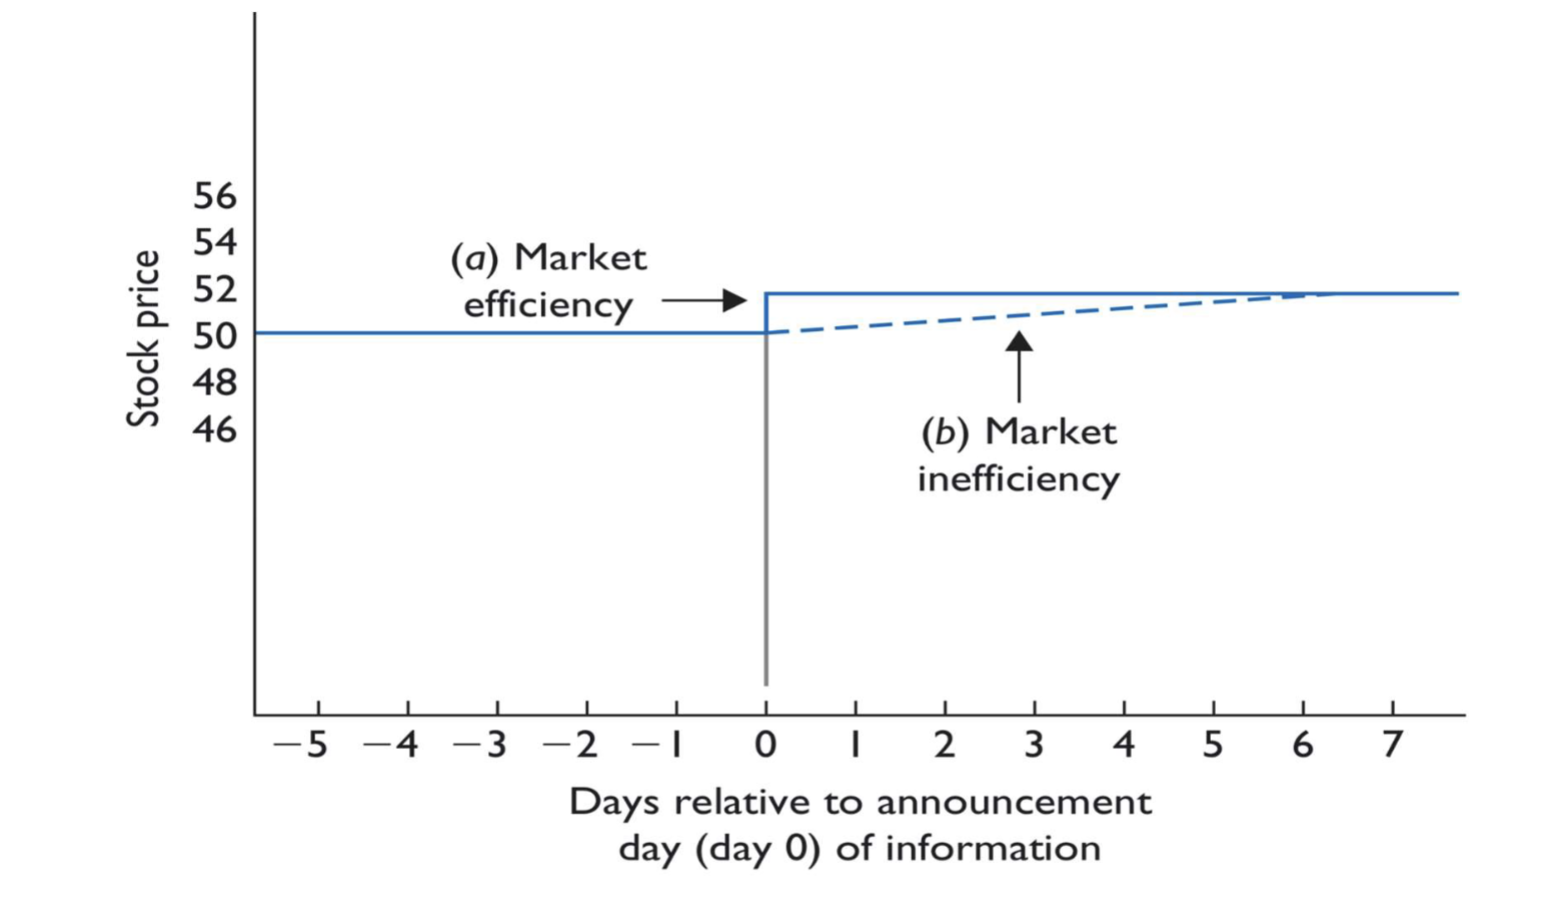
\includegraphics[scale=0.35]{21.png}
     \caption{Visualisering af efficiente markeder}
     \label{Figur 2}
\end{figure} 

\textbf{Implikationerne af et effektivt marked} er: 
\begin{itemize}
    \item På et efficient marked har ethvert værdipapir på ethvert givet tidspunkt et forventet afkast, som er i overensstemmelse med dets risiko (\(\beta\)).
    \item Aktiekurser tilpasser sig øjeblikkeligt til nyt ligevægtsniveau, når ny information fremkommer.
    \item Aktiekurser reflekterer altid al tilgængelig information $\rightarrow$ ikke muligt at systematisk "slå markedet" ved selv at indsamle og anvende information (eller ved at betale andre for det).
    \item En aktiv investeringsstrategi (hyppige handler som reaktion på ny
information) giver  ikke højere forventet afkast, men øger omkostninger i form af gebyrer og tid anvendt til
informationsindsamling.
\item \textit{Passiv} investeringsstrategi (sammensæt bred portefølje og behold den) bliver  mere attraktiv
\item \textbf{Den eneste måde at øge sit forventede afkast på er ved at påtage sig mere risiko}
\end{itemize}

\textbf{Følgende forudsætninger} skal være opfyldt for at et marked kan siges at være efficient: 

    \begin{enumerate}
        \item Et stort antal pristagende investorer, som analyserer, værdiansætter og handler aktiver med henblik på at få størst muligt forventet afkast, givet risikoen
        \item Information bliver omkostningsfrit stillet til rådighed for alle investorer på samme tid
        \item Alternativt: Hvis alle ikke har samme information men at der er mulighed for arbitrage vil selv - arbitrage - investorer få priserne til at justere mod ligevægt.
    \end{enumerate}

Det betyder imidlertid ikke, at  at aktiekursen på ethvert tidspunkt
svarer præcist til aktiens fundamentale værdi, men at den
repræsenterer markedets bedste bud på denne ud fra den tilgængelige information.

\vspace{10 pt}

\textbf{Kritikken af de efficiente markeder er}, at; 
\begin{itemize}
    \item Det ikke er omkostningsfrit at samle og bearbejde information
    \begin{itemize}
        \item Ex: Professionelle investorer kunne have et andet arbejde $\rightarrow$ alternativomk. ved tid brugt på at læse årsregnskaber osv. $\rightarrow$ kræver kompensation for at gøre det
    \end{itemize}
    \item Hvis markederne var efficiente, så der ingen gevinst var ved at indsamle information:
    \begin{itemize}
        \item Ingen ville afholde omkostningen ved at indsamle information
        \item Markedspriserne ville ikke afspejle den tilgængelige information
    \end{itemize}
    \item Implikationer:
    \begin{itemize}
        \item Markederne kan ikke være fuldkommen efficiente
        \item Der må nødvendigvis være en (lille) gevinst ved at samle og bearbejde information
        \item Det afgørende er hvor lang tid det tager at justere og hvor meget "over"-normal profit der kan laves i justeringsperioden.
    \end{itemize}
\end{itemize}

Det følger heraf, at der findes 3 forskellige grader af efficiente markeder, der er defineret som: 

\begin{enumerate}
    \item \textcolor{red}{Svag} EMH: nuværende markedspriser reflekterer alt generelt tilgængeligt markedsinformation (historiske priser).
    \item \textcolor{red}{Halvstærk} EMH: nuværende markedspriser reflekterer al offentligt tilgængeligt information
    \item \textcolor{red}{Stærk} EMH: nuværende markedspriser reflekterer al information (både offentlig og privat)
\end{enumerate}

\subsection{Svag EMH}
Den svage EMH implicerer således, at historiske prisdata ikke kan bruges til at forudsige fremtidige prisændringer. Der er generelt solidt empirisk belæg for den svage EMH, selvom man godt kan opnå små prisgevinster ved at handle på tværs af markeder, hvor information bliver \textit{spredt} med forskellig tid. Her vil det dog i praksis ofte være sådan, at transkationsomkostningerne er højere end den potentielle gevinst ved en sådan strategi. Finansielle markeder er altså \textbf{økonomisk efficiente}, snarere end \textbf{statistisk efficiente}.


\subsection{Semistærk EMH}
Den semistærke EMH forudsiger, at de nuværende markedspriser reflekterer al tilgængelig information, hvorfor aktiekurser tilpasser sig øjeblikkeligt, når ny information bliver offentligt tilgængeligt. Man kan teste for EMH ved at foretage eventstudier og undersøge, hvordan aktiekursen opfører sig i dagene op til annonceringen. Den semistærke EMH siges at holde, hvis ny information fører til spring i aktiekurser og der ikke er nogen systematisk ændring efter perioden (f.eks. en varig stigning). Omvendt siges det ikke at holde, hvis ny  information fører til systematiske kursændringer i perioden efter annoncering. For at teste den semistærke EMH skal man (1) estimere aktiens overnormale afkast som forskellen mellem det faktiske afkast, $R_{it}$ og det forventede afkast $E[R_{it}]$. Altså; 

\begin{equation}
    AR_{it} = R_{it} - E[R_{it}]
\end{equation}

Hvorefter det kumulerende overnormale afkast for perioden bestemmes som: 

\begin{equation}
    CAR_{it} = \sum_{s=0}^{t} AR_{is}
\end{equation}

Ved at plotte en serie af de overnormale afkast kan man se, hvor hurtigt markedet reagerer på ny information. Nedenfor vil der f.eks. ikke være tale om den semistærke EMH, idet de virksomheder, der falder indledningsvist bliver ved med at falde og dem, der stiger indledningsvist bliver ved med at stige. 

\begin{figure}[h]
     \centering
     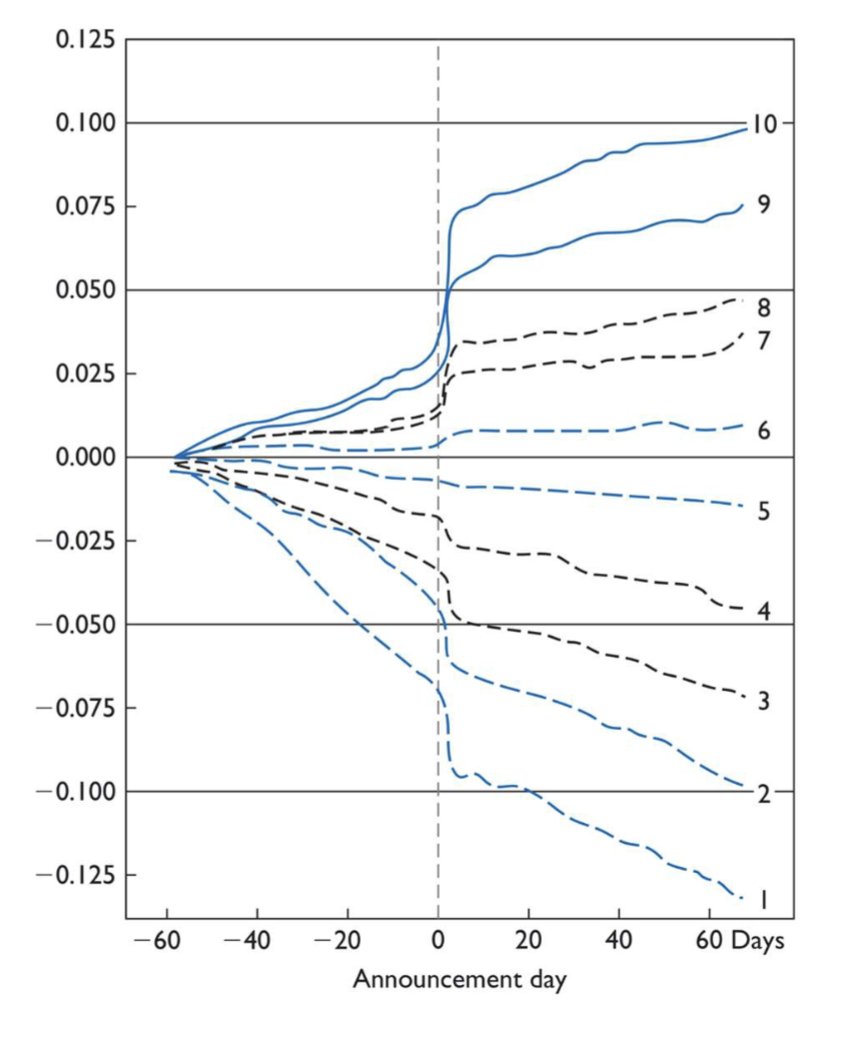
\includegraphics[scale=0.4]{22.png}
     \caption{Eksempel af CAR hvor semistærk EMH ikke er opfyldt}
     \label{Figur 2}
\end{figure} 

\subsection{Stærk EMH}
Den stærke EMH beskriver, at nuværende markedspriser reflekterer al information - både offentligt tilgængelig og privat information. Altså; aktiekurser skal tilpasse sig med det samme, når ny information bliver tilgængelig for offentligheden eller for private aktører. Heraf følger, at man selv med insiderviden ikke kan slå markedet. Den stærke EMH kan virke restriktiv, men det gælder, at andre insider kan handle før dig og at flashtrading generelt kan betyde, at selv mikrosekunder kan gøre en stor forskel, når man handler aktier i en periode, hvor der \textit{sker meget på markedet}. 



\newpage
\section{BMT}
\subsection{BMT 1 — virksomhedens Formål}
\textbf{Friedman Doktrinet} tilsiger, at virksomhedens \textit{eneste} rolle er at maksimere sit overskud, så gældende love overholdes, og virksomheden opererer i et frit marked. Den underliggende præmis er her, at \textbf{frie markeder maksimerer samfundsvelfærden} (positivt argument). Det skyldes, at konkurrence vil drive virksomheder til at være efficiente og
innovative, mens prissystemet vil gøre det muligt at koordinere
millioner af virksomheder og milliarder af ansatte. Til grund herfor ligger desuden, at direktører og ledere er agenter for virksomhedens
ejere (normativt). Der er dog følgende antagelser, der skal være opfyldt for at præmissen gælder; 

\begin{itemize}
    \item  Fri konkurrence
    \item Fravær af monopolister ('monopolistic power')
    \item Fravær af collusion
    \item Symmetrisk information
    \item Prisfastsættelse af eksternaliteter
    \item Stærke regeringer og supra nationale institutioner
\end{itemize}

\textbf{Friedman Doktrinet har dog udlevet sig selv}, fordi; 

\begin{itemize}
    \item Skatter og afgifter får ikke virksomheder til at internalisere eksternaliteter: eksternaliteter er ikke prisfastsat korrekt $\rightarrow$ miljøkonsekvenser af virksomhedsdrift
    \item Der eksisterer udbredt markedspower (Google)
    \item Der er ikke symmetrisk information, globale virksomheder har mere information end regeringer og andre.
    \item Virkeligheden har ændret sig fra koldkrigsfrygt, verden er ikke enten kommunistisk eller fri. CSR/ESG er IKKE lig med Kommunisme.
    \item Virksomhedsledere er ikke juridisk bundet til KUN at maksimere aktionærværdi. Fiduciary principle.
    \item $\rightarrow$ I dag er der mange formålsdrevne virksomheder der er drevet af bredere målsætning end profitmaksimering som f.eks. social ansvarlighed. Ofte er det drevet af visionære ledere der kan se business muligheder.
\end{itemize}

\subsection{BMT 2 — sustainability regnskab}
Det finansielle regnskab angiver den økonomiske situation som shareholders for ud af en  (f.eks. drift, finansiering, investering) virksomhed (defineret som en juridisk enhed), der ejer aktiver og indgår kontrakter. Sustainability regnskabet tager derimod udgangspunkt i hvordan virksomheden påvirker alle stakeholders, herunder: ledelse, investorerer, ansatte, nærområdet, miljøet, ligestilling, osv. Billedet nedenfor viser de forskellige \textit{scopes}, der kan medtages i sustainability regnskabet: 

\newpage
\begin{figure}[h]
     \centering
     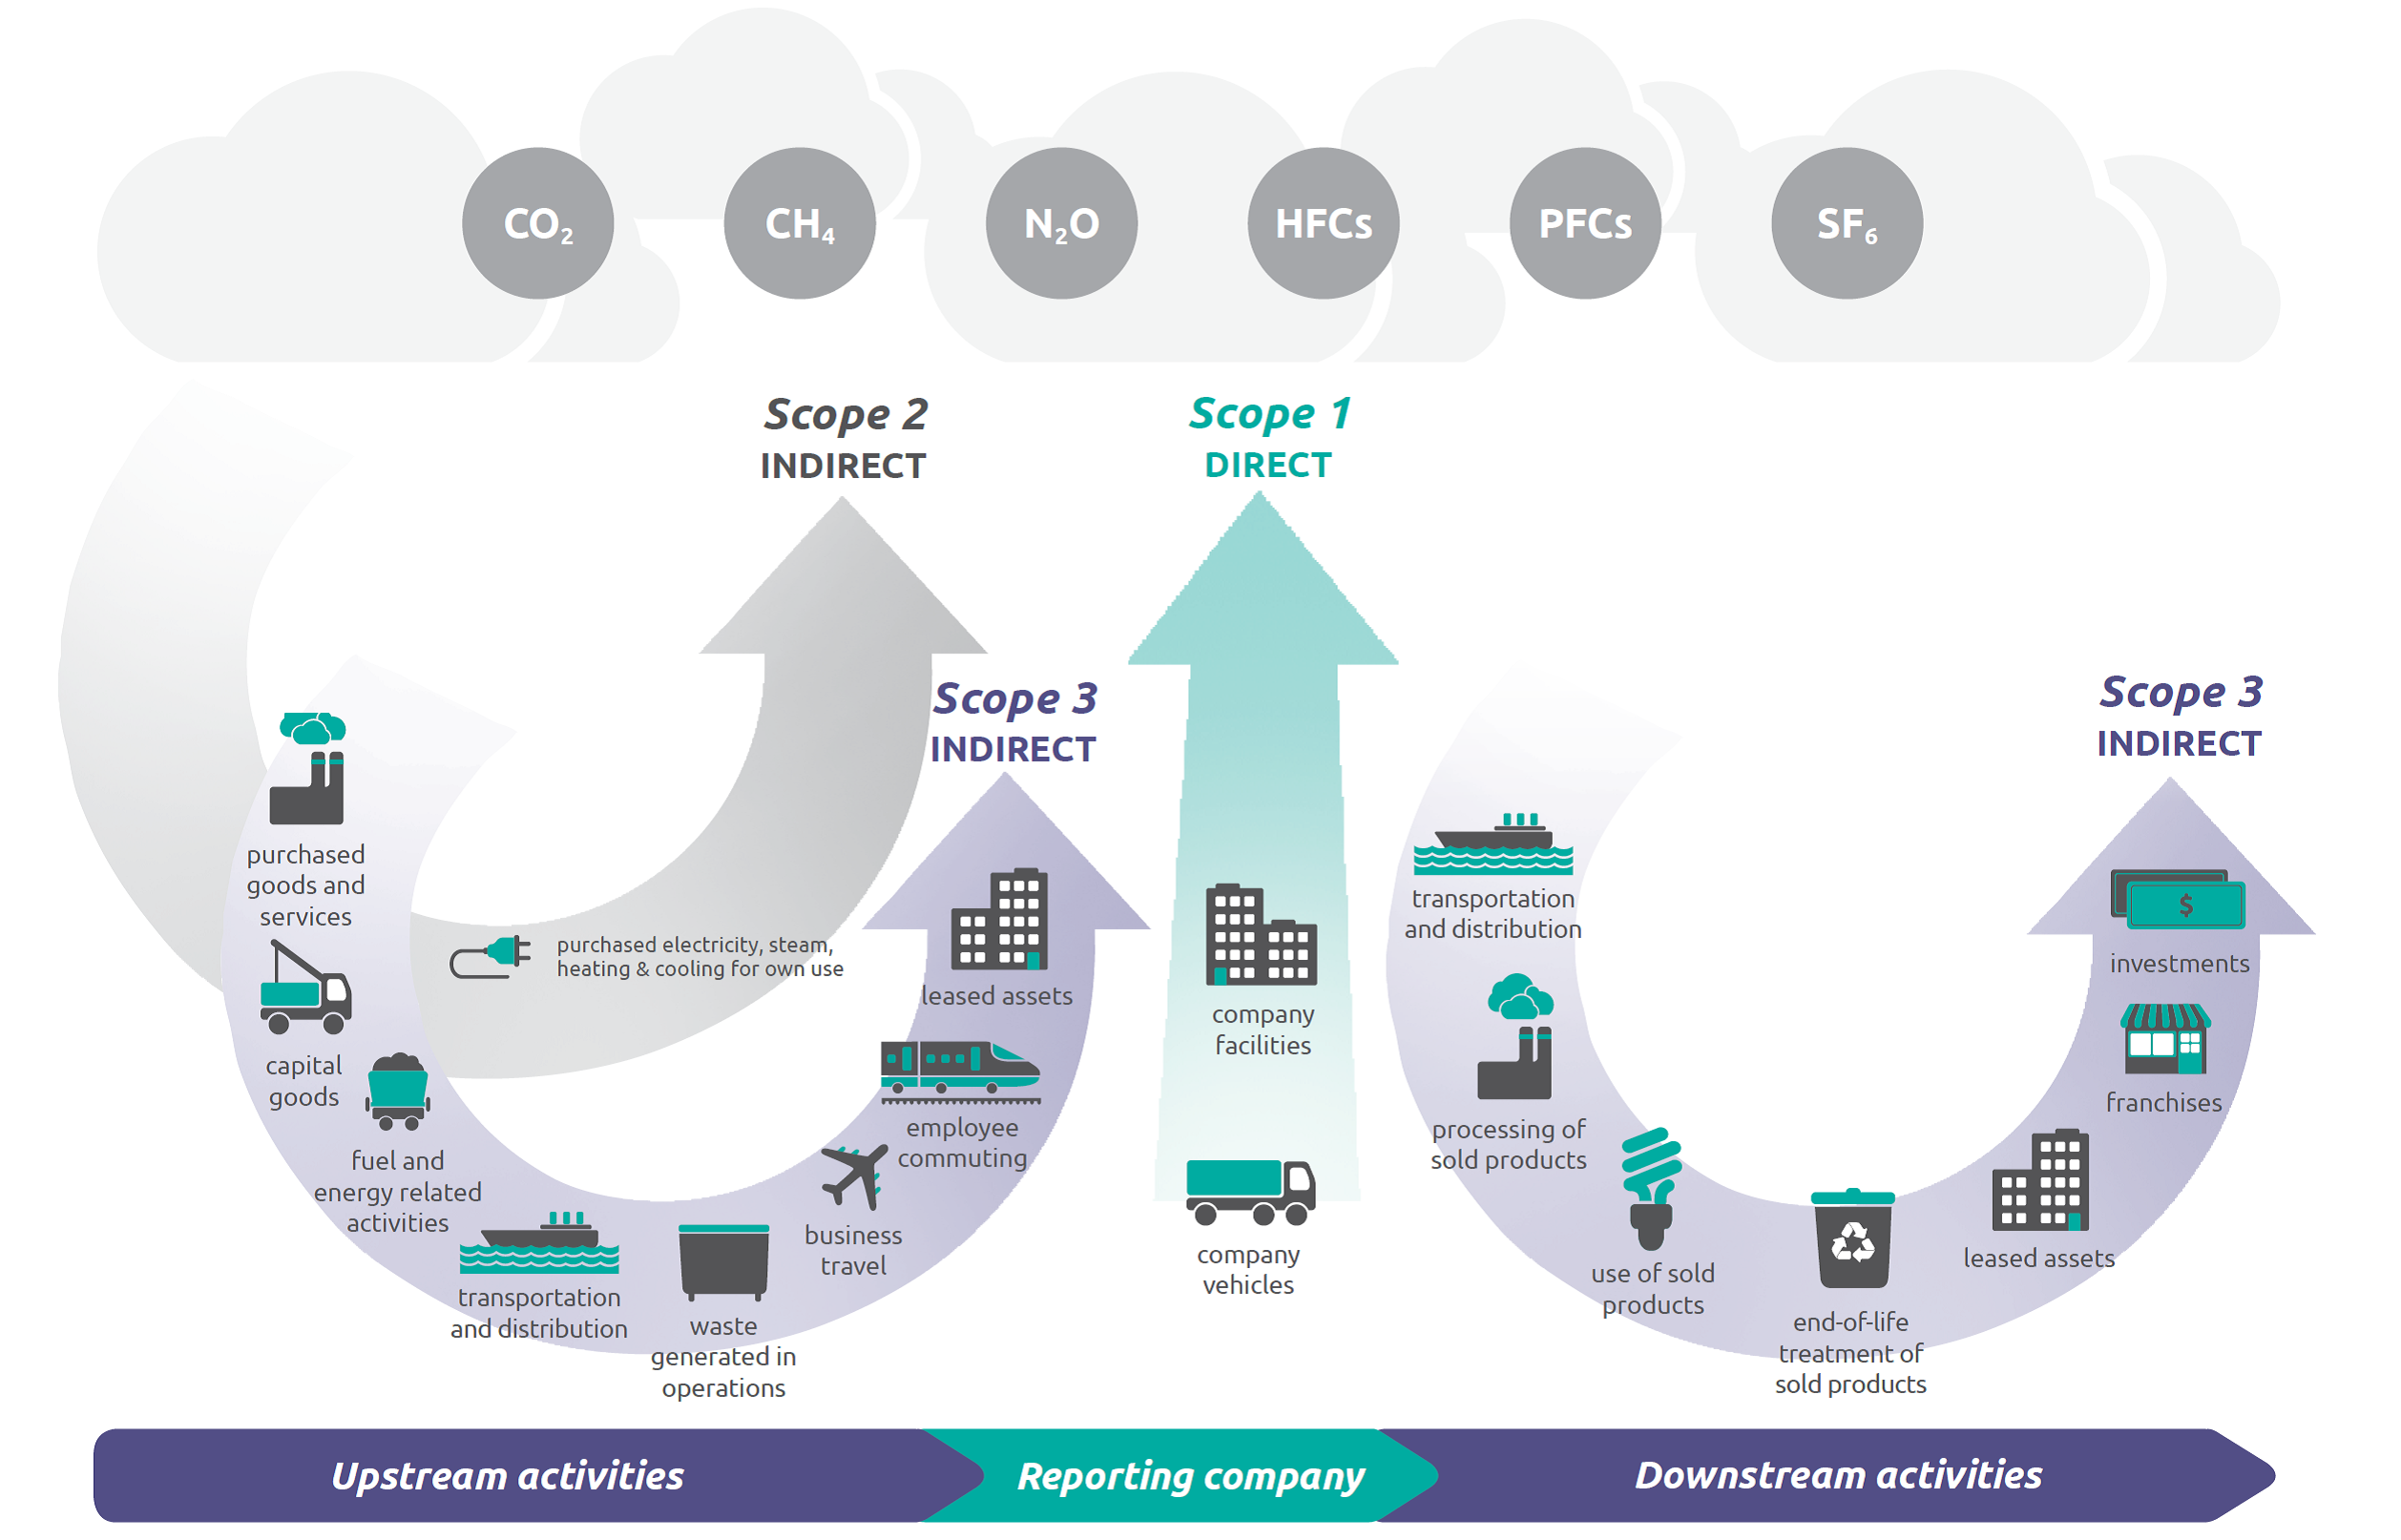
\includegraphics[scale=0.10]{23.png}
     \caption{Oversigt over forskellige ESG \textit{scopes}}
     \label{Figur 2}
\end{figure} 

Det skal nævnes, at der \textbf{ikke} er generel evidens for, at sustainability strategier er profitable, mens det dog kan tænkes, at investorerer, ansatte og forbrugere vil affinde sig med hhv. lavere afkast, lavere løn og højere priser, hvis det kan være godt for f.eks. miljøet. Det nedenstående \textit{flow} viser, hvordan ESG/purpose kan operationaliseres: 

\begin{figure}[h]
     \centering
     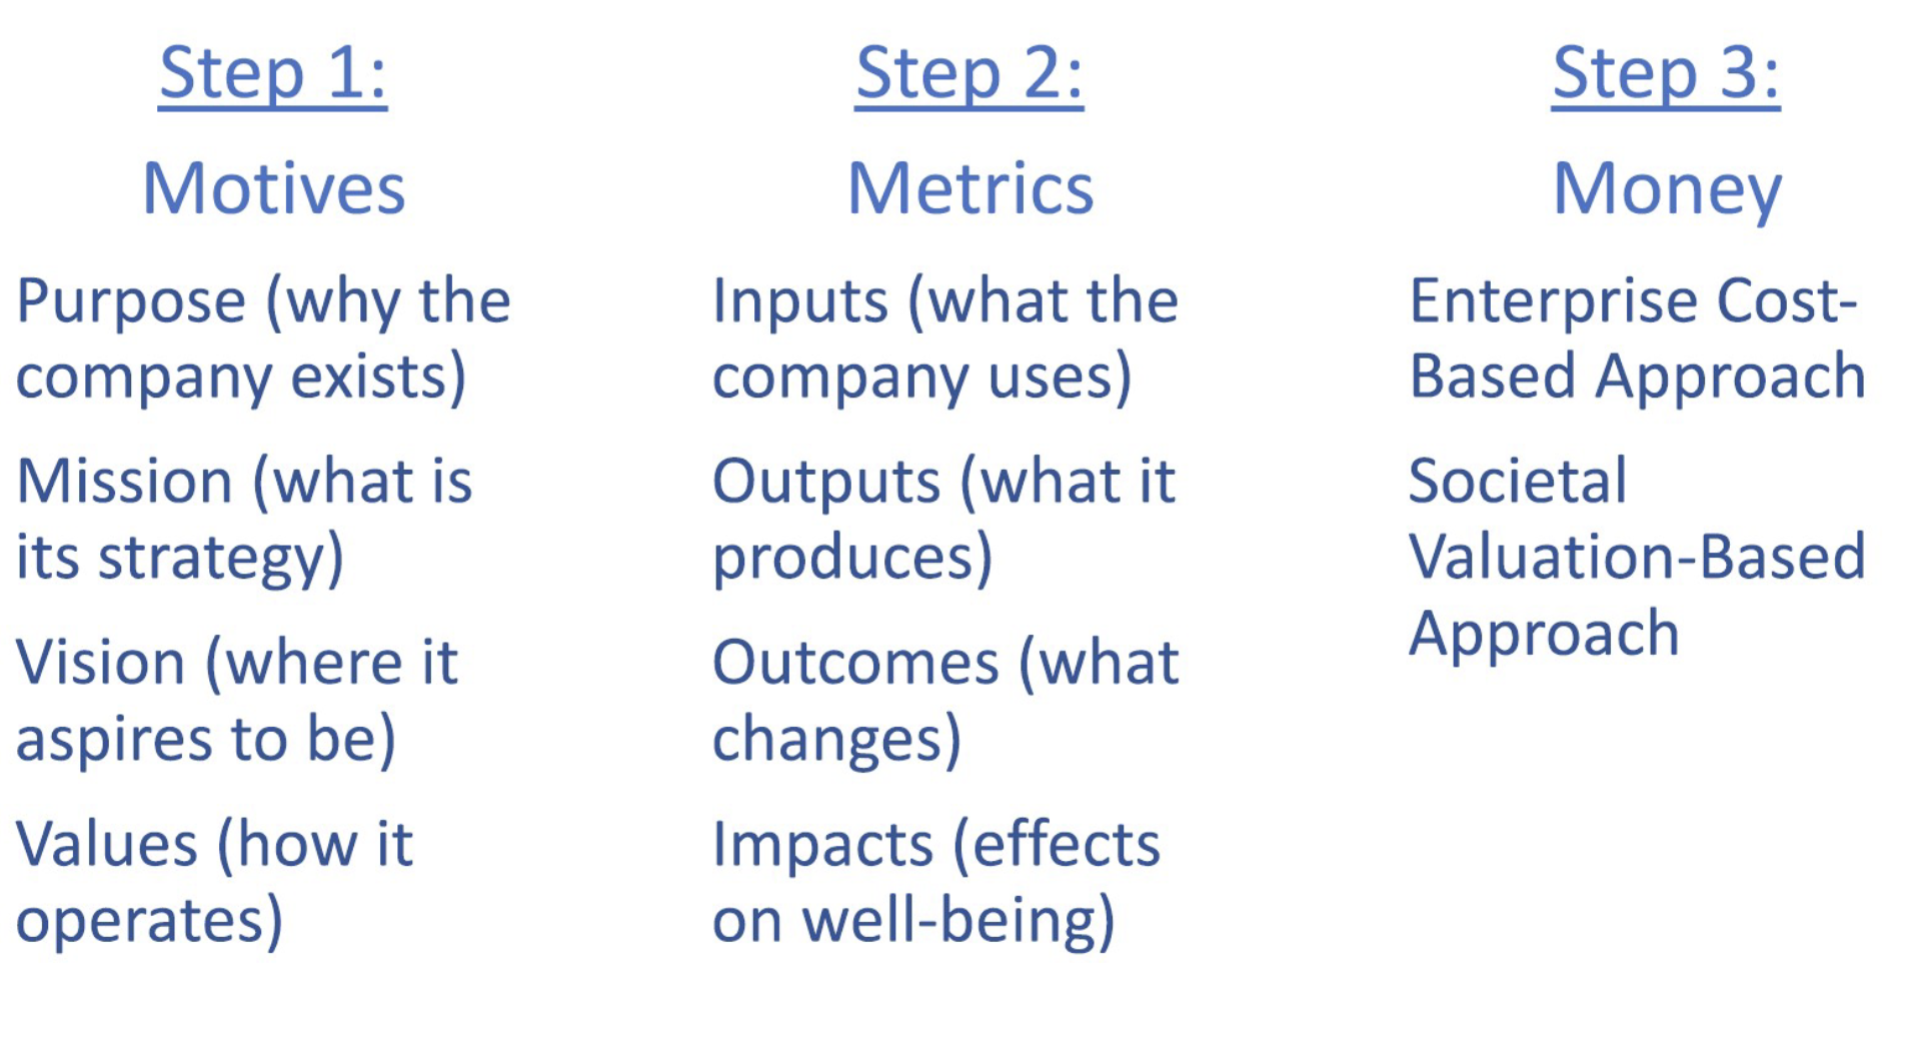
\includegraphics[scale=0.25]{24.png}
     \caption{Operationalisering af ESG mål}
     \label{Figur 2}
\end{figure} 

For at estimere \textbf{stakeholderværdien} som en virksomhed skaber, kan nedenstående tabel desuden være nyttig: 

\begin{figure}[h]
     \centering
     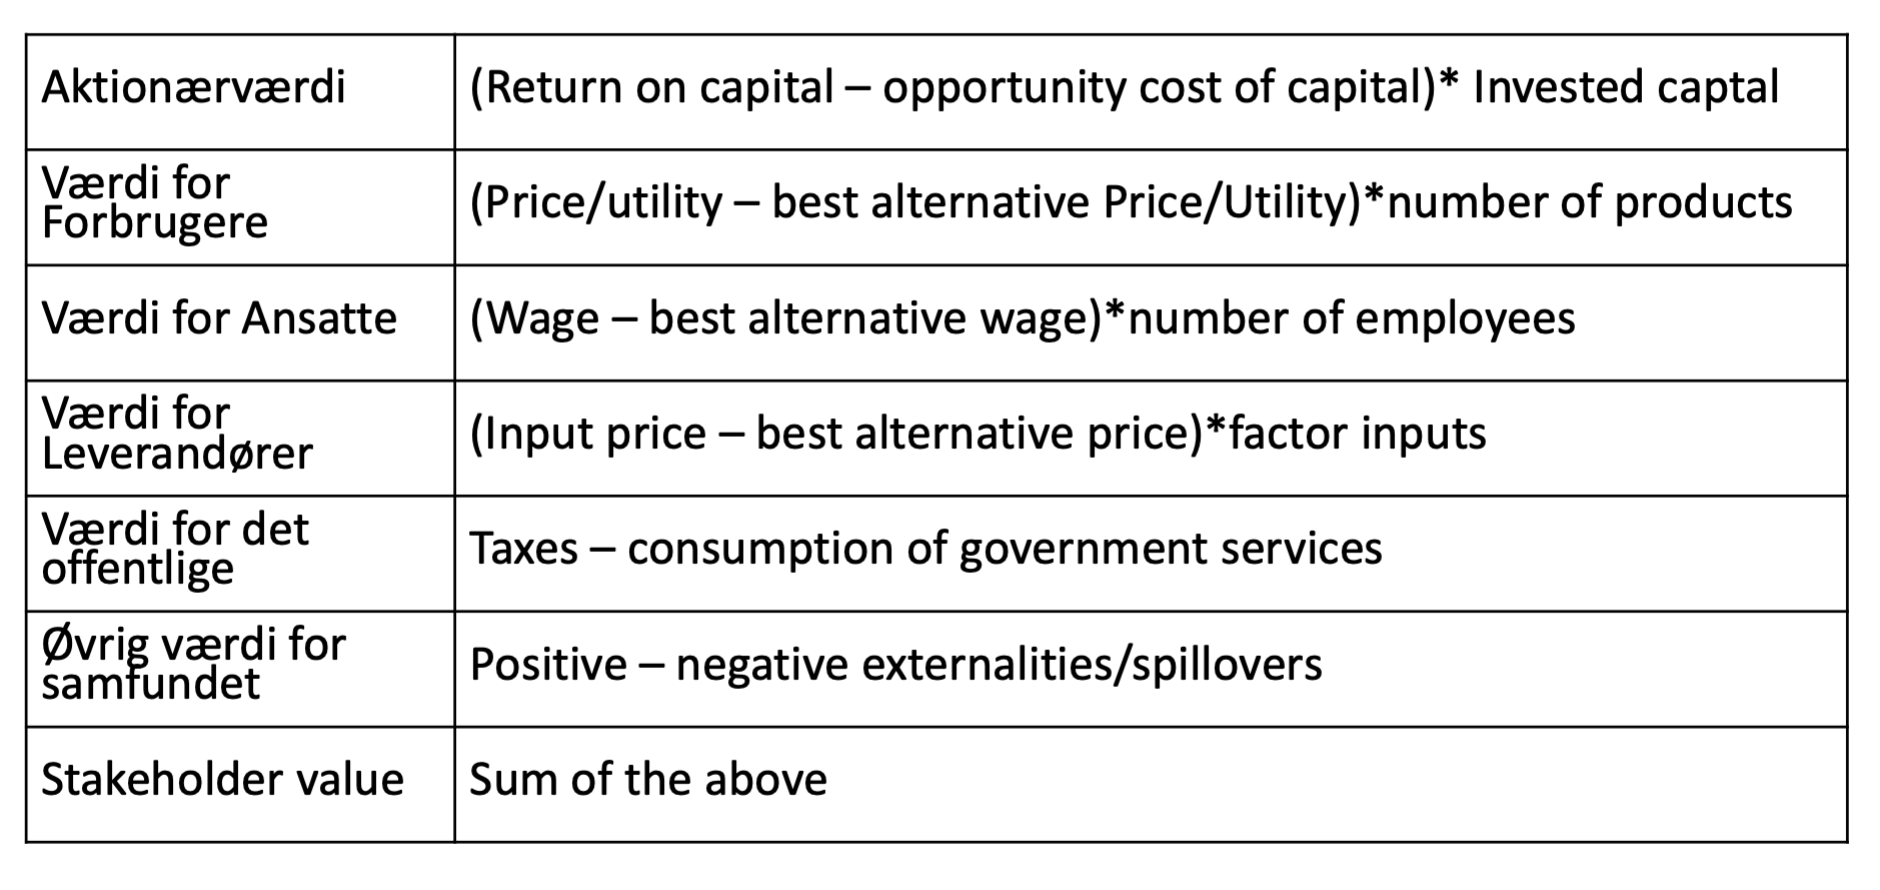
\includegraphics[scale=0.25]{25.png}
     \caption{Fra shareholder- til stakeholderværdi}
     \label{Figur 2}
\end{figure} 

Et rating bureau kan desuden give de enkelte virksomheder en rating på baggrund af, i hvor høj grad de lever op til deres sociale forpligtelser (AAA er det højeste). Se nedenfor: 

\newpage

\begin{figure}[h]
     \centering
     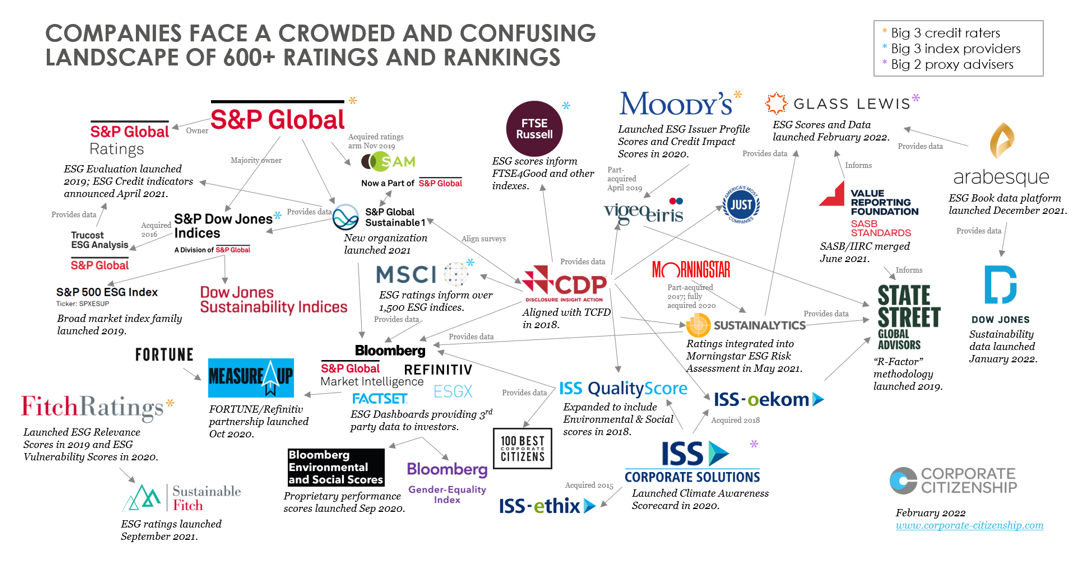
\includegraphics[scale=0.35]{26.png}
     \caption{Forskellige ESG rating udbydere}
     \label{Figur 2}
\end{figure} 

\subsection{BMT 3 — ejerskab}
Der er følgende ejerskabsformer, der gennemgås i det følgende: 

\begin{itemize}
    \item Ejerleder
    \item Flere direkte ejere 
    \item Familie ejet
    \item Kapitalfonde
    \item Hedgefonde
    \item Børsnoterede
    \item Fondsejede
\end{itemize}

Fordele og ulemper ved \textbf{ejerledere} er:

\begin{table}[h!]
\centering
\begin{tabular}{|m{5cm}|m{5cm}|}
\hline
\textbf{\textcolor{red}{Fordele}} & \textbf{\textcolor{red}{Ulemper}} \\
\hline
\textcolor{olive}{Entrepreneur er ildsjæle og gode til at drive virksomheden fremad.} & Mangler Checks and Balance \\
\hline
\textcolor{olive}{Effektiv ledelse, der hurtigt kan tage beslutninger} & Uprofessionel selskabsstyring/corporate governance. \\
\hline
 & Svage bestyrelser \\
\hline
 & Kvalitet i Human resource. \\
\hline
 & Virksomhedens vækstpotentiale afhænger af ejerlederens kapacitet \\
\hline
 & Key personal risk (virksomheden er sårbar). \\
\hline
\end{tabular}
\caption{Fordele og ulemper ved ejerledede virksomheder}
\end{table}

Fordele og ulemper ved \textbf{børsnoterede virksomheder} er:

\begin{table}[h!]
\centering
\begin{tabular}{|m{5cm}|m{5cm}|}
\hline
\centering \textbf{\textcolor{red}{Fordele}} & \centering \textbf{\textcolor{red}{Ulemper}} \tabularnewline
\hline
\textcolor{olive}{Kapitaltilgang} & Svært at dreje skuden over natten. \tabularnewline
\hline
\textcolor{olive}{Selskabsledelse} & Styret af kvartalsregnskaber og aktionærværdien \tabularnewline
\hline
\textcolor{olive}{Transparans} & Topledelses aflønning: Niveau og incitamentsstrukturer. \tabularnewline
\hline
& Besværligt... ? (Hvis man var noget andet før). \tabularnewline
\hline
\end{tabular}
\caption{Fordele og ulemper ved børsnotere virksomheder}
\end{table}

\newpage
Fordele og ulemper ved \textbf{familieejede virksomheder} er:

\begin{table}[h!]
\centering
\begin{tabular}{|m{5cm}|m{5cm}|}
\hline
\centering \textbf{\textcolor{red}{Fordele}} & \centering \textbf{\textcolor{red}{Ulemper}} \tabularnewline
\hline
\textcolor{olive}{Værdibaserede} & Mangler Checks and Balance \tabularnewline
\hline
\textcolor{olive}{Langsigtede} & Uprofessionel selskabsstyring/corporate governance. \tabularnewline
\hline
\textcolor{olive}{Stewardship} & Svage bestyrelser \tabularnewline
\hline
\textcolor{olive}{Loyalitet} & Nepotisme \tabularnewline
\hline
\textcolor{olive}{Effektiv ledelse, der hurtigt kan tage beslutninger} & Er næste generation god nok? Transition gennem generationer. \tabularnewline
\hline
\textcolor{olive}{Stærkt netværk} & \tabularnewline
\hline
\end{tabular}
\caption{Fordele og ulemper ved familieejede virksomheder}
\end{table}

Fordele og ulemper ved \textbf{kapitalfondsejerskab} er:

\begin{table}[h!]
\centering
\begin{tabular}{|m{6cm}|m{6cm}|}
\hline
\centering \textbf{\textcolor{red}{Fordele}} & \centering \textbf{\textcolor{red}{Ulemper}} \tabularnewline
\hline
\textcolor{olive}{Vækst fokuseret} & Horisont? 4-6 år så skal den sælges. \tabularnewline
\hline
\textcolor{olive}{Betaler en god pris} & Tænker kun på aktionærværdien. \tabularnewline
\hline
\textcolor{olive}{Klar strategi} & Ansattes velfærd? \tabularnewline
\hline
\textcolor{olive}{Ansætter gode ledere med de rigtige incitamenter.} & Splitter virksomheder op hvis det giver værdi. \tabularnewline
\hline
\textcolor{olive}{Hurtig og effektiv selskabsledelse.} & Skat? Ofte snedige skattekonstruktioner for partnere og virksomheder. \tabularnewline
\hline
\textcolor{olive}{Stærkt netværk og stor erfaring.} & \tabularnewline
\hline
\end{tabular}
\caption{Fordele og ulemper ved kapitalfondsejerskab}
\end{table}

Fordele og ulemper ved \textbf{fondsejerskab} er:

\begin{table}[h!]
\centering
\begin{tabular}{|m{6cm}|m{6cm}|}
\hline
\centering \textbf{\textcolor{red}{Fordele}} & \centering \textbf{\textcolor{red}{Ulemper}} \tabularnewline
\hline
\textcolor{olive}{Langsigtet drift} & Empower daglig ledelse, svage ejere. \tabularnewline
\hline
\textcolor{olive}{Stewardship} & Bestyrelsens rolle? \tabularnewline
\hline
\textcolor{olive}{Skal ikke tage (meget) hensyn til analytikere og potentielle overtagelser etc} & Kan skibet vendes hurtigt hvis det kræves? \tabularnewline
\hline
\textcolor{olive}{Mange fonde har en filantropisk side (Novo Nordisk, Carlsberg, Rockwool, Villum, etc)} & Charter kan være restriktivt for nye initiativer. \tabularnewline
\hline
\end{tabular}
\caption{Fordele og ulemper ved fondsejerskab}
\end{table}

Der er desuden 3 grundlæggende \textbf{agency problemer}: 
\begin{itemize}
    \item Owner-manager $\rightarrow$ ejere vil have højt afkast, lav risiko og stort overskud, mens lederne vil have høj løn, anerkendelse, osv. 
    \item Minority-majority owners $\rightarrow$ majority investorer vil have langsigtet profit, lav risko og kontrol, mens miniority owners vil have kortsigtet profit
    \item Shareholder-stakeholder $\rightarrow$ shareholders vil have profit og vækst i virksomheden, mens stakeholderne vil have billige produkter, høje lønninger, ESG osv.
\end{itemize}

Til spørgsmålet om, hvorvidt familiejede virksomheder en \textit{en force of good}, kan nedenstående billede betragtes: 

\begin{figure}[h]
     \centering
     
\includegraphics[scale=0.45]{27.png}
     \caption{Vurdering af familieejede virksomheder i ESG-kontekst}
     \label{Figur 2}
\end{figure} 

\subsection{BMT 4 — virksomhedsledelse}
De forskellige trends indenfor \textit{corporate governance} har været: 

\begin{figure}[h]
     \centering
     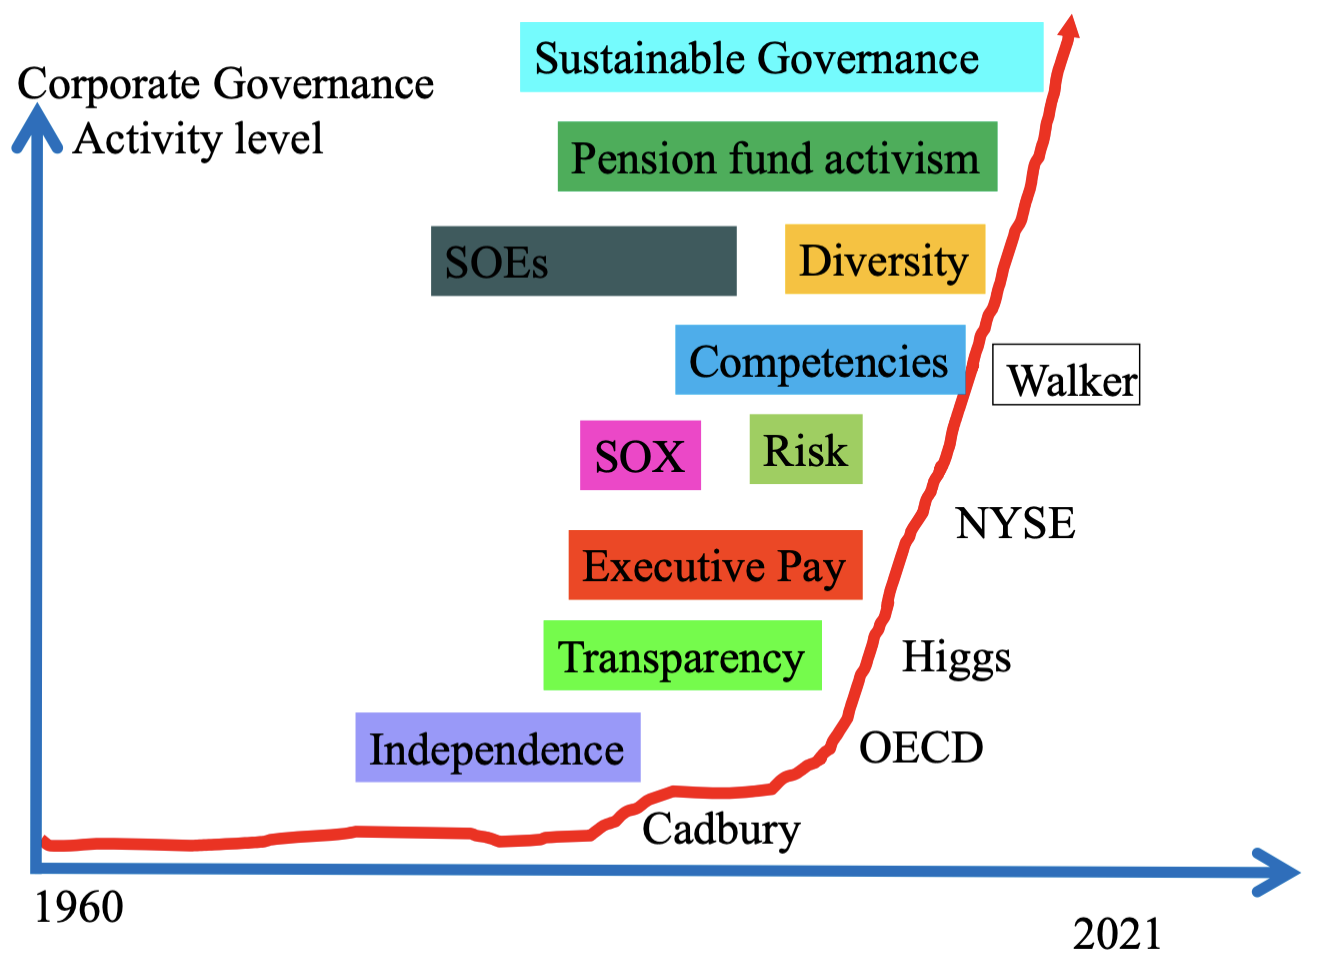
\includegraphics[scale=0.45]{28.png}
     \caption{Udvikling i \textit{corporate governance}}
     \label{Figur 2}
\end{figure} 

Mens de overordnede principper i \textit{corporate governance} er: 

\begin{itemize}
    \item Checks and balances – sharing of power
    \item Boards (directors) vs Executives (direktion)
    \item Transparency – information \& openness
    \item Value creation – for shareholders and society
    \item Fairness – equality
    \item Duty of loyalty
    \item Duty of care
    \item Incentives – self interest
    \item Accountability – being held responsible
    \item Stewardship – responsible long-term ownership
    \item Agency – acting on behalf of others
\end{itemize}

Mens \textbf{værdibaseret ledelse} er defineret som når; \textit{when decision-making and governance in a firm mirror the personal values of the individuals in charge. (Bennedsen and Fan 2014)}. Altså; 

\begin{itemize}
    \item Values are used as guidelines for decision-making in general and in particular in unprecedented situations (in contrast to experience based or KPI based decision-making). Think Covid19 and Russia's Invasion of Ukraine.
    \item Values provide an identity for the firm and its stakeholders, and generate a formal or informal code of conduct.
    \item $\rightarrow$ Clear values reduce coordination costs by permitting less monitoring and leading to higher effort.
\end{itemize}


\subsection{BMT 5 — offentlige anlægsinvesteringer}
Offentlige anlægsinvesteringer følger grundlæggende de samme \textit{mekanismer} som private anlægsinvesteringer, beskrevet i afsnit \textbf{3}. Altså; gennemfør den investering, der har den største NPV (såfremt denne er positiv). Den store forskel er dog, at offentlige anlægsinvesteringer monetariserer eksternaliteter, der (ofte) ikke medregnes i traditionelle investeringskalkuler. Desuden er der indenfor offentlige anlægsinvesteringer blevet fastsat en bindende kalkulationsrente, det betyder, at den offentlige kalkulationsrente: 

\begin{itemize}
    \item Er politisk fastsat under skelen til den forventede langsigtede realrente. 
    \item Er blevet sat ned de sidste par år for at få gang I grøn omstilling!
    \item Ikke afhænger af den øjeblikkelige låneomkostning.
    \item Ikke har nogen direkte sammenhæng med alternativomkostninger. 
    \item Risikopræmien ikke afhænger af projektet. 
\end{itemize}

Den samfundsmæssige kalkulationsrente er: 

\begin{itemize}
    \item 0 - 35 år: 3,5 pct. 
    \item 36 - 70 år: 2,5 pct. 
    \item Efter 70 år: 1,5 pct. 
\end{itemize}

Værdien af et statistisk liv sættes desuden til 41 mio. kr (2023-priser), mens værdien af et leveår sættes til 1,6 mio kr. (2023-priser). Prisen for CO2e er: 

\begin{figure}[h]
     \centering
     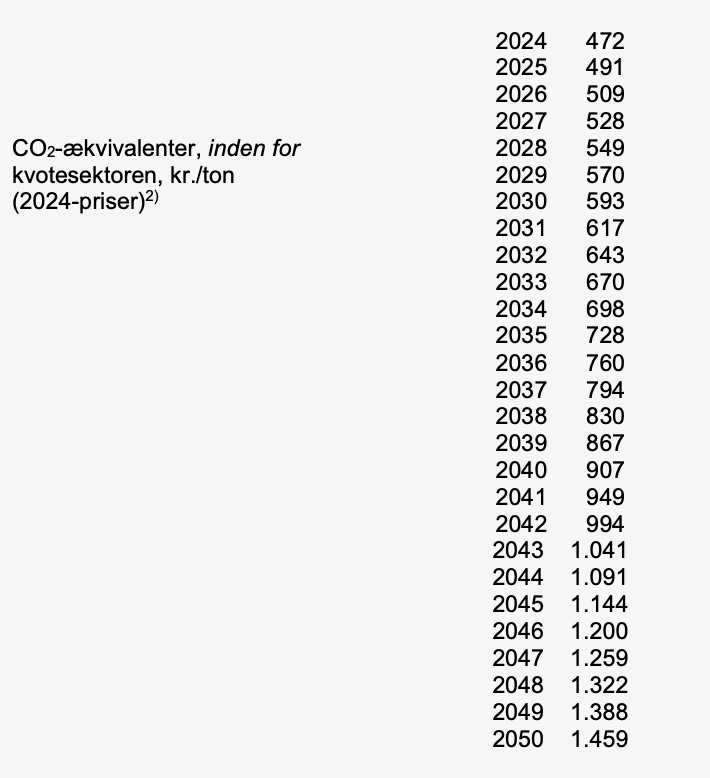
\includegraphics[scale=0.65]{2.png}
     \caption{Oversigt over CO2e priser}
     \label{Figur 2}
\end{figure} 

Det fremgår desuden af vejledningen for samfundsøkonomi konsekvensberegninger, at: \textit{estimater af fordele og ulemper i den
samfundsøkonomiske vurdering er baseret på en række antagelser om prognoser/fremskrivninger, variable og parametre. Der bør foretages
følsomhedsberegninger for at klarlægge, hvilken betydning værdien af en given variabel eller parameter har for udfaldet af den samfundsøkonomiske vurdering}. Et eksempel på sådanne følsomhedsberegning er, at benytte nedenstående CO2e priser fra klimarådet fremfor dem præsenteret i figur 16. 

\begin{figure}[h]
     \centering
     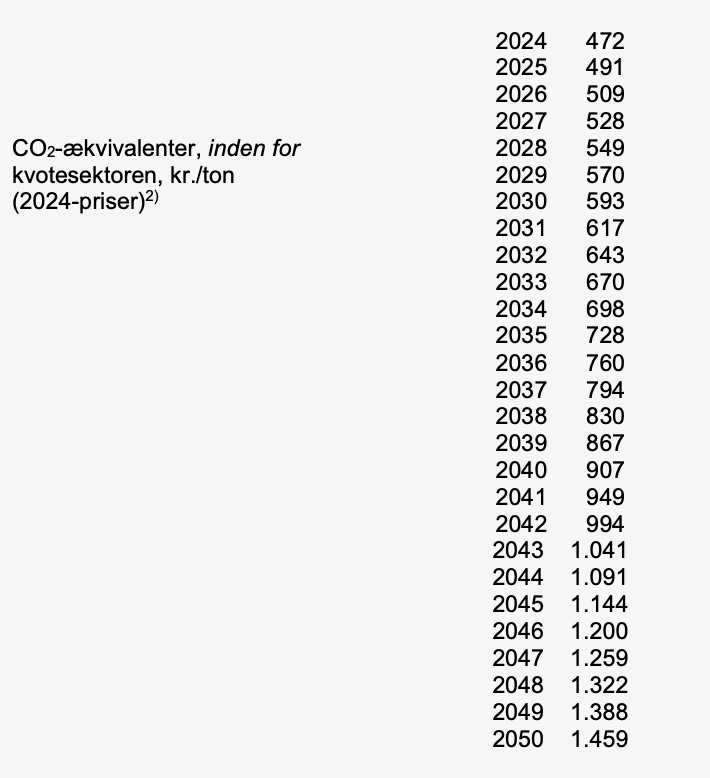
\includegraphics[scale=0.65]{2.png}
     \caption{Oversigt over CO2e priser (klimarådet)}
     \label{Figur 2}
\end{figure} 

Det gælder generelt, at de samfundsøkonomiske konsekvensberegninger viser et \textbf{langt} bedre resultat (højere NPV og højere IRR/MIRR), fordi der tages højde for eksternaliteter, og særligt sparet tid er en stor driver. 

\vspace{10 pt}

Bent Flyvbjerg (dansk professor ved Oxford) har studeret offentlige anlægsinvesteringer og fundet, at man systematisk overvurderer indtægter og undervurderer udgifter. Han kalder fænomenet for megaprojekters jernlov og forklarer det ved: 

\begin{itemize}
    \item ``Optimism bias" and ``Planning fallacy" (adfærdsøkonomi)
    \item Strategisk misrepræsentation
    \item Politikere egeninteresse er kortsigtet – til næste valg.
    \item Politikere vil gerne lægge navn til offentlige mega projekter.
    \item Regionale vs nationale interesser og det representative demokrati (Ex: Jyske Motorveje).
    \item Principal-agent problemer: Politikere kan ikke detailstyre.
    \item Det offentlige har svære ved at styre agenter... og derfor bliver de snydt/overfaktureret (VVS arbejde i NBB).
        \item Survival of the unfittest: Jo mere en projektkalkule misrepræsenterer gevinster og omkostninger, jo større chance har den for at blive vedtaget (alt andet lige)
        \item Når først noget er vedtaget skal det gennemføres (Ex: Niels Bohr Bygningen) – the Ratchet Effect.
\end{itemize}



















\newpage
\section{Appendix}

\begin{figure}[h]
     \centering
     \includegraphics[scale=0.2]{bogføring.jpeg}
     \caption{Bogføring af transaktioner i 'Viking Væv \& Design'}
     \label{Figur 2}
\end{figure} 





\end{document}